\part[Fisica 2]{\texorpdfstring{Fisica 2\\\vspace{1cm}\large{Elettromagnetismo nel vuoto e nella materia, onde elettromagnetiche, ottica}}{Fisica 2}}

\begin{savequote}[6cm]
  Considerate la vostra semenza:\\
  fatti non foste a viver come bruti,\\
  ma per seguir virtute e canoscenza.
  \qauthor{Inferno, canto XXVI}
\end{savequote}



\chapter{Campi}
\minitoc
Il campo \index{campo|(} è uno stato fisico dello spazio o della materia che vi è contenuta. Le cause del campo sono le sorgenti\index{sorgenti!del campo}, per esempio nel caso del campo gravitazionale le masse, in quello elettrostatico le cariche; le sorgenti possono essere descritte in modo puntiforme cioè concentrate o distribuite, quindi è come densità. Le cause del campo e il campo sono legate dalle leggi del campo\index{leggi! del campo}. Il campo è espresso attraverso le funzioni del campo\index{funzione!del campo}.

Le leggi del campo possono essere espresse come:
\begin{description}
  \item[leggi locali] \index{leggi!locali}danno il valore del campo in un punto, come esso varia in funzione delle sorgenti; sono leggi differenziali;
  \item[leggi globali] \index{leggi!globali}danno una valutazione complessiva, su una superficie o un volume; sono leggi integrali.
\end{description}

Il problema generale è risolvere le leggi del campo per passare dalla conoscenza delle cause alla conoscenza del campo.

Il campo può essere:
\begin{description}
  \item[scalare] \index{campo!scalare}cioè una funzione che associa ad ogni punto dello spazio una grandezza scalare, per esempio la temperatura di una stanza. Dal punto di vista matematico sarà una funzione $:\field{R}^3\to\field{R}$;
  \item[vettoriale] \index{campo!vettoriale}cioè una funzione che associa ad ogni punto dello spazio una grandezza vettoriale, per esempio il campo gravitazionale. Dal punto di vista matematico sarà una funzione $:\field{R}^3\to\field{R}^3$.
\end{description}
Dato un campo scalare possiamo definire superficie di livello \index{superficie! di livello}le superfici il luogo dei punti dove il campo assume un certo valore costante.
\index{campo|)}
\section{Richiami di algebra vettoriale}
\[
  (A\times B)_x=A_yB_z-A_zB_y\quad(A\times B)_y=A_zB_x-A_xB_z\quad(A\times B)_z=A_xB_y-A_yB_x
\]
\[A\cdot(A\times B)=0\]
\[A\cdot(B\times C)=C\cdot(A\times B)=B\cdot(C\times A)\]
\[(A\times B)\times C=B(A\cdot C)-A(B\cdot C)\]
\[A\times(B\times C)=B(A\cdot C)-C(A\cdot B)\]
\section{Operatori differenziali}
\subsection{Gradiente\index{gradiente}}
\begin{Def}
  Sia $\varphi=\varphi(x,y,z)$, definiamo il gradiente di $\varphi(x,y,z)$
  \[\grad({\varphi})=\frac{\partial \varphi}{\partial x}\ver \imath+\frac{\partial \varphi}{\partial y}\ver \jmath+\frac{\partial\varphi}{\partial z}\ver k=\ve\nabla\varphi\]
\end{Def}
Da un campo scalare siamo passati ad uno vettoriale. L'operatore $\ve\nabla$ nabla\index{nabla}\index{nabla@$\ve\nabla$|see{nabla}} è $\left(\frac{\partial}{\partial x},\frac{\partial}{\partial y},\frac{\partial}{\partial z}\right)$. Possiamo anche dire, sommando i differenziali lungo le componenti che:
\begin{equation}
  \label{differenziale1}
  \ud \varphi=\frac{\partial\varphi}{\partial x}\ud x+\frac{\partial\varphi}{\partial y}\ud y+\frac{\partial\varphi}{\partial z}\ud z=\ve\nabla\varphi\cdot\ud \ve l\end{equation}
\subsection{Derivata direzionale\index{derivata!direzionale}}
Dall'equazione \eqref{differenziale1} ricaviamo:
\begin{Def}Derivata direzionale di $\varphi$ lungo la direzione di $\ve v$ (versore):
  \begin{equation}
    \frac{\ud\varphi}{\ud \ve v}(\ve x)=\lim_{t\to 0}\frac{\varphi(\ve x+t\ve v)-\varphi(\ve x)}{t}
  \end{equation}
\end{Def}
se $\varphi$ è differenziabile:
\begin{equation}
  \label{differenziale2}
  \frac{\ud \varphi}{\ud \ve v}=\ve\nabla\varphi\cdot{\ve v}
\end{equation}

Il gradiente è sempre perpendicolare alle superfici di livello, infatti se $\ud\ve l$ è parallelo alla superficie di livello allora per definizione $\ud \varphi=0$ e abbiamo:
\[\ve\nabla\varphi\cdot\ud \ve l=\ud\varphi=0\]
La direzione del gradiente è la direzione di massima variazione del campo. Se possiamo esprimere un campo vettoriale come gradiente di un campo scalare allora il campo vettoriale è conservativo\index{campo!conservativo}:
\begin{Teo}
  \label{teo_conservativo1}
  \[\exists \varphi(x,y,z):\quad \ve F(x,y,z)=\ve\nabla\varphi(x,y,z)\Rightarrow\text{$\ve F$ è conservativo}\]
\end{Teo}
dal punto di vista matematico vuol dire che la forma differenziale $\ve F\cdot\ud\ve r$ ha un potenziale e quindi è esatta.
\subsection{Integrale di linea\index{integrale!di linea}}
\begin{Def}
  Sia $\ve F(x,y,z)$ la funzione di un campo vettoriale, siano $P_1$ e $P_2$ due punti di una curva $\Gamma$. Dividiamo $\Gamma$ in tanti $\Delta \ve l_i$ tra $P_1$ e $P_2$. Sia $\ve F_i$ il valore del campo nel punto di applicazione di $\Delta \ve l_i$, allora l'integrale di linea della funzione $\ve F(x,y,z)$ lungo la curva $\Gamma$ tra $P_1$ e $P_2$:
  \begin{equation}
    \label{integrale_linea}
    \int_\Gamma \ve F(x,y,z)\cdot \ud\ve l=\lim_{\Delta l_i\to 0}\sum\ve F_i\cdot\Delta\ve l_i
  \end{equation}
\end{Def}
Supponiamo che $\ve F$ sia conservativo, allora (per il teorema \ref{teo_conservativo1}) possiamo riscrivere l'integrale di linea \eqref{integrale_linea} come:
\begin{equation}
  \label{conservativo00}
  \int_\Gamma \ve F(x,y,z)\cdot \ud \ve l=\int_\Gamma \ve\nabla\varphi(x,y,z)\cdot\ud\ve l=\int_\Gamma \ud\varphi=\varphi(P_2)-\varphi(P_1)
\end{equation}
cioè non è in funzione della curva. Abbiamo allora una definizione di campo conservativo data dalla \eqref{conservativo00}\index{campo!conservativo}\footnote{l'ipotesi che manca è che l'insieme su cui è definito il campo sia un aperto stellato}. Consideriamo $\Gamma$ una linea chiusa, allora sempre nel caso conservativo si ha:
\begin{equation}
  \label{circ00}
  \oint_\Gamma\ve F(x,y,z)\cdot\ud\ve l=\underset{P_2}{\overset{P_1}{\int_{\Gamma_1}}}\ve F\cdot\ud\ve l+\underset{P_1}{\overset{P_2}{\int_{\Gamma_2}}}\ve F\cdot\ud\ve l=0
\end{equation}
per ogni $\Gamma$, che è equivalente alla \eqref{conservativo00}. La quantità nella \eqref{circ00} è chiamata circuitazione di $\ve F$\index{circuitazione}.
\subsubsection{Campo conservativo}
Abbiamo ora due modi per esprimere il concetto che $\ve F(x,y,z)$ è conservativo, uno dato dal teorema \ref{teo_conservativo1} e l'altro dalla \eqref{circ00}\index{campo!conservativo}:
\begin{description}
  \item[forma differenziale (locale)]\[\ve F(x,y,z)=\grad\varphi(x,y,z)\]
  \item[forma integrale (globale)]\[\oint\ve F(x,y,z)\cdot\ud\ve l=0\]
\end{description}
\subsection{Flusso\index{flusso}}
\begin{Def}
  Il flusso uscente attraverso la superficie $S$ del campo $\ve F$ è definito come:
  \[\phi_S(\ve F)=\int_S \ve F\cdot \ve n\, \ud a\]
\end{Def}
operativamente significa:
\[\lim_{\Delta A_k\to 0}\sum \ve F_n\cdot \ve n_k\,\Delta A_k\]
dove $\Delta A_k$ sono le areole in cui abbiamo scomposto la superficie $S$, $\ve n_k$ le loro normali e $\ve F_n$ il valore del campo al centro delle areole. Per una superficie chiusa si parla di:
\[\phi_S(\ve F)=\oint_S \ve F\cdot \ve n\, \ud a\]
\subsubsection{normale\index{vettore!normale}\index{normale}}
La normale è un vettore di modulo unitario, ortogonale alla superficie, per una superficie chiusa è orientato verso l'esterno (e infatti si parla di flusso uscente), mentre per una superficie generica dipende dall'orientamento del contorno. A volte al posto di usare il concetto di normale si preferisce usare il concetto di area orientata, che diventa un vettore ($\ud \ve a=\ve n\,\ud a$):
\[\phi_S(\ve F)=\oint_S \ve F\cdot \ud \ve a\]
\subsubsection{flusso netto\index{flusso!netto}}
Se dividiamo una superficie $S$ con un taglio la dividiamo in due superfici: $S_a$ e $S_b$; sia $S_{ab}$ la superficie di taglio. Sia $S_1=S_a\cup S_{ab}$ e $S_2=S_b\cup S_{ab}$. I flussi che escono dalla superfici saranno:
\[\phi_{S_1}(\ve F)=\int_{S_a}\ve F\cdot\ve n\,\ud a+\int_{S_{ab}}\ve F\cdot\ve n_1\,\ud a\]
\[\phi_{S_2}(\ve F)=\int_{S_b}\ve F\cdot\ve n\,\ud a+\int_{S_{ab}}\ve F\cdot\ve n_2\,\ud a\]
ma essendo la normale orientata verso l'esterno del volume:
\[\ve n_1=-\ve n_2\]
Quindi il flusso è la somma dei flussi delle superfici aperte $S_a$ e $S_b$:
\[\oint_S\ve F\cdot\ve n\,\ud a=\int_{S_a}\ve F\cdot\ve n\,\ud a+\int_{S_b}\ve F\cdot \ve n\,\ud a\]
Possiamo ripetere il procedimento e suddividere ulteriormente a piacimento.

Se il flusso uscente è maggiore di zero vuol dire che all'interno ci sono sorgenti positive, se minore di zero sorgenti negative. Si intende sempre somma delle sorgenti.
\subsection{Divergenza\index{divergenza}}
La divergenza non è altro che il flusso in un punto, cioè su una superficie infinitesima.
\begin{Def}
  \[\diver \ve F(x,y,z)=\lim_{V\to 0}\oint_S \frac{\ve F\cdot \ve n\,\ud a}{V}\]
  con $S$ la superficie che racchiude $V$.
\end{Def}

Possiamo dire che se la divergenza nel punto è nulla allora in quel punto non c'è accumulo, se positiva c'è una densità positiva di sorgenti, se negativa una densità negativa.

Prendiamo per esempio un parallelepipedo, allineato con gli assi cartesiani e con uno spigolo in coordinate $(x,y,z)$. Siano le sue dimensioni $\Delta x$, $\Delta y$, $\Delta z$. Conoscendo il flusso sulla faccia $1$ nella direzione $x$ con Taylor al primo ordine possiamo calcolare il flusso sulla faccia $2$:
\[\ve F(2)= F_x(1)+\frac{\partial F_x}{\partial x}\Delta x\]
Risulta allora:
\[\phi(1)=- F_x(1)\Delta y\Delta z\]
\[\phi(2)=\left[F_x(1)+\frac{\partial F_x}{\partial x}\Delta x\right]\Delta y\Delta z\]
\[\phi(1\cup 2)=\frac{\partial F_x}{\partial x}\Delta x\Delta y\Delta z\]
e similmente per le altre facce, il flusso totale è allora:
\[\int_{\text{cubo}} \ve F\cdot\ud a=\left(\frac{\partial F_x}{\partial x}+\frac{\partial F_y}{\partial y}+\frac{\partial F_z}{\partial z}\right)\Delta x\Delta y\Delta z\]


Se ora facciamo $\Delta V\to 0$ che risolve tutti i problemi degli ordini trascurati nello sviluppo di Taylor abbiamo che:
\begin{equation}\label{div01}
  \diver \ve F(x,y,z)=\left(\frac{\partial F_x}{\partial x}+\frac{\partial F_y}{\partial y}+\frac{\partial F_z}{\partial z}\right)=\ve\nabla\cdot\ve F\end{equation}

\subsection{Teorema della divergenza\index{divergenza!teorema}\index{teorema!della divergenza}}
Dall'equazione \eqref{div01} possiamo scrivere sostituendo la definizione di divergenza:
\[\frac{\ud}{\ud V}\int_S \ve F\cdot\ve n\,\ud a=\ve\nabla\cdot\ve F\]
allora:
\begin{Teo}[divergenza]
  Sia $S$ la superficie che delimita il volume $V$:
  \[\int_V\diver \ve F\,\ud v=\int_S\ve F\cdot\ve n\,\ud a\]
\end{Teo}
Conoscendo la divergenza possiamo calcolare il flusso attraverso $S$. Possiamo riferirci anche a solo una direzione:
\[\int_V\frac{\partial F_x(x,y,z)}{\partial x}\ud v=\int_S F_x(x,y,z)\cos(n,x)\,\ud a\]
\subsubsection{Campo solenoidale\index{campo!solenoidale}}
Un campo $\ve F$ si dice solenoidale se:
\begin{description}
  \item[legge differenziale]\[\forall x,y,z\qquad \diver\ve F(x,y,z)=0\]
  \item[legge integrale]\[\forall S \qquad\phi_S(\ve F)=0\]
\end{description}
\section{Circuitazione\index{circuitazione}}
L'integrale di un campo vettoriale $\ve C(x,y,z)$ calcolato su una linea chiusa $\Gamma$ è chiamato circuitazione. Se dividiamo il percorso in pezzetti $\ud \ve s$ tangenti, allora la componente del campo parallela a $\ud \ve s$ sarà $\ud \ve s\cdot \ve C$ e la circuitazione è
\begin{equation}
  \oint_\Gamma \ve C\cdot\ud\ve s
\end{equation}
Se dividiamo  $\Gamma$ in due cicli $\Gamma_1$ e $\Gamma_2$ appare chiaro che:
\[\oint_{\Gamma_1} \ve C\cdot\ud \ve s+\oint_{\Gamma_2} \ve C\cdot\ud\ve s=\oint_\Gamma\ve C\cdot\ud\ve s\]
Possiamo continuare così fino ad ottenere dei cicli chiusi piccoli a piacere, il risultato sarebbe lo stesso in quanto le linee adiacenti si annullerebbero e rimarrebbe solo la parte esterna.
\subsection{Teorema di Stokes\index{teorema!di Stokes}}
Immaginiamo un rettangolo orientato come gli assi di lati $\ud x$ e $\ud y$. Sia $A$ il vertice sinistro inferiore di coordinate $(x,y)$ (vedi figura \ref{stokes_ret}). Vogliamo calcolare la circuitazione del campo $\ve C(\ve r)$ sul rettangolo. Sviluppando con Taylor al primo ordine:
\[C_x(C)=C_x(A)+\frac{\partial C_x}{\partial y}\ud y\]
\[\left[C_x(A)-C_x(C)\right]\ud x=-\frac{\partial C_x}{\partial y}\ud x\ud y\]
\[\left[C_y(B)-C_y(D)\right]\ud x=\frac{\partial C_y}{\partial y}\ud x\ud y\]
\begin{figure}[htbp]
  \centering
  \begin{tikzpicture}[scale=0.8]
\draw (1,1) node[below left]{$A$} -- (1,5) node[above left]{$D$} -- (7,5)
node[above right]{$C$} -- (7,1) node[below right]{$B$} -- cycle;

\draw[<-] (4,5) -- (7,5);
\draw (4,1) node[below] {$\ud x$};
\draw (7,3) node[right] {$\ud y$};

\draw[->] (0,0) -- (9,0) node[right] {$x$};
\draw[->] (0,0) -- (0,6) node[right] {$y$};

\end{tikzpicture}

  \label{stokes_ret}
  \caption{teorema di Stokes.}
\end{figure}
La circuitazione è
\begin{align*}
  \oint \ve C\cdot\ud\ve s & =C_x(A)\ud x+C_y(B)\ud y-C_x(C)\ud x-C_y(D)\ud y
  \\
                           & =\left(\frac{\partial C_y}{\partial x}-\frac{\partial C_x}{\partial y}\right)\ud x\ud y=\left(\ve \nabla\times\ve C\right)_z\ud a
\end{align*}
$z$ in questo caso è la componente normale alla superficie. In generale:
\begin{Teo}[Stokes]
  \begin{equation}
    \oint_\Gamma\ve C\cdot\ud\ve s=\int_S\left(\ve\nabla\times\ve C\right)\cdot\ve n\,\ud a
  \end{equation}
\end{Teo}

\section{Coordinate\index{coordinate|(}\index{sistema!di riferimento}}
Consideriamo un sistema di coordinate in $\field{R}^n$, fissiamo una base $\{\ver e_j\}_{j=1}^n$, ogni vettore lo possiamo scrivere univocamente nella forma:
\[\ve r=u_1\ver e_1+\cdots+u_n\ver e_n\]
\subsection{Coordinate curvilinee}
\begin{Def}[Superficie Coordinata]
  Una superficie coordinata \index{superficie!coordinata} è il luogo dei punti dove:
  \[u_j=\const\]
  con $j$ fissato.
\end{Def}
\begin{Def}[Linea Coordinata]
  Una linea coordinata \index{linea!coordinata} è il luogo dei punti dove:
  \[
    \left\{\begin{array}{l}
      u_j=\const \\
      u_k=\const
    \end{array}\right.
  \]
  con $j\neq k$ fissati.
\end{Def}
\begin{Def}[Versori delle coordinate\index{versore}]
  Il versore delle coordinate $\ver e_j$ è il vettore ortogonale alle superfici coordinate $u_j=\const$ e tangente alle linee coordinate $u_{\forall k\neq j}=\const$.
\end{Def}
Consideriamo ora solo $\field{R}^3$. Un cambiamento di coordinate è una trasformazione biunivoca, non necessariamente lineare, del tipo:
\[
  \left\{\begin{array}{l}
    u_1=u_1(x,y,z) \\
    u_2=u_2(x,y,z) \\
    u_3=u_3(x,y,z) \\
  \end{array}\right.
\]
\subsubsection{Versori}
Conoscendo la trasformazione delle coordinate possiamo trovare nuovi versori sfruttando il fatto che la distanza deve rimanere invariante. Consideriamo la distanza infinitesima:
\begin{equation}
  \ud s = \ud x\ver i + \ud y\ver j + \ud z\ver k
\end{equation}
nelle coordinate generiche $u_i$ questo si scrive come:
\begin{equation}
  \ud s = \ud u_1\ve e_1 + \ud u_2\ve e_2 + \ud u_3\ve e_3
\end{equation}
differenziando la prima, considerando $x,y,z$ come funzione delle nuove coordinate si trova:
\begin{equation}
  \begin{aligned}
    \ud u_1\ve e_1 + \ud u_2\ve e_2 + \ud u_3\ve e_3 = & \left(\frac{\partial x}{\partial u_1}\ud u_1 + \frac{\partial x}{\partial u_2}\ud u_2 +  \frac{\partial x}{\partial u_3}\ud u_3\right)\ver i \\
    +                                                  & \left(\frac{\partial y}{\partial u_1}\ud u_1 + \frac{\partial y}{\partial u_2}\ud u_2 +  \frac{\partial y}{\partial u_3}\ud u_3\right)\ver j \\
    +                                                  & \left(\frac{\partial z}{\partial u_1}\ud u_1 + \frac{\partial z}{\partial u_2}\ud u_2 +  \frac{\partial z}{\partial u_3}\ud u_3\right)\ver k
  \end{aligned}
\end{equation}
uguagliando i termini che moltiplicano $\ud u_i$, il versore $i$--esimo delle nuove coordinate si scrive:
\[\ve e_i=\left(\dfrac{\partial x}{\partial u_i}\ver \imath+\dfrac{\partial y}{\partial u_i}\ver \jmath+\dfrac{\partial z}{\partial u_i}\ver k\right)\]
Gli $\ve e_i$ non sono normalizzati, introduciamo i fattori di normalizzazione:
\[D_i=\sqrt{\left(\frac{\partial x}{\partial u_i}\right)^2+\left(\frac{\partial y}{\partial u_i}\right)^2+\left(\frac{\partial z}{\partial u_i}\right)^2}\]
detti \index{fattore!di scala} fattori di scala. Quindi i versori $\ver e_i$:
\begin{equation}
  \ver e_i = \frac{\ve e_i}{D_i} = \dfrac{\left(\dfrac{\partial x}{\partial u_i}\ver \imath+\dfrac{\partial y}{\partial u_i}\ver \jmath+\dfrac{\partial z}{\partial u_i}\ver k\right)}{D_i}
\end{equation}
\subsubsection{Spostamento infinetisimo}
\begin{equation}
  \ud s = \ud u_1 D_1 \ver e_1 + \ud D_2 u_2\ver e_2 + \ud u_3 D_3 \ver e_3
\end{equation}
\subsubsection{Volume elementare}
\begin{equation}
  \ud V = D_1D_2D_3 \ud u_1\ud u_2\ud u_3
\end{equation}
\subsubsection{Gradiente}
\begin{equation}
  \ve\nabla\phi = \frac{1}{D_1}\frac{\partial\phi}{\partial u_1} + \frac{1}{D_2}\frac{\partial\phi}{\partial u_2} + \frac{1}{D_3}\frac{\partial\phi}{\partial u_3}
\end{equation}
\subsubsection{Divergenza}
\begin{equation}
  \ve\nabla\cdot\ve A = \frac{1}{D_1D_2D_3}\left[\frac{\partial}{\partial u_1}(D_2D_3 A_1) + \frac{\partial}{\partial u_2}(D_3D_1 A_2) + \frac{\partial}{\partial u_3}(D_1D_2 A_3)\right]
\end{equation}
\subsubsection{Rotore}
\begin{equation}
  \ve\nabla\times\ve A = \frac{1}{D_1D_2D_3}\det\begin{pmatrix}
    D_1\ver e_1                    & D_2\ver e_2                    & D_3\ver e_3                    \\
    \dfrac{\partial}{\partial u_1} & \dfrac{\partial}{\partial u_2} & \dfrac{\partial}{\partial u_3} \\
    D_1\ve A_1                     & D_2\ve A_2                     & D_3\ve A_3\end{pmatrix}
\end{equation}
\subsubsection{Laplaciano}
\begin{equation}
  \nabla^2 \phi = \frac{1}{D_1D_2D_3}\left[
    \frac{\partial}{\partial u_1}\left(\frac{D_2D_3}{D_1}\frac{\partial\phi}{\partial u_1}\right)
    + \frac{\partial}{\partial u_2}\left(\frac{D_3D_1}{D_2}\frac{\partial\phi}{\partial u_2}\right)
    + \frac{\partial}{\partial u_3}\left(\frac{D_1D_2}{D_3}\frac{\partial\phi}{\partial u_3}\right)
    \right]
\end{equation}

\subsection{Coordinate cartesiane\index{coordinate!cartesiane}}
\subsubsection{Superfici coordinate}
Per definizione una superficie coordinata è
\[
  \left\{\begin{array}{l}
    x=\const \\
    y=t      \\
    z=t\end{array}\right.
  \quad
  \text{o}
  \quad
  \left\{\begin{array}{l}
    x=t      \\
    y=\const \\
    z=t\end{array}\right.
  \quad
  \text{o}
  \quad
  \left\{\begin{array}{l}
    x=t \\
    y=t \\
    z=\const\end{array}\right.
\]
che sono tre famiglie di piani, ognuna con piani ortogonali ad un asse diverso.
\subsubsection{Linee Coordinate}
\[
  \left\{\begin{array}{l}
    x=\const \\
    y=\const \\
    z=t\end{array}\right.
  \quad
  \text{o}
  \quad
  \left\{\begin{array}{l}
    x=t      \\
    y=\const \\
    z=\const\end{array}\right.
  \quad
  \text{o}
  \quad
  \left\{\begin{array}{l}
    x=\const \\
    y=t      \\
    z=\const\end{array}\right.
\]
che sono tre famiglie di rette, ognuna con rette parallele ad un asse diverso\footnote{$\const$ indica costanti non necessariamente uguali, quindi nella prima famiglia non è detto che $x=y$}.
\subsection{Coordinate cilindriche\index{coordinate!cilindriche}}
La trasformazione rispetto alle coordinate cartesiane è
\[\left\{\begin{array}{l}
    x=\rho\cos\theta \\
    y=\rho\sin\theta \\
    z=w              \\
  \end{array}\right.
\]

\subsubsection{Superfici coordinate}
Se fissiamo $\rho=\const$ e facciamo variare le altre due coordinate otteniamo un cilindro; se fissiamo $\theta$ un semipiano perpendicolare al piano individuato dagli assi cartesiani $xy$, che ha origine sulla retta $x=y=0$; se fissiamo $w$ otteniamo un piano come in coordinate cartesiane.

\subsubsection{Linee coordinate}
Se facciamo variare solo $\rho$ otteniamo una semiretta uscente dall'origine; se facciamo variare solo $\theta$ una circonferenza che giace in un piano parallelo al piano $xy$; se facciamo variare solo $w$ otteniamo una retta parallela all'asse $z$.

\subsubsection{Versori}
\[D_\rho=\sqrt{\left(\frac{\partial x}{\partial\rho}\right)^2+\left(\frac{\partial y}{\partial \rho}\right)^2+\left(\frac{\partial z}{\partial \rho}\right)^2}=\sqrt{\cos^2\theta+\sin^2\theta}=1\]
\[D_\theta=\sqrt{\left(\frac{\partial x}{\partial\theta}\right)^2+\left(\frac{\partial y}{\partial \theta}\right)^2+\left(\frac{\partial z}{\partial \theta}\right)^2}=\sqrt{\left(-\rho\sin\theta\right)^2+\left(\rho\cos\theta\right)^2}=\rho\]
\[D_w=1\]
\[\ver e_\rho=\frac{\frac{\partial x}{\partial\rho}\ve i+\frac{\partial y}{\partial\rho}\ve j+\frac{\partial z}{\partial\rho}\ve k}{D_\rho}=\cos\theta\ve i+\sin\theta\ve j\]
\[\ver e_\theta=\frac{\frac{\partial x}{\partial\theta}\ve i+\frac{\partial y}{\partial\theta}\ve j+\frac{\partial z}{\partial\theta}\ve k}{D_\theta}=-\sin\theta\ve i+\cos\theta\ve j\]
\[\ver e_w=\ve k\]
Notare che $\ver e_\theta$ e $\ver e_\rho$ sono ortogonali e che ogni vettore si scrive come $\ve r=r\ver e_\rho$.

\subsection{Coordinate sferiche\index{coordinate!sferiche}}
La trasformazione dalla coordinate cartesiane e quella inversa sono:
\[\left\{\begin{array}{l}
    x=\rho\sin\theta\cos\varphi \\
    y=\rho\sin\theta\sin\varphi \\
    z=\rho\cos\theta            \\
  \end{array}\right.
  \qquad
  \left\{\begin{array}{l}
    \rho=\sqrt{x^2+y^2+z^2}                \\
    \theta=\arctan\frac{\sqrt{x^2+y^2}}{z} \\
    \varphi=\arctan\frac{y}{x}             \\
  \end{array}\right.
\]
con $\rho\in(0,+\infty)$, $\theta\in[0,\pi]$, $\varphi\in[0,2\pi)$.

\subsubsection{Superfici Coordinate}
Fissando solo $\rho$ si ottiene una sfera; fissando solo $\theta$ un cono; fissando solo $\varphi$ si ottiene un semipiano.
\subsubsection{Linee Coordinate}
Variando solo $\rho$ si ottiene una semiretta; variando solo $\theta$ una circonferenza; variando solo $\varphi$ una circonferenza.
\subsubsection{Versori}
\[D_\rho=1\qquad D_\theta=\rho\qquad D_\varphi=\varphi\sin\theta\]
\[\ver e_\rho=\sin\theta\cos\varphi\ver \imath+\sin\theta\cos\varphi\ver \jmath+\cos\theta\ver k\]
\[\ver e_\theta=\cos\theta\cos\varphi\ver \imath+\cos\theta\sin\varphi\ver \jmath-\sin\theta\ver k\]
\[\ver e_\varphi=-\sin\varphi\ver \imath+\cos\varphi\ver \jmath\]
\index{coordinate|)}

\chapter{Elettrostatica\index{elettrostatica}}
\minitoc
Tutta l'elettrodinamica nel vuoto può essere descritta con le quattro equazioni di Maxwell\index{Maxwell}
\index{equazioni!di Maxwell} scritte nel sistema MKS:
\begin{subequations}
  \begin{gather}
    \ve\nabla\cdot\ve E=\frac{\rho}{\varepsilon_0}\\
    \ve\nabla\times\ve E=-\frac{\partial \ve B}{\partial t}\\
    \ve\nabla \cdot \ve B=0\\
    c^2\ve\nabla\times \ve B=\frac{\partial \ve E}{\partial t}+\frac{\ve J}{\varepsilon_0}
  \end{gather}
\end{subequations}
oppure nel sistema CGS:
\begin{subequations}
  \begin{gather}
    \ve\nabla\cdot\ve E=4\pi\rho\\
    \ve\nabla\times\ve E=-\frac{1}{c}\frac{\partial \ve B}{\partial t}\\
    \ve\nabla \cdot \ve B=0\\
    \ve\nabla\times \ve B=\frac{1}{c}\frac{\partial \ve E}{\partial t}+\frac{4\pi}{c}\ve J
  \end{gather}
\end{subequations}

In elettrostatica si studia il campo elettrico $\ve E$ in condizioni stazionarie, che non dipendono dal tempo, quindi le equazioni di Maxwell nel vuoto diventano:
\begin{subequations}
  \begin{gather}
    \ve\nabla\cdot\ve E=\frac{\rho}{\varepsilon_0}\\
    \ve\nabla\times\ve E=0
  \end{gather}
\end{subequations}
si parla allora di campo elettrostatico.
\section{Carica\index{carica elettrica}}
La carica è una proprietà della materia, tanto quanto la massa. La carica può essere positiva o negativa. La più piccola è quella dell'elettrone, $-e\simeq\SI{-1.6E-19}{\coulomb}$, tutte le altre sono multipli interi di essa.
\section{Forza di Coulomb\index{forza!di Coulomb}}
Partiamo da una legge sperimentale che riguarda la forza che una carica $q_1$ ferma esercita su una carica $q_2$ ferma nel vuoto:
\begin{equation}
  \label{coulomb01}
  \ve{F}_{12}=K_e\frac{q_1q_2}{r_{12}^2}\ver{r_{12}}
\end{equation}
dove $\ve r_{12}$ è il vettore che individua $q_2$ rispetto a $q_1$ e $\ver r_{12}$ è il vettore unitario orientato come $\ve r_{12}$:
\begin{equation}
  \label{norm02}
  \ver r_{12}=\frac{\ve r_{12}}{\norm{\ve r_{12}}}
\end{equation}

\begin{figure}[htbp]
  \centering
  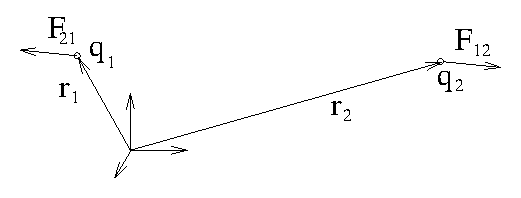
\includegraphics[scale=1]{immagini/fisica2/forza_coulomb}
\end{figure}
La \eqref{coulomb01} la possiamo riscrivere usando la \eqref{norm02}:
\[\ve{F}_{12}=K_e\frac{q_1q_2}{r_{12}^3}\ve{r_{12}}\]
oppure se $\ve r_1$ individua $q_1$ rispetto all'origine e $\ve r_2$ $q_2$:
\[
  \ve{F}_{12}=K_e\frac{q_1q_2}{\norm{\ve r_2-\ve r_1}^3}\left(\ve r_2-\ve r_1\right)
\]
Naturalmente per la terza legge della dinamica:
\[
  \ve F_{12}=-\ve F_{21}
\]
\subsection{Unità di misura}
Un'idea è quella di porre $K_e=1$ e di definire la carica unitaria quella carica che posta alla distanza unitaria da una carica unitaria produce una forza unitaria. Questo è quello che si fa nel sistema CGS Elettrostatico\index{CGS elettrostatico}. Non si definisce a priori la carica, che prende il nome di u.e.s.\@ unità elettrostatica semplice\index{unità elettrostatica semplice}, chiamata anche stat--coulomb\index{stat--coulomb}.

Il secondo modo è di definire a priori la carica, ed è quello che si fa nel Sistema Internazionale. Si definisce coulomb\index{coulomb} quella carica che attraversando un voltametro al nitrato d'argento ($\mathrm{AgNO_3}$) deposita sul catodo una quantità di Ag di \SI{0.00111800}{\gram}. \`E una definizione provvisoria. Si ricava quindi $K_e\simeq \SI{8.8974E9}{\newton\meter\squared\per\coulomb\squared}$. Nell'ambito del SI si è comodo usare il sistema razionalizzato Giorgi\index{Giorgi}\index{sistema!razionalizzato Giorgi}, nella quale $K_e=\frac{1}{4\pi\varepsilon_0}$, $\varepsilon_0\simeq \SI{8.8E-12}{\coulomb\squared\per\newton\metre\squared}$.

Il coulomb e lo stat-coulomb nonostante siano unità della stessa grandezza hanno dimensioni diverse.
\begin{Es}[pendolo magnetico]
  \begin{figure}[htbp]
    \centering
    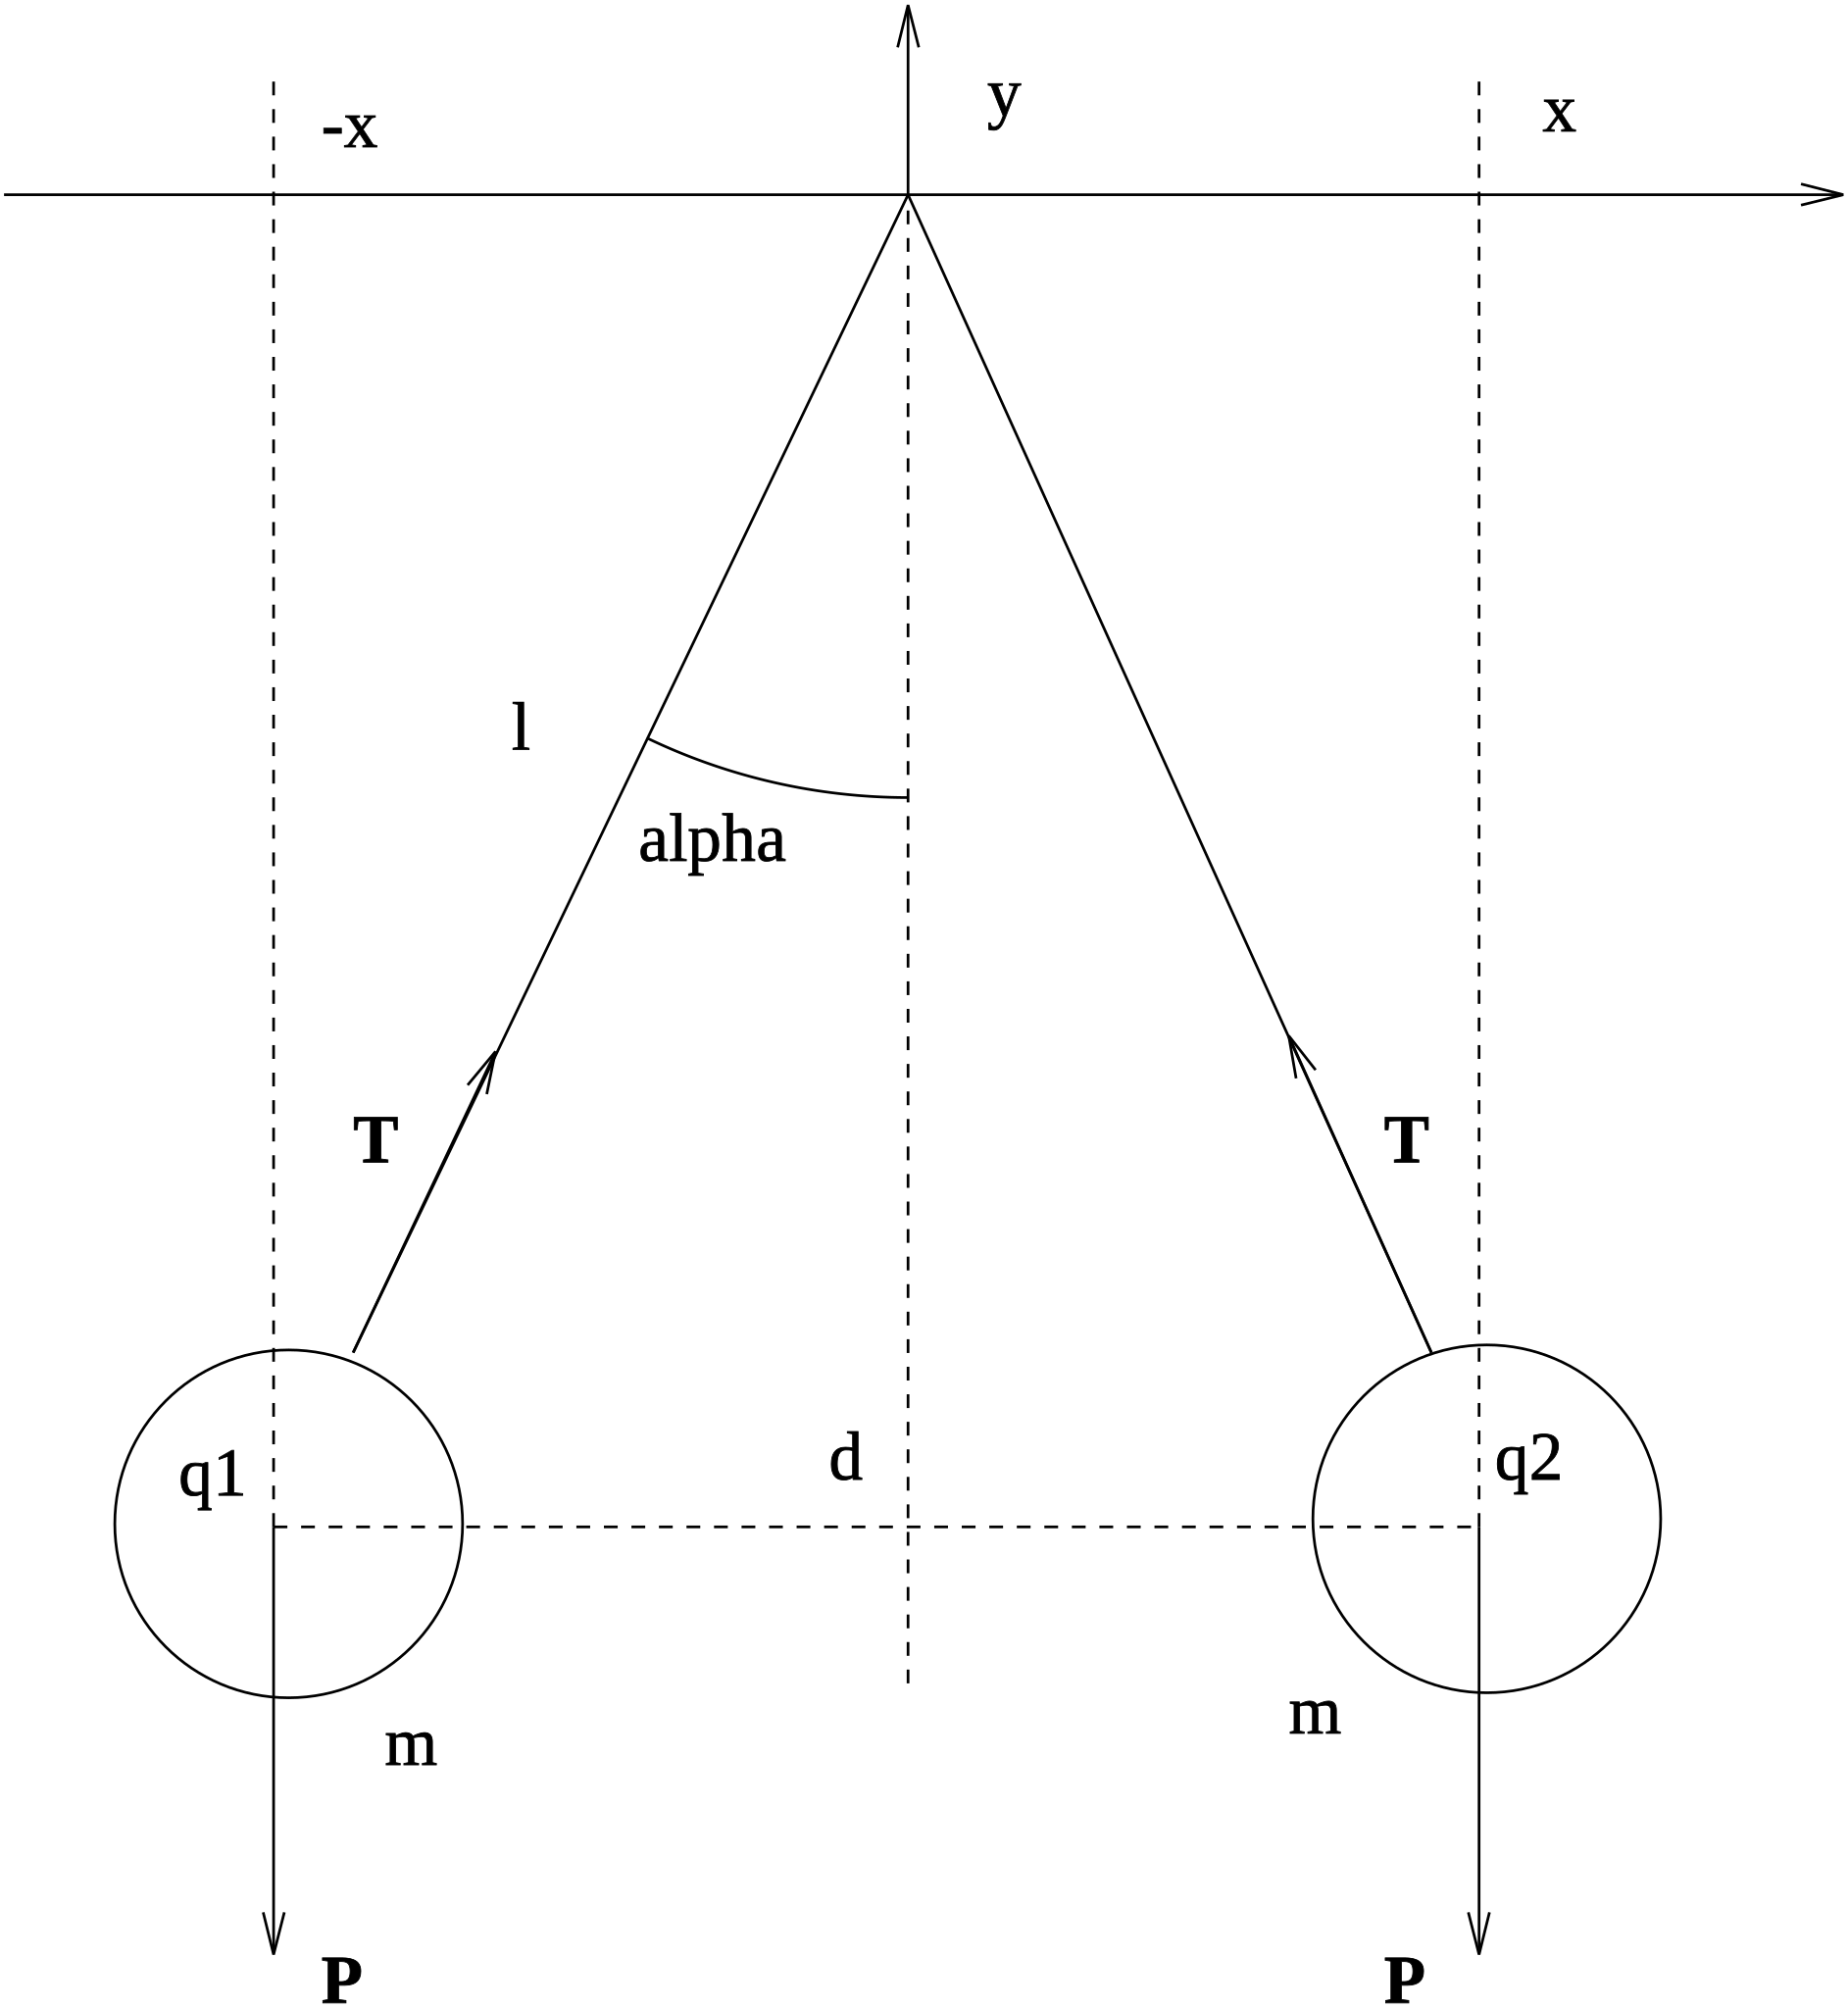
\includegraphics[scale=0.5]{immagini/fisica2/pendolo_carico}
  \end{figure}
\end{Es}
Ci si chiede l'equilibrio del pendolo in figura. Se $q_1q_2<0$ allora l'equilibrio è $x=0$.
\[\ve F_e=\frac{q_1q_2}{4\pi\varepsilon_0}\frac{1}{d^2}\ver e_{q_1,q_2}=\frac{q_1q_2}{4\pi\varepsilon_0}\frac{1}{4x^2}\ver x\]
\[\ve P=-mg\ver \jmath\]
Scomponendo sugli assi e imponendo l'equilibrio:
\[\left\{\begin{array}{l}
    T\sin\alpha\ver \imath-\dfrac{q_1q_2}{4\pi\varepsilon_0}\dfrac{1}{4x^2}\ver \imath=0 \\
    T\cos\alpha\ver \jmath-mg\ver \jmath=0
  \end{array}\right.\]
Dividendo e usando $x=l\sin\alpha$
\[\tan\alpha=\frac{q_1q_2}{16\pi\varepsilon_0mgl^2}\frac{1}{\sin^2\alpha}\]
\[\sin^2\alpha=1-\frac{1}{1+\tan^2\alpha}\qquad\frac{1}{\sin^2\alpha}=\frac{1+\tan^2\alpha}{\tan^2\alpha}\]
\[\tan^3\alpha=\frac{q_1q_2}{16\pi\varepsilon_0mgl^2}(1+\tan^2\alpha)\]
Ipotizziamo che $\alpha\ll 1$, allora $\tan\alpha\simeq\alpha$:
\[\alpha=\sqrt[3]{\frac{q_1q_2}{16\pi\varepsilon_0mgl^2}}\]
Naturalmente se $y_1\neq y_2$ allora le soluzioni potrebbero essere altre. Se scostiamo di poco una massa dalla posizione di equilibrio $x_0=l\alpha$ di $\delta_x=(x-x_0)$ la forza (primo sviluppo di Taylor) risulta:
\[F(x)=F(x_0-\delta_x)=F(x_0)+F'(x_0)\delta_x=F'(x_0)\delta_x\]
l'equazione del moto diventa:
\[m\ddot x=F'(x_0)\delta_x\]


\section{Densità di carica\index{densità di carica}}
Al posto di immaginare la materia come un discreto con cariche puntiformi possiamo immaginarla, a livello macroscopico, come un continuo, definendo una densità di carica volumetrica. Sia $V$ un volume, e $\Delta V$ una porzione di essa. All'interno di $\Delta V$ è contenuta la carica $\Delta q$.
\begin{Def}[Densità carica\index{densità di carica!volumetrica}]
  \[\rho\left({\ve r}\right)=\lim_{\Delta V\to 0}\frac{\Delta q}{\Delta V}=\frac{\ud q}{\ud V}\]
\end{Def}
La carica totale è allora:
\[Q=\int_V\rho(\ve r)\,\ud V\]
Allo stesso modo possiamo definire una densità superficiale di carica \index{densità di carica!superficiale}$\sigma(\ve r)$, o lineare \index{densità di carica!lineare}$\lambda(\ve r)$.
\subsection{Forza}
Usado la densità di carica possiamo riscivere la forma di Coulumb. La forza dell'elementino $\ud V'$ (posto nelle cordinate $\ve r'$) sulla carica puntiforme esterna $q$ è
\[\ud\ve F=\frac{1}{4\pi\varepsilon_0}\frac{q\,\ud q'}{\norm{\ve r-{\ve r}\,^\prime}^3}\left(\ve r-{\ve r}\,^\prime\right)\]
Quindi la forza totale del volume $V$ sulla carica esterna $q$:
\[\ve F=\int_V \ud \ve F=\frac{q}{4\pi\varepsilon_0}\int_V\frac{\
  \rho(\ve r\,^\prime)\left(\ve r-{\ve r}\,^\prime\right)}{\norm{\ve r-{\ve r}\,^\prime}^3}\,\ud V'\]
\section{Campo elettrico\index{campo!elettrico}\index{campo!elettrostatico}}
Fino ad ora abbiamo usato il concetto di azione a distanza\index{azione a distanza},
%\[{\oint\limits_0^1}_{\Gamma}\]
%\[\mathop{{\int\!\!\!\!\!\int}\mkern-21mu \bigcirc}\limits_{3}{{\mathop{\rm{x}}}}\]
%\[\mathop{{\int\!\!\!\!\!\int\!\!\!\!\!\int}\mkern-31.2mu\bigodot}\limits_{0}{{\mathop{\rm x}}}}\]
cioè una carica produce direttamente (o attraverso le linee di forza) una forza su un'altra carica. L'altro modo di pensare è che una carica modifica il campo elettrostatico, il quale produce una forza su un'altra carica. Definiamo il campo elettrostatico:
\[\ve E=\frac{\ve F}{q}\]
con $\ve F$ la forza esercitata dalla carica generante il campo sulla carica esplorativa e $q$ il valore della carica esplorativa, cioè la carica su cui agisce il campo. Può essere interpretato come la forza nell'unità di carica. Per una carica puntiforme $q$ nell'origine abbiamo:
\begin{equation}
  \ve E=\frac{1}{4\pi\varepsilon_0}\frac{q}{{\norm{\ve r}}^3}\ve r
\end{equation}
\subsection{Definizione operativa\index{campo!elettrostatico}}
Abbiamo definito il campo elettrostatico come la forza sulla carica di prova: è una definizione puramente matematica. Il problema dal punto di vista operativo è che se vogliamo misurare un campo elettrostatico con una carica di prova, questa modificherà la distribuzione di cariche generatrici del campo e quindi usando cariche di prova diverse troveremo campi leggermente diversi. Bisogna allora usare cariche di prova più piccole possibili, in teoria tendenti a zero. In realtà il campo non dipende dalla carica di prova, è una proprietà fisica dello spazio, ma per misurarlo abbiamo bisogno di una carica di prova. Si potrebbe definire il campo elettrostatico come $\ve E=\lim_{q\to 0}\frac{\ve F}{q}$.
\begin{Es}[campo elettrico di una distribuzione lineare]
  \begin{figure}[htbp]
    \centering
    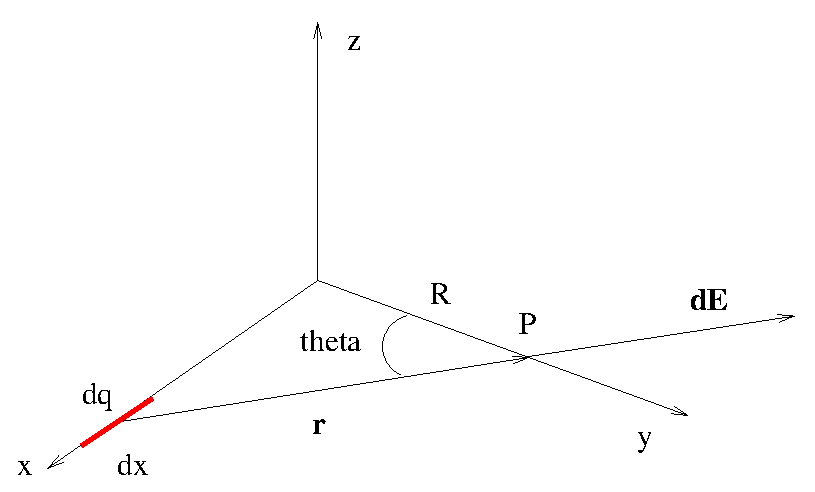
\includegraphics[scale=0.6]{immagini/fisica2/filo_inf}
  \end{figure}
  Im\-ma\-gi\-nia\-mo un filo infinito in coincidenza dell'asse $x$ sul quale sia depositata una densità lineare $\lambda$ uniforme. Il fatto che il filo sia di lunghezza infinita semplifica notevolmente i conti per motivi di simmetria, infatti possiamo dire in qualunque punto lungo l'asse $y$ ci mettiamo di avere metà filo a destra e metà a sinistra. Sia $P$ un punto sull'asse $y$: $P=(0,R,0)$. Consideriamo un elementino del filo $\ud x$, esisterà un altro elementino simmetrico che annulla la componente $x$ del campo; questo per ogni porzione del filo si consideri, in quanto infinito. L'elementino $\ud x$ genera in $P$ un campo $\ud \ve E$. La carica su $\ud x$ è $\ud q=\ud x\lambda$, quindi:
  \[\ud\ve E=\frac{1}{4\pi\varepsilon_0}\frac{\lambda\ud x}{r^3}\ve r\]
  \[\ud E_y=\frac{1}{4\pi\varepsilon_0}\frac{\lambda\ud x}{r^3}r\cos\theta\quad \ud E_x=\ud E_z=0\]
  \[x=R\tan\theta\quad\ud x=R\frac{1}{\cos^2\theta}\ud\theta\quad r=\frac{R}{\cos\theta}\]
  \begin{align*}E_y & =\int\ud E_y=\int_{-\infty}^{+\infty}\frac{1}{4\pi\varepsilon_0}\frac{\lambda\ud x}{r^2}\cos\theta=\frac{\lambda}{4\pi\varepsilon_0}\int_{-\infty}^{+\infty}\frac{\ud x}{r^2}\cos\theta \\
                  & =\frac{\lambda}{4\pi\varepsilon_0}\frac{1}{R}\int_{-\frac{\pi}{2}}^{+\frac{\pi}{2}}\cos\theta\ud\theta=\frac{1}{4\pi\varepsilon_0}\frac{2\lambda}{R}
  \end{align*}
  \[\ve E=\frac{1}{4\pi\varepsilon_0}\frac{2\lambda}{R}\ver{j}\]
  L'ipotesi del filo infinito fisicamente può essere interpretato come $R\ll l$ con $l$ la lunghezza del filo.
\end{Es}
\begin{Es}[Anello]
  \label{es:anello}
  Vogliamo calcolare il valore di $\ve E$ lungo l'asse di un anello con carica totale $q$ uniforme.
  \begin{figure}[htbp]
    \centering
    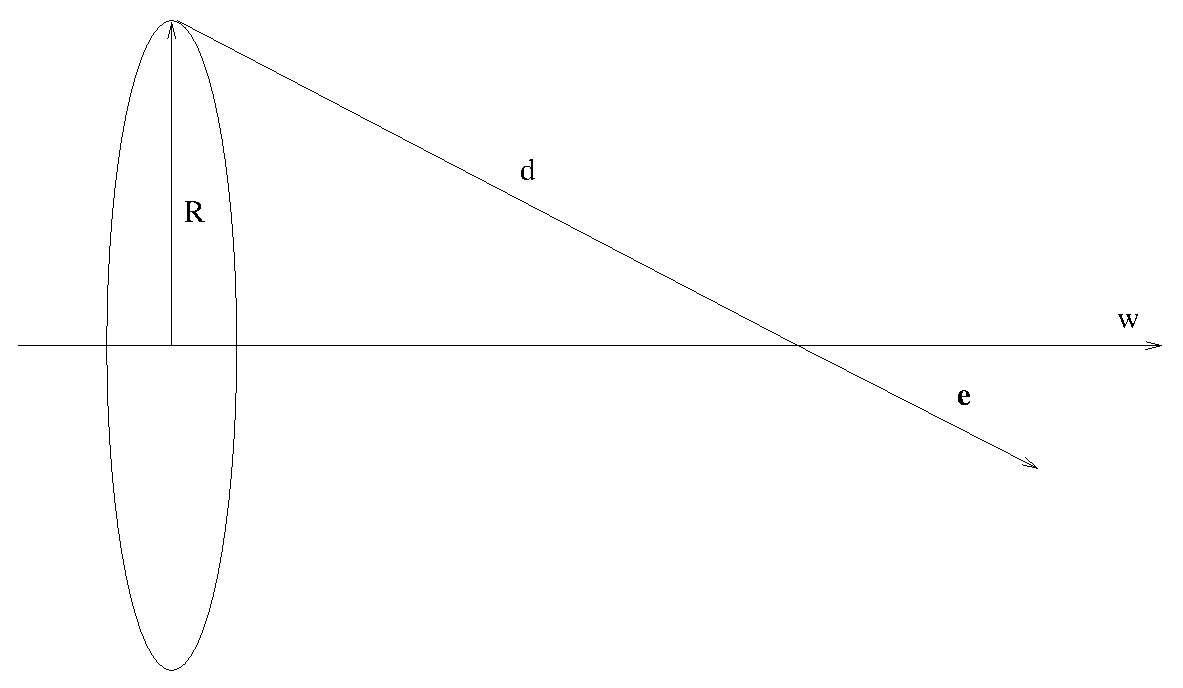
\includegraphics[scale=0.45]{immagini/fisica2/anello}
  \end{figure}
  Data la simmetria del problema usiamo coordinate cilindriche. Per ragioni di simmetria il campo sarà rivolto come il versore $\ver e_w$. Ricaviamo il versore $\ver e$:
  \[\ver e=\cos\alpha\ver e_w+\sin\alpha\ver e_r=\frac{w}{d}\ver e_w+\frac{R}{d}\ver e_r\]
  Sull'elementino infinitesimo dell'anello è depositata la carica $\ud q=\frac{q \ud \theta}{2\pi}$ e $d^2=w^2+R^2$:
  \begin{align*}
    \ve E(0,0,w) & =\int_C\frac{\ud q}{4\pi\varepsilon_0d^2}\ver e                                                                                                                \\
                 & =\int_0^{2\pi}\frac{q}{2\pi}\frac{\ud\theta}{4\pi\varepsilon_0}\frac{1}{R^2+w^2}\ver e                                                                         \\
                 & =\int_0^{2\pi}\frac{q}{2\pi}\frac{\ud\theta}{4\pi\varepsilon_0}\frac{1}{R^2+w^2}\left[\frac{w}{\sqrt{R^2+w^2}}\ver e_w+\frac{R}{\sqrt{R^2+w^2}}\ver e_r\right] \\
                 & =\frac{q}{2\pi}\frac{\ud\theta}{4\pi\varepsilon_0}\frac{1}{R^2+w^2}\left[\frac{w}{\sqrt{R^2+w^2}}\ver e_w\right]\int_0^{2\pi}\ud\theta                         \\
                 & =\frac{q}{4\pi\varepsilon_0}\frac{w}{(R^2+w^2)^{\frac{3}{2}}}\ver e_w                                                                                          \\
  \end{align*}
  Se $w\to +\infty$ coerentemente:
  \[\ve E(0,0,w)\to\frac{q}{4\pi\varepsilon_0}\frac{\ver e_w}{w^2}\]
  cioè come un punto.
\end{Es}
\begin{Es}[Disco]
  \begin{figure}[htbp]
    \centering
    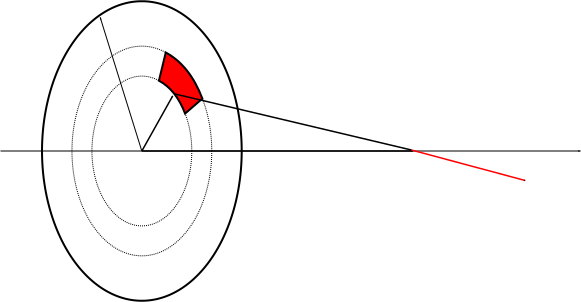
\includegraphics[scale=0.8]{immagini/fisica2/disco}
  \end{figure}
  Consideriamo un disco di raggio $R$ e carica superficiale uniforme $\sigma$. Calcoliamo il campo elettrostatico sull'asse del disco $z$ nel punto $\ve r$. La carica di un elementino infinitesimo sarà:
  \[
    \ud q' = \sigma\ud a = \sigma r'\ud\varphi'\ud r'
  \]
  Il campo che genera sarà:
  \[
    \ud\ve E = \frac{1}{4\pi\varepsilon_0}\ud q'\frac{\ve r-\ve r'}{\norm{\ve r-\ve r'}^3}
  \]
  calcoliamo $\ve r-\ve r'$:
  \begin{gather*}
    \ve r-\ve r'=-r' \ver e_r + z\ver k\\
    \norm{\ve r-\ve r'} = (r'^2+z^2)^{1/2}
  \end{gather*}
  \begin{align*}
    \ve E(0,0,z) & = \frac{1}{4\pi\varepsilon_0}\int \ud q'\frac{\ve r-\ve r'}{\norm{\ve r-\ve r}^3}                          \\
                 & =\frac{1}{4\pi\varepsilon_0}\int \sigma r'\ud r'\ud\varphi'\frac{-r'\ver e_r+z\ver k}{(r'^2+z^2)^{3/2}}    \\
                 & =\frac{\sigma}{4\pi\varepsilon_0}\int\ud r'\int\ud\varphi\frac{-r'^2\ver e_r+r' z\ver k}{(r'^2+z^2)^{3/2}} \\
                 & =\frac{\sigma}{4\pi\varepsilon_0}\int_0^R \ud r'\frac{zr'\ver k}{(r'^2+z^2)^{3/2}}\int_0^{2\pi}\ud\varphi' \\
                 & =\frac{\sigma}{4\pi\varepsilon_0}2\pi z\ver k\int_0^R\frac{r'\ud r'}{(r'^2+z^2)^{3/2}}
  \end{align*}
  questo risultato si può trovare usando l'esempio precedente \ref{es:anello}, in cui $\ve E = \frac{\lambda 2\pi r'}{4\pi\varepsilon_0}\frac{z}{(R^2+z^2)^{3/2}}\ver k$ e $\sigma\ud r=\lambda$, in quando deve essere $\ud q = \sigma\ud a=\lambda r \ud \varphi$. Usando la sostituzione $s = r'^2+z^2$, $\ud s = 2r'\ud r$:
  \begin{align*}
    \ve E(0,0,z) & =\frac{\sigma}{4\pi\varepsilon_0}2\pi z\ver k\int_{z^2}^{R^2+z^2}\frac{\ud s}{2s^{3/2}}                   \\
                 & =\frac{\sigma}{4\pi\varepsilon_0}2\pi z\ver k\left.\frac{-2}{2s^{1/2}}\right|_{z^2}^{R^2+z^2}             \\
                 & =\frac{\sigma}{4\pi\varepsilon_0}2\pi z\ver k\left(\frac{-1}{\sqrt{R^2+z^2}}-\frac{-1}{\sqrt{z^2}}\right) \\
                 & =\frac{\sigma}{2\varepsilon_0} z\left(\frac{1}{|z|}-\frac{1}{\sqrt{R^2+z^2}}\right)\ver k
  \end{align*}
  \begin{figure}[htbp]
    \centering
    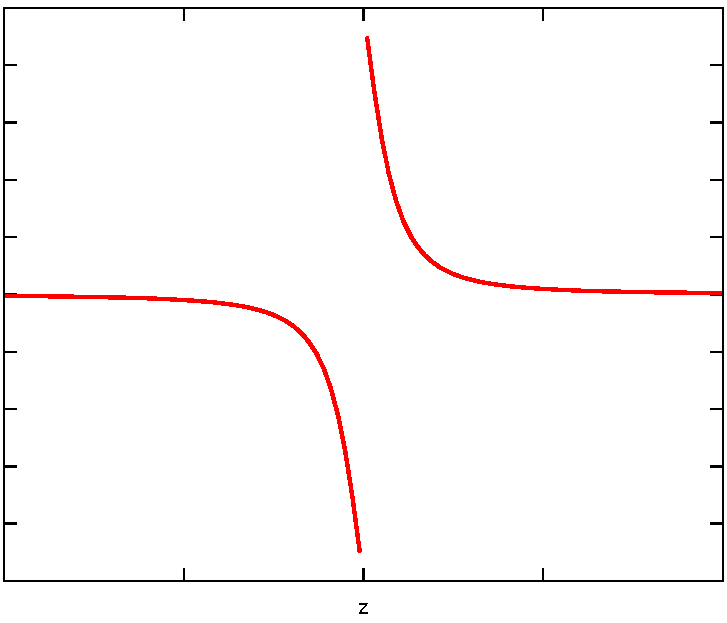
\includegraphics[scale=0.5]{immagini/fisica2/potenziale_disco}
    \caption{Campo elettrico del disco lungo $z$.}
  \end{figure}

  Se sono molto vicino al disco:
  \[
    \lim_{z\to 0^\pm}\ve E(0,0,z)=\lim_{z\to 0^\pm} \frac{\sigma}{2\varepsilon_0} z\left(\frac{1}{|z|}-\frac{1}{\sqrt{R^2+z^2}}\right)\ver k=\pm\frac{\sigma}{2\varepsilon_0}\ver k
  \]
\end{Es}
\begin{Es}[filo finito]
  Consideriamo un filo di lunghezza finita sull'asse $z$ con densità di carica uniforme $\lambda$. Vogliamo trovare il campo elettrostatico lungo l'asse $x$. Un elementino infinitesimo avrà carica $\ud q'=\lambda\ud z'$. e genererà un campo:
  \[
    \ud\ve E(x,0,0) = \frac{\ud q'}{4\pi\varepsilon_0}\frac{\ve r-\ve r'}{\norm{\ve r-\ve r'}^3}
  \]
  con $\ve r=x\ver i$, $\ve r'=z\ver k$, $\ve r-\ve r'=x\ver i-z \ver k$
  \[
    \ve E(x,0,0)=\int\ud \ve E=\frac{\lambda}{4\pi\varepsilon_0}\int\frac{x\ver i-z\ver k}{(x^2+z'^2)^{3/2}}\ud z'
  \]
  per risolvere l'integrale è utile la sostituzione $\tan\gamma=\frac{z'}{x}$:
  \begin{align*}
    \ve E(x,0,0) & =\frac{\lambda}{4\pi\varepsilon_0}\int\frac{x(1+\tan^2\gamma)\ud\gamma}{x^3\left(1+\tan^2\gamma\right)^{3/2}}\left(x\ver i-x\tan\gamma\ver k\right) \\
                 & =\frac{\lambda}{4\pi\varepsilon_0}\frac{1}{x}\int\frac{\ver i-\tan\gamma\ver k}{\left(1+\tan^2\gamma\right)^{1/2}}                                  \\
                 & =\frac{\lambda}{4\pi\varepsilon_0}\frac{1}{x}\int\left(\cos\gamma\ver i-\sin\gamma\ver k\right)
  \end{align*}
  se $z$ varia tra $(z_\text{min},z_\text{max})$, $\gamma$ varia tra $(\gamma_\text{min},\gamma_\text{max})=\arctan\left(\frac{z_\text{max}}{x},\frac{z_\text{min}}{x}\right)$:
  \begin{align*}
    \ve E(x,0,0) & =\frac{\lambda}{4\pi\varepsilon_0}\frac{1}{x}\int_{\gamma_{\text{min}}}^{\gamma_{\text{max}}}\ud\gamma\left(\cos\gamma\ver i-\sin\gamma\ver k\right)                                    \\
                 & =\frac{\lambda}{4\pi\varepsilon_0}\frac{1}{x}\left[\left(\sin\gamma_\text{max}-\sin\gamma_\text{min}\right)\ver i+\left(\cos\gamma_\text{max}-\cos\gamma_\text{min}\right)\ver k\right]
  \end{align*}



\end{Es}


\section{Teorema di Gauss\index{Gauss}\index{teorema!di Gauss}}
\label{teorema_di_gauss}
Immaginiamo una carica puntiforme contenuta in una superficie immaginaria $S$. Per definizione il flusso attraverso $S$ è
\begin{equation}
  \Phi_S(\ve E)=\oint_S\ve E\cdot\ve n\,\ud a
  \label{gauss01}
\end{equation}
Sostituendo nella \eqref{gauss01} il campo elettrico di una carica puntiforme $\ve E=\frac{q}{4\pi\varepsilon_0}\frac{\ve r}{r^3}$ si ottiene:
\begin{align*}
  \Phi_S(\ve E) & =\frac{q}{4\pi\varepsilon_0}\oint_S\frac{\ve r\cdot\ve n}{r^3}\ud a=\frac{q}{4\pi\varepsilon_0}\oint_S\frac{r\cos\theta}{r^3}\ud a                         \\
                & =\frac{q}{4\pi\varepsilon_0}\oint_S\frac{\ud a_0}{r^2}=\frac{q}{4\pi\varepsilon_0}\oint_S\ud\omega=\frac{q}{4\pi\varepsilon_0}4\pi=\frac{q}{\varepsilon_0}
\end{align*}
Infatti $\ud a\cos\theta=\ud a_0$ cioè l'elementino di area infinitesima orientato perpendicolarmente a $\ve E$, mentre $\ud \omega=\frac{\ud a_0}{r^2}$ è per definizione l'angolo solido infinitesimo che sotteso dall'area infinitesima $\ud a_0$.

Questo importante risultato è indipendente dalla geometria della superficie, infatti l'integrale dell'angolo solido su qualsiasi superficie considerata nella sua interezza è $4\pi$ (qui si nota la comodità del sistema razionalizzato). Il risultato poi è valido per qualsiasi forza del tipo $\frac{1}{r^2}$ infatti mentre l'area aumenta col quadrato della distanza, il campo diminuisce col quadrato della distanza e le due cose si semplificano a vicenda.

Se la carica fosse sul bordo della superficie, l'integrale dell'angolo solido sarebbe stato $2\pi$ e quindi:
\[\Phi_S(\ve E)=\frac{1}{2}\frac{q}{\varepsilon_0}\]

Se la carica fosse stata presa all'esterno della superficie allora il flusso attraverso essa sarebbe stato nullo (da una parte entra, dall'altra esce in egual misura), infatti considerando un areola infinitesima $\ud a_1$ o meglio la sua componente normale al campo $\ud a_{01}$ ne corrisponde una $\ud a_{02}$ dove il flusso è uscente. Il flusso netto attraverso queste due superfici è \[\ud\Phi_S(\ve E)=\frac{q}{4\pi\varepsilon_0}\left(\ud\omega_1-\ud\omega_2\right)=0\]
perché $\ud\omega_1=\ud\omega_2$ e perché naturalmente ad ogni areola in cui il campo entra corrisponde una ed una sola areola in cui il campo esce.

Se mettiamo più di una carica puntiforme usiamo il principio di sovrapposizione sul campo, e quindi sul flusso:
\[\ve E=\sum_{i=1}^n \ve E_i\Rightarrow \Phi_S(\ve E)=\oint_S\left(\sum_{i=1}^n\ve E\right)\ve n\,\ud a\]
\begin{Teo}[Gauss per cariche puntiformi]
  Sia $S$ una superficie chiusa e $\{q_i\}_{i=1}^n$ cariche interne ad $S$, definiamo $Q=\sum_{i=1}^n q_i$ allora:
  \begin{equation}
    \Phi_S(\ve E)=\frac{Q}{\varepsilon_0}
  \end{equation}
\end{Teo}
Per una distribuzione di cariche nello spazio $\rho(\ve r)$ basta ricordare che $Q=\int_V\rho(\ve r)\ud v$, quindi:
\begin{Teo}[Gauss]
  Sia $S$ una superficie chiusa, al suo interno vi sia una distribuzione continua di carica $\rho(\ve r)$, allora:
  \begin{equation}
    \Phi_S(\ve E)=\frac{1}{\varepsilon_0}\int_V\rho\,\ud v
  \end{equation}
\end{Teo}
Usando il teorema della divergenza:
\[\Phi_S(\ve E)=\int_S\ve E\cdot\ve n\,\ud a=\int_V\diver\ve E\,\ud v=\frac{1}{\varepsilon_0}\int_V\rho\,\ud v\]
Allora dato che l'integrale vale per qualsiasi superficie e quindi volume, abbiamo:
\begin{equation}
  \diver \ve E(\ve r)=\frac{\rho(\ve r)}{\varepsilon_0}
\end{equation}
che esprime il teorema di Gauss in forma differenziale. Riassumendo:
\begin{equation}
  \ve\nabla\cdot\ve E(\ve r)=\frac{\rho(\ve r)}{\varepsilon_0}\qquad \forall S\,\int_S \ve E\cdot\ve n\,\ud a=\frac{Q}{\varepsilon_0}
\end{equation}
con $Q$ le cariche interne ad $S$.
\begin{Es}[campo sfera piena]
  Sia $B$ una sfera piena di raggio $R$ centrata nell'origine, con densità di carica $\rho$ uniforme. Vogliamo il campo elettrico. Data la simmetria usiamo coordinate sferiche. Dobbiamo dividere lo spazio in due semispazi, uno con $r<R$ e l'altro con $r>R$.
  \[\ve E(r,\theta,\varphi)=E_r\ver e_r+E_\theta\ver e_\theta+E_\varphi \ver e_\varphi=E_r(r)\ver e_r\]
  infatti il campo è radiale e dipende solo dalla distanza dal centro per ragioni di simmetria per rotazioni.
  All'esterno, $r>R$, allora prendiamo una superficie $S$ sferica passante per $P$:
  \[\Phi_S(\ve E)=\oint_S\ve E\cdot\ve n\,\ud a=\oint_S E\ud a=E\oint_S \ud a=4\pi r^2 E\]
  Per il teorema di Gauss:
  \[\Phi_S(\ve E)=\frac{Q}{\varepsilon_0}=\frac{\frac{4}{3}\pi R^3\rho}{\varepsilon_0}\]
  confrontando:
  \[\ve E(\ve r)=\frac{\rho}{3\varepsilon_0}\frac{R^3}{r^2}\ver e_r=\frac{Q^{\text{tot}}}{4\pi\varepsilon_0}\frac{1}{r^2}\ver e_r\]
  Esattamente come se tutta la carica fosse concentrata al centro. All'interno $r<R$, prendiamo una superficie gaussiana $S$ passante per $P$:
  \[\Phi_S(\ve E)=\oint_S\ve E\cdot\ve n\,\ud a=\oint_S E\ud a=E\oint_S \ud a=4\pi r^2 E\]
  Questa volta le cariche contenute nella superficie gaussiana non sono tutte le cariche:
  \[\Phi_S(\ve E)=\frac{Q}{\varepsilon_0}=\frac{\frac{4}{3}\pi r^3\rho}{\varepsilon_0}\]
  confrontando:
  \[\ve E(\ve r)=\frac{\rho}{3\varepsilon_0}r\ve e_r\]
  Il massimo si ha quando $\norm{\ve r}=R$. La funzione che descrive il campo è continua (basta verificarlo per $r=R$), ma ha un punto angoloso.
  \begin{figure}[htbp]
    \centering
    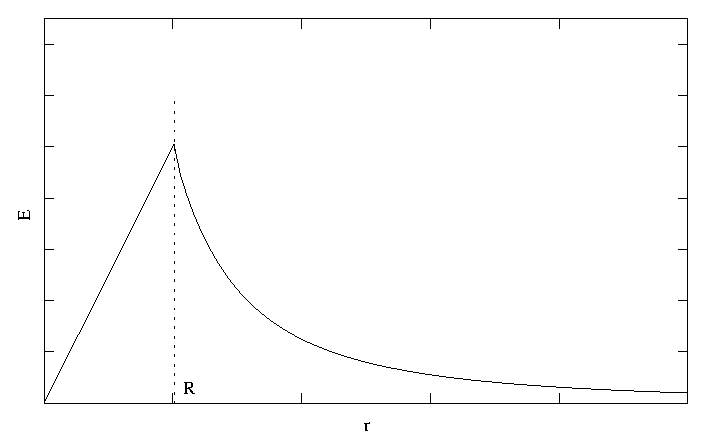
\includegraphics{immagini/fisica2/campo_sfera}
    \caption{Campo di una sfera piena uniformemente carica.}
  \end{figure}
\end{Es}
\begin{Es}[Piano]
  Consideriamo un piano uniformemente carico con distribuzione $\sigma$. Per ragioni di simmetria il campo è perpendicolare al piano. Costruiamo una superficie gaussiana a forma di parallelepipedo, in modo che intersechi il piano. Il flusso non è nullo solo sulle facce parallele al piano. Usando Gauss:
  \begin{align*}
    \Phi_S(\ve E)= & \Phi_{S_1}(\ve E)+\Phi_{S_2}(\ve E)=\int_{S_1}\ve E\cdot\ve n\,\ud a+\int_{S_2}\ve E\cdot\ve n\,\ud a=2EA \\
    =              & \frac{Q}{\varepsilon_0}=\frac{1}{\varepsilon_0}\int_A \sigma\,\ud a=\frac{\sigma A}{\varepsilon_0}
  \end{align*}
  Allora:
  \[E=\frac{\sigma}{2\varepsilon_0}\]
  Notare che non dipende dalla distanza.
\end{Es}
\begin{Es}[condensatore piano\index{condensatore!piano}]
  Consideriamo due lastre molto vicine, che equivale a dire due lastre infinite, parallele con distribuzione $\pm\sigma$. Usando il risultato dell'esempio precedente e del principio di sovrapposizione, ricordando che stiamo sommando quantità vettoriali, possiamo dire che il campo all'esterno è nullo ovunque, mentre tra le due armature è doppio:
  \[E=\frac{\sigma}{\varepsilon_0}\]
  diretto dall'armatura positiva a quella negativa.
\end{Es}
\section{Potenziale elettrostatico\index{potenziale!elettrostatico}}
\begin{figure}[htp]
  \centering
  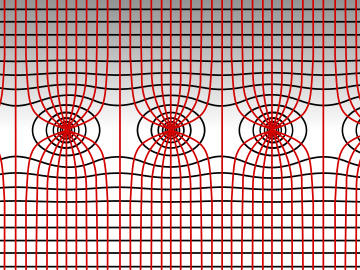
\includegraphics{immagini/fisica2/MWPC}
  \caption{Linee equipotenziali (in nero) e linee di campo (in rosso) per una camera proporzionale a multifili (anodi al centro e catodi sopra e sotto).}
\end{figure}
\begin{Def}[differenza di potenziale]
  La differenza di potenziale tra $P_1$ e $P_2$ è il lavoro svolto per spostare una carica unitaria contro le forze del campo elettrostatico tra i due punti:
  \begin{equation}
    \Delta\varphi=\varphi(P_2)-\varphi(P_1)=\frac{L_{P_1}^{P_2}}{q}
  \end{equation}
\end{Def}
\begin{figure}[htp]
  \centering
  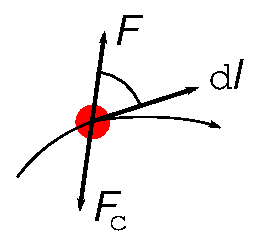
\includegraphics{immagini/fisica2/lavoro_campo}
\end{figure}

Consideriamo un campo $\ve E(\ve r)$ e una carica $q_0$ che si muove su una curva $\Gamma$ congiungente $P_1$ e $P_2$. Dividiamo $\Gamma$ in infinitesimi pezzi $\ud\ve l$, il lavoro elementare compiuto dal campo è
\[\delta L_c=\ve F_c\cdot\ud\ve l\]
Il lavoro totale compiuto dal campo è l'integrale di tutti i lavori elementari:
\[L_c=\int_{P_1}^{P_2}\ve F_c\cdot\ud\ve l=\int_{P_1}^{P_2}q_0\ve E(\ve r)\cdot \ud \ve l\]
Allora noi dovremo svolgere un lavoro $L=-L_c$ perché la nostra forza $\ve F=-\ve F_c$, dunque:
\[\frac{L}{q_0}=-\int_{P_1}^{P_2}\frac{\ve F_c\cdot\ud\ve l}{q_0}=-\int_{P_1}^{P_2}\ve E(\ve r)\cdot\ud\ve l\]
Questa è la differenza di potenziale tra $P_1$ e $P_2$ se si dimostra che non dipende dal cammino, cioè da $\Gamma$.

Consideriamo il campo generato da una carica puntiforme nell'origine, allora per andare da $P_1$ a $P_2$:
\begin{align*}
  \frac{L}{q} & =-\int_{P_1}^{P_2}\ve E\cdot\ud\ve l=-\int_{P_1}^{P_2}\frac{q}{4\pi\varepsilon_0}\frac{\ve r\cdot\ud\ve l}{r^3}=-\frac{q}{4\pi\varepsilon_0}\int_{P_1}^{P_2}\frac{\cos\theta\,\ud l}{r^2} \\
              & =-\frac{q}{4\pi\varepsilon_0}\int_{r_1}^{r_2}\frac{\ud r}{r^2}=\frac{q}{4\pi\varepsilon_0}\left(\frac{1}{r_2}-\frac{1}{r_1}\right)
\end{align*}
Dunque non dipende dal cammino percorso e possiamo dire che:
\begin{Teo}[differenza di potenziale]
  \begin{equation}
    \Delta \varphi=-\int_{P_1}^{P_2}\ve E(\ve r)\cdot\ud\ve l=\varphi(P_2)-\varphi(P_1)
  \end{equation}
\end{Teo}
Possiamo prendere un riferimento $P_0$ e dire che $\varphi(P_0)=k$, allora $\varphi(P_1)$ sarà il lavoro per portare la carica da $P_0$ a $P_1$ e sarà la differenza di potenziale tra $P_0$ e $P_1$; $\varphi(P_2)$ la differenza di potenziale tra $P_0$ e $P_2$. Allora:
\[\Delta \varphi=-\int_{P_1}^{P_2}\ve E\cdot\ud\ve l=-\int_{P_1}^{P_0}\ve E\cdot\ud\ve l-\int_{P_0}^{P_2}\ve E\cdot\ud\ve l=\varphi(P_0)-\varphi(P_1)+\varphi(P_2)-\varphi(P_0)\]
Dunque è indipendente dalla scelta di $P_0$. Per convenzione\footnote{un'altra convenzione è mettere il potenziale della Terra uguale a zero, vedi \eqref{potenziale_terra} a pag.\@\pageref{potenziale_terra}}:
\[\varphi(\infty)=0\]
Quindi per portare una carica dall'infinito:
\[\frac{L}{q_0}=-\int_{\infty}^{P}\ve E\cdot\ud \ve l=\varphi(P)\]
Definiamo il potenziale in un punto (avendo preso come riferimento l'infinito):
\begin{Def}[potenziale]
  \begin{equation}
    \varphi(P)=-\int_{\infty}^P\ve E(\ve r)\cdot\ud\ve l
  \end{equation}
  il lavoro che devo fare per portare la carica unitaria dall'infinito al punto contro le forze del campo.
\end{Def}
\begin{Es}[carica puntiforme nell'origine]
  \[
    \varphi(\ve r)=-\int_{\infty}^r\frac{q}{4\pi\varepsilon_0}\frac{\ve r\cdot\ud\ve l}{r^3}=-\frac{q}{4\pi\varepsilon_0}\int_\infty^r\frac{r}{r^3}\ud r=\frac{q}{4\pi\varepsilon_0}\frac{1}{r}
  \]
\end{Es}
\subsection{Potenziale di qualsiasi distribuzione}
L'espressione del potenziale può essere ricavata notando che $\ve\nabla\frac{1}{r}=-\frac{\ve r}{r^3}$:
\begin{equation}
  \begin{split}
    \ve E &= \frac{1}{\giorgi}\int_V \rho(\ve r')\frac{\ve r-\ve r'}{\norm{\ve r-\ve r'}^3}\,\ud V'\\
    &=-\frac{1}{\giorgi}\int_V \rho(\ve r')\ve\nabla\left(\frac{1}{\ve r-\ve r'}\right)\,\ud V'\\
    &=-\ve\nabla\int_V \frac{1}{\giorgi}\frac{\rho(\ve r')}{\ve r-\ve r'}\,\ud V'\\
    &=-\ve\nabla\varphi(\ve r)
  \end{split}
\end{equation}
per vedere che questo $\varphi$ è proprio il potenziale di prima
\[
  \grad \varphi\cdot\ud\ve l=\ud \varphi=\frac{\delta L}{q}=-\ve E\cdot\ud \ve l\Rightarrow \ve E=-\grad\varphi
\]
In generale, considerando anche cariche puntiformi e superficiali:
\begin{equation}\varphi(\ve r)=\frac{1}{4\pi\varepsilon_0}\left[\sum_i\frac{q_i}{\norm{\ve r-\ve r_i}}+\int_S\frac{\sigma({\ve r}\,')}{\norm{\ve r-\ve r\,'}}\ud a+\int_V\frac{\rho({\ve r}\,')}{\norm{\ve r-{\ve r}\,'}}\ud V\right]\end{equation}
\section{Energia potenziale\index{energia!potenziale!elettrostatica}}
Il potenziale è indipendente dalla carica di prova, l'energia potenziale no. \`E la stessa differenza che c'è tra la forza elettrostatica e il campo elettrostatico, quindi:
\[\Delta W=q\Delta \varphi\]
Rifacendo il discorso per il potenziale: siano $A$ e $B$ due punti, l'integrale è indipendente dal percorso quindi:
\[L_A^B=\int_A^B \ve F\cdot\ud\ve l=-q\int_A^B\ve E\cdot\ud\ve l=q\Delta \varphi=\Delta W=W_B-W_A\]
Per il calcolo abbiamo usato la forza contro le forze del campo, non la forza del campo. Il lavoro a sinistra il lavoro contro le forze del campo, mentre l'energia potenziale a destra è relativa alle forze del campo: ecco perché non c'è il meno.
\subsection{Unità di misura}
Nel SI il potenziale si misura in volt\index{volt}:
\[[\varphi]=\frac{\si{\joule}}{\si{\coulomb}}=\si{\volt}\]
allora essendo $\ve E=-\ve\nabla\varphi$ il campo lo possiamo esprimere in:
\[[\ve E]=[-\ve\nabla\varphi]=\frac{\si{\volt}}{\si{\metre}}\]
\[[U]=\si{\joule}=[q\varphi]=\si{\coulomb\volt}\]
\subsection{Energia di un sistema di cariche\index{energia!di un sistema di cariche}}
Prendiamo una carica $q_1$, portiamola dall'infinito alla posizione $\ve r_1$: non serve compiere lavoro. Ora abbiamo un campo, con un potenziale $\varphi_1(\ve r)$. Prendiamo un'altra carica $q_2$ e portiamola dall'infinito alla posizione $\ve r_2$: dobbiamo compiere un lavoro contro le forze del campo:
\[L_\infty^{\ve r_2}=\int_\infty^{\ve r_2}\ve F\cdot\ud \ve l=-q_2\int_\infty^{\ve r_2} \ve E\cdot\ud \ve l=q_2\varphi_1(\ve r_2)\]
Aggiungiamo una carica $q_3$ in posizione $\ve r_3$, altro lavoro:
\[L_\infty^{\ve r_3}=q_3\varphi_1(\ve r_3)+q_3\varphi_2(\ve r_3)\]
Il lavoro che compiamo va ad accrescere l'energia potenziale del sistema $W$, a questo punto:
\begin{align*}
  W & =q_2\varphi_1(\ve r_2)+q_3\varphi_1(\ve r_3)+q_3\varphi_2(\ve r_3)                                                                  \\
    & =\frac{q_1q_2}{4\pi\varepsilon_0}\frac{1}{\norm{\ve r_1-\ve r_2}}+\frac{q_1q_3}{4\pi\varepsilon_0}\frac{1}{\norm{\ve r_1-\ve r_3}}+
  \frac{q_2q_3}{4\pi\varepsilon_0}\frac{1}{\norm{\ve r_2-\ve r_3}}
\end{align*}
Notiamo che è indifferente l'ordine in cui aggiungiamo le cariche. In generale:
\begin{equation}
  \label{energia_sistema_cariche}
  W=\frac{1}{4\pi\varepsilon_0}\sum_{i=1}^{N}\sum_{j\neq i}^{N}\frac{q_iq_j}{\norm{\ve r_j-\ve r_i}}\cdot\frac{1}{2}=\frac{1}{4\pi\varepsilon_0}\sum_{i<j}\frac{q_iq_j}{\norm{\ve r_j-\ve r_i}}
\end{equation}
Il fattore $\frac{1}{2}$ serve perché altrimenti le coppie sarebbero contate due volte, mentre non conta l'ordine.
\subsubsection{Coppia stesso segno}
Se il campo è generato da una sorgente positiva, allora se muoviamo $+q$ il suo potenziale vale zero all'infinito e vale infinito a zero. Stessa cosa se la sorgente è negativa e la carica esploratrice negativa.
\subsubsection{Coppia segno opposto}
\`E come il caso gravitazionale, essendo in questo caso la forza attrattiva. Il potenziale è massimo e nullo all'infinito, mentre è meno infinito a zero.
\section{Maxwell per l'elettrostatica}
\begin{equation}
  \ve E=-\ve \nabla\varphi
  \label{campo_pot}
\end{equation}
Inoltre:
\[\oint\ve E\cdot\ud\ve l=-\oint\grad\varphi\cdot\ud\ve l=\oint\ud\varphi=0\]
la possiamo scrivere in forma differenziale usando la \eqref{campo_pot}:
\[\rot\ve E=-\rot\grad\varphi=0\]
Abbiamo allora le equazioni di Maxwell per l'elettrostatica in forma integrale:
\begin{subequations}
  \begin{gather}
    \oint\ve E\cdot\ve n\,\ud a=\frac{q}{\varepsilon_0}\\
    \oint\ve E\cdot\ud\ve l=0
  \end{gather}
\end{subequations}
e in forma differenziale:
\begin{subequations}
  \begin{gather}
    \ve\nabla\cdot\ve E(\ve r)=\frac{\rho(\ve r)}{\varepsilon_0}\\
    \ve \nabla\times \ve E(\ve r)=0
  \end{gather}
\end{subequations}
\section{Dipolo\index{dipolo|(}}
\begin{figure}[htbp]
  \centering
  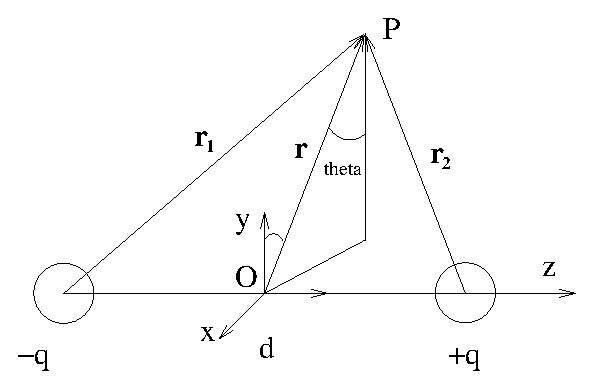
\includegraphics[scale=0.8]{immagini/fisica2/dipolo}
\end{figure}
\subsection{Potenziale}
Consideriamo un dipolo, cioè un sistema di due cariche uguali, con segno opposto, poste ad una distanza $\delta$. Data la simmetria cilindrica usiamo coordinate cilindriche e il potenziale nel punto $P$, individuato dal vettore $\ve r$, non dipende da $\theta$:
\begin{equation}
  \varphi=\varphi(\rho,z)=\frac{1}{4\pi\varepsilon_0}\left\{\frac{-q}{r_1}+\frac{q}{r_2}\right\}
\end{equation}
$r_1$ è la distanza tra il punto $P$ di coordinate $(x,y,z)$ e il punto $A$ di coordinate $(0,0,\delta/2)$, quindi:
\[
  r_2 = \norm{P-A} = \sqrt{x^2+y^2+(z-\delta/2)^2}=\sqrt{\rho^2+(z-\delta/2)^2}
\]
e allora:
\begin{equation}
  \frac{1}{4\pi\varepsilon_0}\left\{\frac{-q}{\sqrt{\left(z+\frac{\delta}{2}\right)^2+\rho^2}}+\frac{q}{\sqrt{\left(z-\frac{\delta}{2}\right)^2+\rho^2}}\right\}
  \label{dipolo01}
\end{equation}
I due denominatori della \eqref{dipolo01} li possiamo sviluppare:
\[\left(z^2+\rho^2+\delta z+\frac{\delta^2}{4}\right)^{-\frac{1}{2}}=\left(z^2+\rho^2\right)^{-\frac{1}{2}}\left(1+\frac{\delta z}{\rho^2+z^2}+\frac{\delta^2}{4\left(\rho^2+z^2\right)}\right)^{-\frac{1}{2}}\]
\[\left(z^2+\rho^2-\delta z+\frac{\delta ^2}{4}\right)^{-\frac{1}{2}}=\left(z^2+\rho^2\right)^{-\frac{1}{2}}\left(1-\frac{\delta z}{\rho^2+z^2}+\frac{\delta^2}{4\left(\rho^2+z^2\right)}\right)^{-\frac{1}{2}}\]
se vogliamo considerare $\ve E$ a grande distanza equivale a dire che $\delta$ deve essere molto piccolo, quindi il termine $\delta^2$ non lo consideriamo. Ricordiamo lo sviluppo binomiale:
\[\left(1+x\right)^\alpha=1+\alpha x+\frac{\alpha\left(\alpha-1\right)}{2}x^2+\cdots\]
Allora usando solo il primo ordine:
\[\left(z^2+\rho^2+\delta z+\frac{\delta^2}{4}\right)^{-\frac{1}{2}}\simeq\left(z^2+\rho^2\right)^{-\frac{1}{2}}\left(1-\frac{1}{2}\frac{\delta z}{\rho^2+z^2}\right)\]
\[\left(z^2+\rho^2-\delta z+\frac{\delta^2}{4}\right)^{-\frac{1}{2}}\simeq\left(z^2+\rho^2\right)^{-\frac{1}{2}}\left(1+\frac{1}{2}\frac{\delta z}{\rho^2+z^2}\right)\]
sostituendo nella \eqref{dipolo01}:
\begin{align*}
  \varphi & =\varphi(\rho,z)=\frac{1}{4\pi\varepsilon_0}\frac{1}{\sqrt{\rho^2+z^2}}\left\{-q\left(1-\frac{1}{2}\frac{\delta z}{\rho^2+z^2}\right)+q\left(1+\frac{1}{2}\frac{\delta z}{\rho^2+z^2}\right)\right\} \\
          & =\frac{q}{4\pi\varepsilon_0}\frac{\delta z}{\left(\rho^2+z^2\right)^\frac{3}{2}}
\end{align*}
che è l'espressione del potenziale del dipolo in coordinate cilindriche. Ma $\sqrt{z^2+\rho^2}=\norm{\ve r}$, definiamo $\ve p=\pm |q|\delta \ver e_z$, con il verso tale che sia diretto dalla carica negativa a quella positiva, momento del dipolo. Essendo $\ve r=\rho\ver e_r+z\ver e_z$ allora $\ve p\cdot\ve r=q\delta z$. In funzione di $\ve r$:
\[\varphi=\varphi(\ve r)=\frac{1}{4\pi\varepsilon_0}\frac{\ve p\cdot\ve r}{{\norm{\ve r}}^3}\]
Dunque il potenziale decresce con $r^2$. Usando $\ve\nabla\left(\frac{1}{r}\right)=-\frac{\ve r}{r^3}$, lo possiamo anche scrivere come:
\begin{equation}
  \varphi(\ve r)=-\frac{1}{4\pi\varepsilon_0}\ve p\cdot\ve\nabla\left(\frac{1}{r}\right)
\end{equation}
oppure come:
\begin{equation}
  \varphi(\ve r)=-\ve p\cdot\ve\nabla\Phi_0
\end{equation}
con $\Phi_0$ il potenziale sulla carica($\frac{1}{4\pi\varepsilon_0}\frac{1}{r}$). Usando le coordinate cartesiane, $\ve r=x\ver \imath+y\ver \jmath+z\ver k$, $\ve p=p\ver k$:
\begin{equation}
  \varphi(x,y,z)=\frac{1}{4\pi\varepsilon_0}\frac{pz}{\left(x^2+y^2+z^2\right)^\frac{3}{2}}
\end{equation}\index{potenziale!elettrostatico!del dipolo}
\subsubsection{Altra dimostrazione}
Immaginiamo una carica $q$ nell'origine, allora il suo potenziale è $\varphi_0\left(\ve r\right)=\frac{1}{4\pi\varepsilon_0}\frac{q}{r}$
spostiamo di $\Delta\ve r=\frac{\ve\delta}{2}$ la carica, allora:
\[\varphi_+\left(\ve r\right)=\varphi_0(\ve r-\Delta \ve r)\simeq\varphi_0-\ve\nabla\varphi_0\cdot\Delta\ve r=\frac{1}{4\pi\varepsilon_0}\frac{q}{r}-\frac{1}{4\pi\varepsilon_0}q\ve\nabla\left(\frac{1}{r}\right)\cdot\frac{\ve\delta}{2}\]
La stessa cosa la possiamo fare con una carica $-q$ e spostarla dall'altra parte $-\Delta\ve r$:
\[\varphi_-\left(\ve r\right)=-\varphi_0(\ve r+\Delta \ve r)\simeq-\varphi_0-\ve\nabla\varphi_0\cdot\Delta\ve r=-\frac{1}{4\pi\varepsilon_0}\frac{q}{r}-\frac{1}{4\pi\varepsilon_0}q\ve\nabla\left(\frac{1}{r}\right)\cdot\frac{\ve\delta}{2}\]
Essendo $\delta\ll r$ allora è una buona approssimazione. Il potenziale totale:
\[\varphi\left(\ve r\right)=\varphi_++\varphi_-=-\frac{1}{4\pi\varepsilon_0}q\ve\nabla\left(\frac{1}{r}\right)\cdot\ve\delta=-\frac{1}{4\pi\varepsilon_0}\ve p\cdot\ve\nabla\left(\frac{1}{r}\right)\]


\subsection{Campo elettrostatico\index{campo!elettrostatico!del dipolo}}
Usando $\ve E=-\grad\varphi$:
\begin{align}
  \label{eq:E_dipolo}
  E_x & =-\frac{\partial\varphi}{\partial x}=\frac{3pz}{4\pi\varepsilon_0}\frac{x}{\left(x^2+y^2+z^2\right)^\frac{5}{2}}=\frac{3pz}{4\pi\varepsilon_0}\frac{x}{r^5}=\frac{3(\ve p\cdot \ve r)}{\giorgi}\left[\frac{\ve r}{r^5}\right]_x \\
  E_y & =-\frac{\partial\varphi}{\partial y}=\frac{3pz}{4\pi\varepsilon_0}\frac{y}{\left(x^2+y^2+z^2\right)^\frac{5}{2}}=\frac{3pz}{4\pi\varepsilon_0}\frac{y}{r^5}=\frac{3(\ve p\cdot \ve r)}{\giorgi}\left[\frac{\ve r}{r^5}\right]_y \\
  E_z & =-\frac{\partial\varphi}{\partial z}=\frac{p}{\giorgi}\left(\frac{3z^2}{r^5}-\frac{1}{r^3}\right)=\frac{3(\ve p\cdot \ve r)}{\giorgi}\left[\frac{\ve r}{r^5}\right]_z-\frac{1}{\giorgi}\left[\frac{\ve p}{r^3}\right]_z
\end{align}
definiamo:
\[E_\perp=\sqrt{E_x^2+E_y^2}=\frac{3pz}{4\pi\varepsilon_0}\frac{1}{r^{5}}\sqrt{x^2+y^2}\]
allora:
\[E=\sqrt{E_z^2+E_\perp^2}=\frac{1}{4\pi\varepsilon_0}\frac{p}{r^3}\sqrt{\frac{3z^2}{r^2}+1}=\frac{1}{4\pi\varepsilon_0}\frac{p}{r^3}\sqrt{3\cos^2\theta+1}\]
in forma vettoriale:
\begin{equation}
  \label{eq:campo_dipolo}
  \ve E(\ve r)=\frac{1}{4\pi\varepsilon_0}\left\{3\left(\ve p\cdot\ve r\right)\frac{\ve r}{r^5}-\frac{\ve p}{r^3}\right\}\end{equation}
Esso decresce con $r^3$ ed è solenoidale, cioè le linee del campo si chiudono. Da questa discende che il flusso su una superficie che racchiude il dipolo è nullo.
\subsection{Energia potenziale\index{energia!potenziale!del dipolo}}
Mettiamo un dipolo in un campo elettrico $\ve E$ esterno. Assumiamo che le due cariche non si muovano. Dove c'è la carica $-q$ ci sia un potenziale esterno $\varphi_A$, nell'altra $\varphi_B$. L'energia potenziale è la somma dell'energia potenziale delle due cariche:
\[W=W_B+W_A=q(\varphi_B-\varphi_A)\]
Calcoliamo il potenziale $\varphi_B$ sviluppando $\varphi_A$ nell'intorno di $\varphi_A$:
\[\varphi_B\simeq\varphi_A+\ve\nabla\varphi\cdot\ve\delta\]
Allora l'energia diventa:
\[W=q\left(\varphi_A+\ve\nabla\varphi\cdot\ve\delta-\varphi_A\right)=q\ve\delta\cdot\ve\nabla\varphi=-\ve p\cdot\ve E\]
Si deduce che la posizione di equilibrio stabile, che corrisponde all'energia minima, si ha quando $\ve p//\ve E$ cioè quando il dipolo è orientato come il campo elettrico esterno. Quando $\ve p$ è antiparallelo al campo elettrico si ha un equilibrio instabile.
\subsection{Forza\index{forza!sul dipolo}}
\label{forza_dipolo100}
\[\ve F=-\ve\nabla W=\ve\nabla\left(\ve p\cdot\ve E\right)=\left(\ve p\cdot\ve\nabla\right)\ve E\]
per esempio:
\[F_x=\left(p_x\frac{\partial E_x}{\partial x}+p_y\frac{\partial E_x}{\partial y}+p_z\frac{\partial E_x}{\partial z}\right)\]
quindi se il campo elettrico esterno è omogeneo allora non c'è forza sul dipolo.
\subsection{Momento\index{momento!sul dipolo}}
\begin{figure}[htbp]
  \centering
  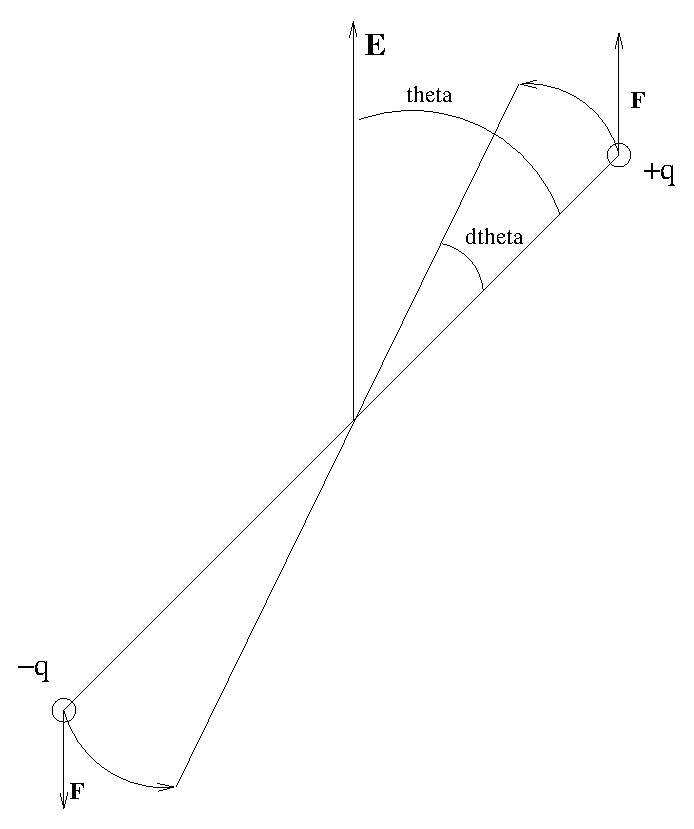
\includegraphics[scale=0.5]{immagini/fisica2/dipolo_mom}
\end{figure}
Il lavoro per far ruotare il sistema di $\ud\theta$ è
\[\delta L=-M\ud\theta\]
notare che $\theta$ diminuisce, quindi la sua variazione è negativa. Essendo il sistema isolato il lavoro compiuto deve tramutarsi in variazione di energia potenziale:
\[\ud W=\delta L=M\ud\theta\]
Allora:
\[M=\frac{\ud W}{\ud\theta}=\frac{-pE\cos\theta}{\ud\theta}=pE\sin\theta\]
\[\ve M=\ve p\times\ve E\]
che fa ruotare il dipolo fino alla posizione di equilibrio. Questa relazione può essere calcolata semplicemente dalla definizione di momento torcente:
\[
  \ve M = \ve r_+\times \ve F_+ + \ve r_-\times\ve F_- = q(\ve r_+-\ve r_-)\times \ve E=\ve p\times\ve E
\]

\subsection{Interazione dipolo-dipolo}
Consideriamo due dipoli $\ve p_1$ e $\ve p_2$. Vogliamo sapere come interagiscono. Calcoliamo prima l'energia potenziale del sistema. Il campo generato del primo dipolo è:
\[
  \ve E_1 = \frac{1}{\giorgi}\left(3(\ve p_1\cdot \ve r)\frac{\ve r}{r^5}-\frac{\ve p_1}{r^3}\right)
\]
quindi l'energia di interazione è:
\[
  U = -\ve E_1\cdot \ve p_2 = \frac{1}{\giorgi}\left(3\frac{(\ve p_1\cdot \ve r)(\ve p_2\cdot \ve r)}{r^5}-\frac{\ve p_1\cdot\ve p_2}{r^3}\right)
\]
che varia come $\frac{1}{r^3}$. Quest'interazione è quella che si verifica tra molecole neutre ma polari, che presentano un momendo di dipolo, come l'acqua.
\index{dipolo|)}
\section{Sviluppo in multipoli\index{multipoli|(}\index{sviluppo!in multipoli|(}}
Il multipolo è un sistema formato da diverse cariche. Ci interessa sapere come si comporta $\varphi$ a grande distanza. Una distribuzione di cariche può essere approssimata a grande distanza da sovrapposizione di multipoli.
\subsection{Distribuzione di carica}
Immaginiamo una distribuzione di carica nello spazio con densità $\rho(x,y,z)$. Sia l'origine all'interno della distribuzione. Il potenziale totale è
\begin{equation}
  \varphi(\ve r)=\frac{1}{4\pi\varepsilon_0}\int_V\frac{\rho(\ve r\,')\ud v}{\norm{\ve r-\ve r\,'}}
  \label{multipolo_01}
\end{equation}
\begin{center}
  $
    \xymatrix{
      &&C&&&\\
      \\
      \\
      A\ar[rruuu]^{\ve r}\ar[rrrrr]^{\ve r\,'}&&&&&B\ar[llluuu]_{\ve r-\ve r\,'}
    }$\end{center}
Usando il teorema dei coseni possiamo scrivere:
\[\norm{\ve r-\ve r\,'}=\sqrt{r^2+r'^2-2\ve r\cdot \ve r\,'}=r\sqrt{1+\frac{r'^2}{r^2}-\frac{2\ve r\cdot \ve r\,'}{r^2}}\]
Ricordando che:
\[(1+\varepsilon)^{-\frac{1}{2}}=1-\frac{1}{2}\varepsilon+\frac{3}{8}\varepsilon^2+\cdots\]
si ha:
\begin{align*}
  {\norm{\ve r-\ve r\,'}}^{-1}= & \frac{1}{r}\left(1+\frac{r'^2}{r^2}-\frac{2\ve r\cdot \ve r\,'}{r^2}\right)^{-\frac{1}{2}}                                                                                                                                                                                                                                                                                                                                             \\
  =                             & \frac{1}{r}\left\{1+\frac{\ve r\cdot\ve r\,'}{r^2}-\frac{1}{2}\frac{r'^2}{r^2}+\frac{3}{8}\left[\frac{2\ve r\cdot\ve r\,'}{r^2}-\frac{r'^2}{r^2}\right]^2+o\left(\frac{r'}{r}\right)^2\right\}                                                                                                                                                                                                                                         \\
  =                             & \frac{1}{r}\left\{\underbrace{1}_{\sim 1}+\underbrace{\frac{\ve r\cdot\ve r\,'}{r^2}}_{\sim x}-\underbrace{\frac{1}{2}\frac{r'^2}{r^2}}_{\sim x^2}+\underbrace{\frac{3}{8}\left(\frac{r'}{r}\right)^4}_{\sim x^4}-\underbrace{\frac{3}{8}\left(\frac{r'}{r}\right)^2\frac{\ve r\cdot \ve r'}{r^3}}_{\sim x^3}+\underbrace{\frac{3}{2}\frac{(\ve r\cdot \ve r')}{r^4}}_{x^2}+\underbrace{o\left(\frac{r'}{r}\right)^2}_{o(x^2)}\right\} \\
  \simeq                        & \frac{1}{r}+\frac{\ve r\cdot\ve r\,'}{r^3}+\frac{1}{2}\left[-\frac{r'^2}{r^3}+\frac{3\left(\ve r\cdot\ve r\,'\right)^2}{r^5}\right]                                                                                                                                                                                                                                                                                                    \\
\end{align*}
Nell'ultimo passaggio abbiamo considerato che $r\gg r'$. Sostituendo l'ultimo risultato nella \eqref{multipolo_01} si ottiene:
\begin{multline}
  \label{multipolo02}
  \varphi(\ve r)\simeq\frac{1}{4\pi\varepsilon_0}\left\{\frac{1}{r}\int_V\rho(\ve r\,')\,\ud v+\frac{\ve r}{r^3}\cdot\int_V\rho(\ve r\,')\ve r\,'\,\ud v+\right.\\
  \left.+\frac{1}{2}\int_V\rho(\ve r\,')\left[\frac{3\left(\ve r\cdot\ve r\,'\right)^2}{r^5}-\frac{r'^2}{r^3}\right]\,\ud v\right\}
\end{multline}
Analizziamo i termini della \eqref{multipolo02}. Il primo:
\[\frac{1}{4\pi\varepsilon_0}\frac{1}{r}\int_V\rho(\ve r\,')\,\ud v=\frac{1}{4\pi\varepsilon_0}\frac{Q}{r}\]
è il potenziale di un monopolo, cioè il potenziale di un punto in cui è accumulata tutta la carica della distribuzione. A grande distanza è un'approssimazione accettabile. Il secondo termine corregge il precedente:
\[\frac{1}{4\pi\varepsilon_0}\frac{\ve r}{r^3}\cdot\int_V\rho(\ve r\,')\ve r\,'\,\ud v\]
è il potenziale di un dipolo, infatti possiamo definire:
\[\ve p=\int_V\rho(\ve r\,')\ve r\,'\ud v\]
momento di dipolo della distribuzione di carica. Gli altri termini sono i potenziali di quadripolo, ottupolo, \ldots Notare che:
\begin{equation}
  \ve\delta=\frac{\ve p}{|q|}=\frac{\int_V\rho(\ve r\,')\ve r\,'\ud v}{|q|}
\end{equation}
individua il centro di \index{centro!di carica}carica.\index{sviluppo!in multipoli|)}\index{multipoli|)}
\begin{Es}[Doppio anello]
  Siano due anelli sottili di raggio $R$ nel piano $x$--$y$ ad altezza $z=\pm\frac{d}{2}$ e con il centro sull'asse $z$. Gli anelli sono uniformemente carichi con densità lineare $\pm\lambda$. Calcolare il campo elettrico totale lungo l'asse $z$, fare un'approssimazione per $|z|\gg d,R$.
  \begin{figure}[htbp]
    \centering
    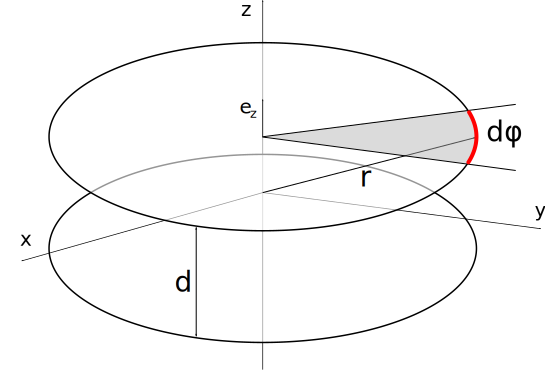
\includegraphics[scale=0.5]{immagini/fisica2/due_anelli_schema}
    % due_anelli_schema.pdf: 436x297 pixel, 72dpi, 15.38x10.48 cm, bb=0 0 436 297
  \end{figure}

  Il campo elettrico può essere trovato con il principio di sovrappossizione, calcolando separatamente i campi generati da ciascun anello. Come calcolato nell'esempio \ref{es:anello} il campo elettrico generato da un anello nell'origine lungo il suo asse è:
  \begin{align*}
    \ve E_0(0,0,z) & =\frac{q}{4\pi\varepsilon_0}\frac{z}{(R^2+z^2)^{\frac{3}{2}}}\ver e_z      \\
                   & =\frac{\lambda R}{2\varepsilon_0}\frac{z}{(R^2+z^2)^{\frac{3}{2}}}\ver e_z
  \end{align*}
  quindi il campo elettrico generato dai due anelli è:
  \begin{align*}
    \ve E(0,0,z) & =\ve E_{+\frac{d}{2}}+\ve E_{-\frac{d}{2}} \\
                 & =\frac{\lambda R}{2\varepsilon_0}\left\{
    \frac{z-\frac{d}{2}}{\left[R^2+(z-\frac{d}{2})^2\right]^{\frac{3}{2}}}
    -\frac{z+\frac{d}{2}}{\left[R^2+(z+\frac{d}{2})^2\right]^{\frac{3}{2}}}\right\}\ver e_z
  \end{align*}
  Per ottenere un'appossimazione per $|z|\gg d,R$ possiamo fare uno sviluppo di Taylor:
  \begin{multline*}
    \frac{z-\frac{d}{2}}{\left[R^2+(z-\frac{d}{2})^2\right]^{\frac{3}{2}}}
    =\frac{z}{|z|^3}\frac{(1-\frac{d}{2z})}{\left[\underbrace{\left(\frac{R}{z}\right)^2}_{\simeq 0}+\left(1-\frac{d}{2z}\right)^2\right]^{3/2}}\\
    \simeq\frac{\sgn{z}}{z^2}\left(1-\frac{d}{2z}\right)\left(1+\frac{3d}{2z}\right)
    \simeq\frac{\sgn{z}}{z^2}\left(1+\frac{d}{z}\right)
  \end{multline*}
  La semplificazione $\left(\frac{R}{z}\right)^2\simeq 0$ e anche quella nell'ultimo passaggio sono giustificate dal fatto che la nostra espanzione è al primo grado. Quindi la nostra approssimazione per il campo elettrostatico:
  \[
    \ve E(0,0,z) \simeq \frac{\lambda R}{2\varepsilon_0}\frac{\sgn{z}}{z^2}\left\{\left(1+\frac{d}{z}\right)-\left(1-\frac{d}{z}\right)\right\}\ver e_z
    = \frac{\lambda R}{\varepsilon_0}\frac{d}{|z|^3}\ver e_z
  \]
  Notiamo che la dipendenza da $\frac{1}{r^3}$ è tipica dei dipoli \eqref{eq:campo_dipolo}, infatti il sistema è approssimabile con un dipolo che punta dall'anello negativo a quello positivo:
  \[
    \ve p = \int_\Gamma \ve r\,\ud q = \int_{\Gamma_+} \left\{\frac{d}{2}\ver e_z+R\ver u_r\right\}\left(\lambda R\ud\phi\right) + \int_{\Gamma_-} \left\{-\frac{d}{2}\ver e_z+R\ver u_r\right\}\left(-\lambda R\ud\phi\right)
  \]
  spezzando gli integrali le parti che contengono $\ver u_r$ si annullano, in quando la somma di tutti i versori radiali, al variare dell'angolo $\phi$ fa il vettore nullo.
  \[
    \ve p = 2\pi\lambda R d\ver e_z
  \]
  questo vuol dire che il nostro sistema è assimilabile a un sistema di due cariche di carica $\pm 2\pi\lambda R $ e distanti $d$, quindi come se fossero messe nel centro degli anelli. Usando l'espressione del campo elettrico generato da un dipolo \eqref{eq:campo_dipolo}:
  \begin{align*}
    \ve E(0,0,z) & = \frac{1}{\giorgi}\left\{3(\ve p\cdot\ve r)\frac{\ve r}{r^5}-\frac{\ve p}{r^3}\right\}                                                  \\
                 & = \frac{1}{\giorgi}\left\{3(2\pi\lambda R d\ver e_z\cdot z\ver e_z)\frac{z\ver e_z}{|z|^5}-\frac{2\pi\lambda R d\ver e_z}{|z|^3}\right\} \\
                 & = \frac{\lambda R}{\varepsilon_0}\frac{d}{|z|^3}\ver e_z
  \end{align*}
  avendo usato $\ve r=z\ver e_z$ e quindi $r = |z|$.
  \begin{figure}[htbp]
    \centering
    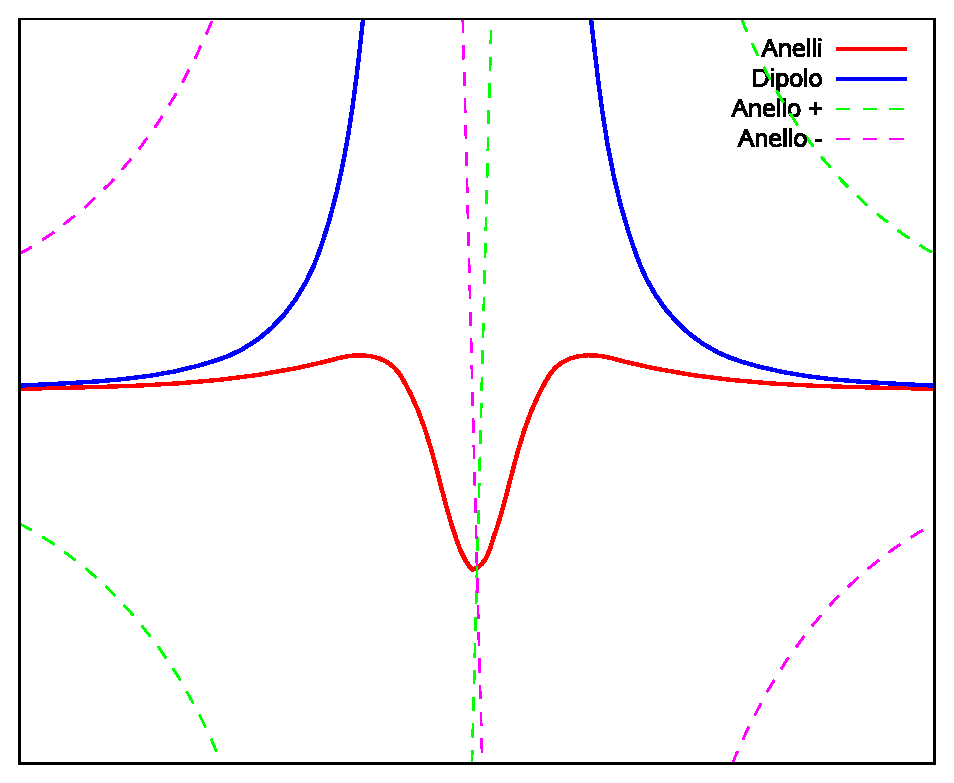
\includegraphics[scale=0.5]{immagini/fisica2/due_anelli}
    % due_anelli.pdf: 480x384 pixel, 72dpi, 16.93x13.55 cm, bb=0 0 480 384
    \caption{campo elettrostatico di due anelli lungo l'asse $z$ (esatto, approssimazione di dipolo e anelli singoli).}
  \end{figure}
\end{Es}
\begin{Es}[Doppio anello 2]
  Calcolare il lavoro che deve essere fatto dall'esterno per portare una carica $e$ da un punto infinitamente lontano all'origine. Calcolare il lavoro che dev'essere fatto per portare un dipolo $\ve p$ con il verso lungo l'asse $z$ da un punto infinitamente lontano all'origine.

  Il lavoro fatto dall'esterno può calcolare come variazione dell'energia potenziale:
  \[
    L_\text{ext} = e(\varphi(0)-\varphi(\infty))
  \]
  Per valutare il potenziale al posto di fare la derivata del campo lo si può calcolare dalla definizione. Il potenziale generato da una spira sull'asse è:
  \[
    \varphi_0 = \frac{1}{\giorgi}\int\frac{\ud q}{\norm{\ve r - \ve r'}} = \frac{1}{\giorgi}\int_0^{2\pi}\frac{\lambda R\ud\phi}{\left[R^2+\left(z-\frac{d}{2}\right)^2\right]^{1/2}}=\frac{\lambda R}{2\varepsilon_0}\frac{1}{\sqrt{z^2+R^2}}
  \]
  quindi il potenziale dei due anelli:
  \[
    \varphi = \varphi_{+\frac{d}{2}} - \varphi_{-\frac{d}{2}} = \frac{\lambda R}{2\varepsilon_0}\left\{\frac{1}{\sqrt{\left(z-\frac{d}{2}\right)^2+R^2}}-\frac{1}{\sqrt{\left(z+\frac{d}{2}\right)^2+R^2}}\right\}
  \]
  poiché $\varphi(0)=0$ e $\varphi(\infty)=0$ il lavoro è nullo. Alla conclusione che $\varphi(0)=0$ ci si poteva arrivare anche con ragionamenti sulla simmetria del sistema. Infatti sicuramente $\varphi_0(z) = \varphi(-z)$ quindi
  \[
    \begin{aligned}
      \varphi(z=0) & = \left[\varphi_0(z+d/2)-\varphi_0(z-d/2)\right]_{z=0}               \\
                   & = \varphi_0(d/2)-\varphi_0(-d/2) = \varphi_0(d/2)-\varphi_0(d/2) = 0
    \end{aligned}
  \]


  Il lavoro fatto per spostare il dipolo si può fare in maniera analoga, ricordando che l'energia potenziale di un dipolo che interagisce con un campo elettromagnetico è $-\ve p\cdot \ve E$.
  \begin{align*}
    W(0) & = -\ve p\cdot \frac{\lambda R}{2\varepsilon_0}\left\{
    \frac{z-\frac{d}{2}}{\left[R^2+\left(z-\frac{d}{2}\right)^2\right]^{\frac{3}{2}}}
    -\frac{z+\frac{d}{2}}{\left[R^2+\left(z+\frac{d}{2}\right)^2\right]^{\frac{3}{2}}}\right\}_{z=0}\ver e_z \\
         & = p\frac{\lambda R}{2\varepsilon_0}
    \frac{d}{\left[R^2+\left(\frac{d}{2}\right)^2\right]^{\frac{3}{2}}}
  \end{align*}
  essendo $W(\infty)=0$ questo è già il lavoro.
\end{Es}



\chapter{Elettrostatica nei conduttori\index{elettrostatica!nei conduttori}}
\minitoc
\section{Conduttori ed isolanti\index{conduttori}\index{isolanti}}
Dal punto di vista elettrico i materiali possono essere divisi in due categorie:
\begin{description}
  \item[conduttori] hanno molte cariche elettriche libere, una nuvola elettronica con densità constante in condizioni standard;
  \item[isolanti] hanno atomi e molecole molto legati tra di loro che atomi tendono a deformarsi sotto l'effetto di un campo elettrico;
\end{description}
I materiali si caratterizzano per tre costanti:
\begin{itemize}
  \item conducibilità elettrica $\sigma$, descrive la risposta dei suoi elettroni soggetti a un campo elettrico esterno;
  \item costante dielettrica $\varepsilon$;
  \item permeabilità magnetica $\mu$;
\end{itemize}

\section{Carica nei conduttori}
Se carichiamo un conduttore gli elettroni dopo una frazione di tempo trovano una condizione di equilibrio, in cui non agisce nessuna forza netta,  e quindi il campo elettrostatico all'interno del conduttore deve essere nullo. In realtà questa non è una grande dimostrazione, un'altra soluzione potrebbe essere che in presenza di conduttori le cariche non stanno mai ferme.

Se viene applicato un campo elettrico esterno al conduttore, allora le cariche al suo interno si muoveranno creando un campo elettrico indotto che si oppone a quello esterno. Il movimento delle cariche continuerà finché il campo elettrico indotto non sarà uguale e contrario a quello esterno. In questo modo la somma del campo elettrico esterno e di quello indotto è nullo. Questo processo è praticamente istantaneo. Ovviamente il campo elettrico esterno può essere non nullo.

Essendo il campo il gradiente del potenziale allora se il campo è nullo il potenziale è costante e quindi il conduttore è un corpo equipotenziale e in particolare la sua superficie è equipotenziale.

Il campo elettrostatico all'esterno è ortogonale alla superficie essendo essa una superficie equipotenziale, inoltre se esso avesse una componente tangenziale le cariche al suo interno si muoverebbero.

Usando il teorema di Gauss, con superfici gaussiane che tendono al bordo scopriamo che all'interno non ci possono essere cariche, allora per la conservazione della carica esse sono sul bordo. Con la versione differenziale $\diver\ve E=\rho$ si ottiene la stessa conclusione più rapidamente. La carica netta deve essere sulla superficie.
\section{Induzione elettrostatica}
\begin{Def}[Induzione elettrostatica\index{induzione elettrostatica}]
  L'induzione elettrostatica è quel fenomeno per cui in presenza di un campo elettrico esterno le cariche libere in un conduttore si ridistribuiscono.
\end{Def}
Se mettiamo un conduttore in uno spazio in cui è presente un campo elettrico $\ve E_\text{ext}$ gli elettroni al suo interno si muovono in senso opposto ad $\ve E_\text{ext}$. In questo modo creano un accumulo di cariche che a sua volta crea un campo elettrico indotto dalla carica migrata $\ve E_i$. In pochissimo tempo gli elettroni arrivano ad un a posizione di equilibrio in cui:
\[\ve E=\ve E_i+\ve E_\text{ext}=0\]
Possiamo allora affermare che (a parte il brevissimo istante in cui le cariche creano raggiungono l'equilibrio) il campo elettrico totale all'interno di un conduttore ideale è nullo. A causa della migrazione della carica all'interno del conduttore questo si attrarrà con la carica. Anche il campo esterno risulta deformato dalla nuova distribuzione di cariche e a grande distanza torna ad essere quello in assenza di distribuzione di cariche. Se il campo elettrico all'interno è nullo le cariche devono essersi accumulate sul bordo del conduttore, infatti:
consideriamo una superficie chiusa completamente compresa nel conduttore; essendo il campo interno nullo, per il teorema di Gauss, anche la carica deve essere nulla. Facciamo tendere questa superficie alla superficie del conduttore, la carica è sempre nulla. Per la conservazione della carica questa può essere solo sul bordo del conduttore.

\section{Teorema di Coulomb\index{Coulomb}\index{teorema!di Coulomb}}
Vogliamo calcolare il campo elettrico in prossimità della superficie del conduttore. Sappiamo già che questo è perpendicolare alla superficie. Sulla superficie si è distribuita una densità superficiale di carica $\sigma$ a causa del campo elettrico esterno, tale che $\int_S \sigma\ud a=Q$. Ipotizziamo che $Q=0$, cioè il conduttore sia inizialmente scarico.

Consideriamo un cilindretto di basi infinitesime $\ud A$, una interna e l'altra esterna al conduttore, perpendicolare alla superficie del conduttore. Il flusso attraverso la superficie laterale è nullo in quanto $\ve E\perp\ve n$, e anche il flusso attraverso la superficie interna al conduttore è nullo perché qui il campo è nullo. Rimane solo la superficie all'esterno del conduttore, per Gauss:
\[\int_{S_1}\ve E\cdot\ve n\,\ud a=\frac{q}{\varepsilon_0}=\frac{\sigma\Delta a}{\varepsilon_0}\]
ma $\ve E//\ve n$ ed è costante: $\int_{S_1}\ve E\cdot\ve n=E\Delta S_1$ e $\Delta a = \Delta S_1$:
\begin{Teo}[Coulomb]
  In prossimità di un conduttore il campo elettrico totale è
  \begin{equation}
    \label{eq:teo_coulomb}
    E=\frac{\sigma}{\varepsilon_0}
  \end{equation}
\end{Teo}

Potrebbe sorgere un dubbio. Se usiamo il teorema di Coulomb su un piano infinito troveremmo una contraddizione. Infatti sappiamo che il campo di un piano infinito è $E=\frac{\sigma}{2\varepsilon_0}$ esattamente la metà di quanto direbbe il teorema di Coulomb. Torniamo al teorema di Coulomb: consideriamo un elementino $\Delta S$ di area $\Delta A$, vogliamo sapere il campo generato da questo elementino in prossimità del conduttore. Questo significa fare il limite del campo per la distanza che tende a zero. Se prendiamo un punto e andiamo infinitamente vicino a $\Delta S$ allora $\Delta A$ sarà vista dal punto come infinita e allora il campo varrà in prossimità $E=\frac{\sigma}{2\varepsilon_0}$ sia all'esterno che all'interno. Ma sappiamo che all'interno il campo deve essere nullo, allora tutti gli altri elementini $S-\Delta S$ devono generare un campo che annulli il campo interno e raddoppino quello esterno in modo tale che $E=\frac{\sigma}{\varepsilon_0}$.

\subsection{Pressione elettrostatica\index{pressione!elettrostatica}}
Consideriamo un conduttore carico. Le cariche si distribuiranno sulla superficie. Consideriamo due punti $A$ e $B$ in prossimità di un elementino $\ud a$ della superficie del conduttore. $A$ sia esterno, $B$ interno. Il campo su $A$ è la somma del campo $\ve E_1$ generato dalle cariche appartenenti all'area $\ud a$ e $\ve E_2$ generato dalle cariche distribuite sul resto della superficie. Lo stesso per un punto $B$ interno al conduttore. Mentre però passando da $A$ a $B$ il campo $\ve E_2$ rimane pressoché costante, $\ve E_1$ cambia di verso. Dunque:
\[\ve E_A=\ve E_1+\ve E_2=\frac{\sigma}{\varepsilon_0}\ve n\]
\[\ve E_B=-\ve E_1+\ve E_2=0\]
Infatti $B$ è all'interno del conduttore. Dalle precedenti ricaviamo:
\[\ve E_2=\ve E_1=\frac{\sigma}{2\varepsilon_0}\ve n\]
Sulle cariche su $\ud a$ la forza è
\[\ud \ve F=\left(\frac{1}{2}\frac{\sigma}{\varepsilon_0}\ve n\right)\sigma\ud a\]
La forza sull'unità di area è detta pressione elettrostatica:
\begin{equation}
  P=\frac{\ud(\ve F\cdot \ve n)}{\ud a}=\frac{1}{2}\frac{\sigma^2}{\varepsilon_0}
\end{equation}
naturalmente con verso verso l'esterno. Le forze tendono quindi a strappare le cariche verso l'esterno. Servono campi molto intensi per far uscire le cariche dal conduttore.
\subsubsection{Terra\index{terra}}
\label{potenziale_terra}
La terra è considerato come un enorme conduttore, così grande che non riusciamo a modificarne le caratteristiche elettrostatiche. \`E l'analogo termodinamico del bagno termico. Ad essa si attribuisce il valore di potenziale zero. Allora il potenziale possiamo definirlo come il lavoro necessario per portare una carica unitaria dalla terra al punto.
\subsection{Induzione tra conduttori}
Se avvicino un corpo $A$ carico a un $B$ scarico, le cariche su $B$ si ridistribuiscono in modo tale che il campo totale all'interno di $B$ sia nullo. Le cariche su $B$ si dicono indotte. Ora anche $B$ produce un campo elettrico all'esterno che induce una distribuzione di carica su $A$. Il tutto fino al raggiungimento di un equilibrio. Se ora colleghiamo $B$ con la terra, il conduttore $B$ e la terra diventano un unico conduttore; allora le cariche si distribuiranno sulla superficie di questo unico conduttore. Se stacchiamo la terra, $B$ risulta carico.
\begin{figure}[htbp]
  \centering
  \subfigure[$B$ scarico]{\includegraphics[scale=0.42]{immagini/fisica2/induz1}}
  \qquad
  \subfigure[$A$ induce delle cariche su $B$]{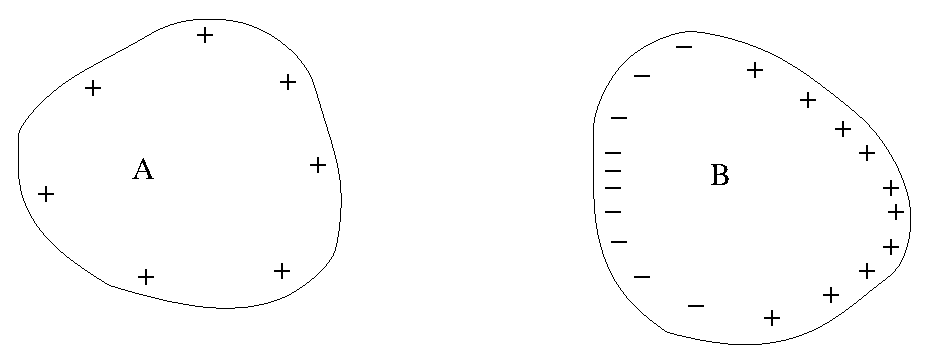
\includegraphics[scale=0.42]{immagini/fisica2/induz2}}
  \subfigure[$B$ modifica la distribuzione delle cariche su $A$]{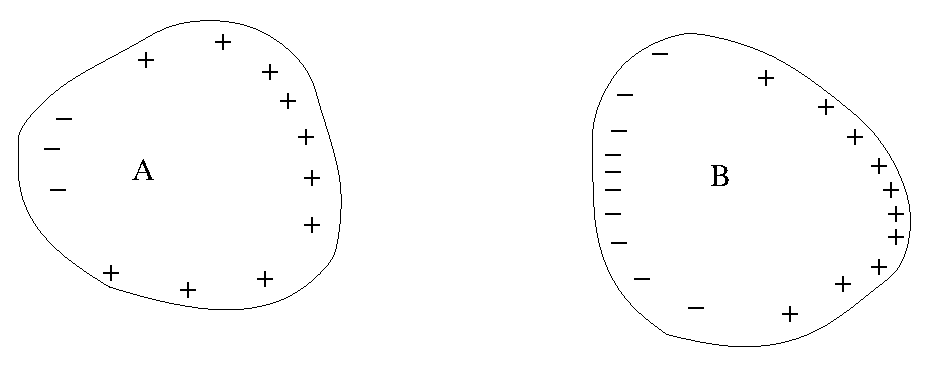
\includegraphics[scale=0.4]{immagini/fisica2/induz3}}
  \qquad
  \subfigure[$B$ è collegato a terra, formano un unico conduttore]{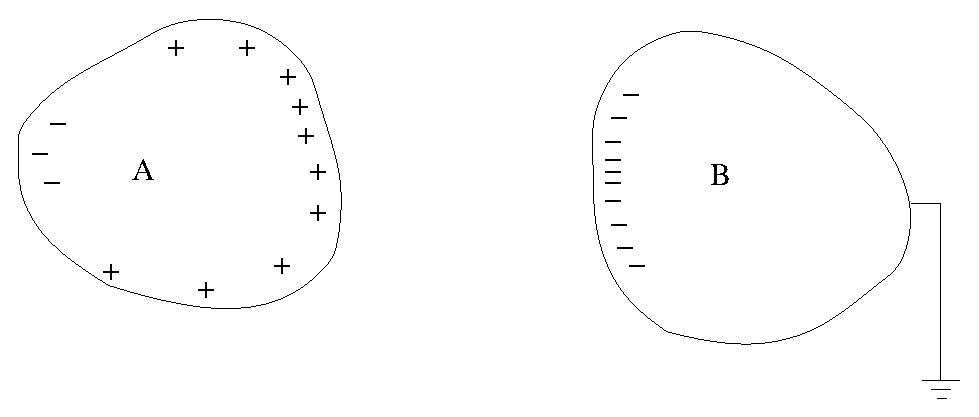
\includegraphics[scale=0.40]{immagini/fisica2/induz4}}\\
  \subfigure[$B$ da solo è carico]{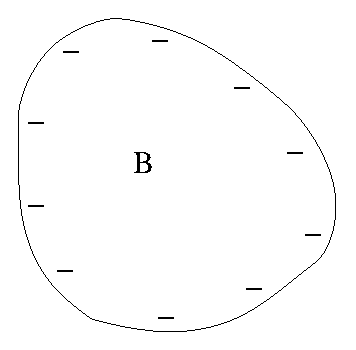
\includegraphics[scale=0.43]{immagini/fisica2/induz5}}
  \caption{Induzione elettrostatica.}
\end{figure}
\subsection{Induzione completa\index{induzione elettrostatica!completa}}
Consideriamo un conduttore cavo scarico. Poniamo all'interno del conduttore una carica $q$. Applichiamo il teorema di Gauss all'interno del conduttore. Il campo è zero, allora la carica totale interna al condensatore è nulla. Facendo tendere la superficie gaussiana alla superficie interna si scopre che ci deve essere una carica $-q$ sulla parete interna del conduttore che bilancia la carica $q$ interna, in modo che la carica totale interna alla superficie gaussiana sia nulla. Sulla superficie esterna invece ci deve essere una carica $q$ in modo che il corpo sia ancora complessivamente scarico. La carica indotta è uguale alla carica inducente. Questo fenomeno avviene solo quando il corpo inducente è totalmente racchiuso dal corpo indotto.
\begin{Es}[schermo elettrostatico\index{schermo elettrostatico} -- lo smerdatore]
  Im\-ma\-gi\-nia\-mo una fanciulla rinchiusa dentro un conduttore cavo. Adamo, all'esterno, ha molta voglia di sperimentare. Prova a farsi notare avvicinando una carica positiva al conduttore. Sull'esterno si accumula una carica negativa, all'interno positiva. La fanciulla non si accorge di niente essendo il campo elettrico interno invariato. La fanciulla, tutta sola, prova a farsi notare, agitando una carica positiva. Sulla parete interna si crea un accumulo di cariche positive, all'esterno negative, ma Adamo non percepisce nessuna variazione del campo elettrostatico. Il conduttore cavo funziona da schermo elettrostatico.
\end{Es}
\section{Potere dispersivo delle punte\index{potere dissipativo delle punte}}
In un conduttore carico la densità di carica sugli spigoli è maggiore che altrove. Consideriamo una punta carica nell'atmosfera vicino ad una candela. Si osserva che la fiamma oscilla a causa di un vento ionico. Infatti la carica sul conduttore attira ioni dell'atmosfera di segno opposto che lentamente neutralizzano la carica sul conduttore e contemporaneamente respinge gli ioni con lo stesso segno.. Si crea così un movimento di cariche, in questo caso particelle cariche dell'aria che muovono la fiamma. Per spiegare il fenomeno interpretiamo gli spigoli come zone dove il raggio di curvatura è più piccolo. Consideriamo allora due sfere cariche con raggi diversi $R>r$ collegate a grande distanza (niente induzione) da un filo. Sulla prima sfera:
\[V_1=\frac{1}{4\pi\varepsilon_0}\oint_{S_1}\frac{\sigma_R\ud a}{\norm{\ve r-\ve r\,'}}=\frac{1}{4\pi\varepsilon_0}\oint_{S_1}\frac{\sigma_R\ud a}{R}=\frac{1}{4\pi\varepsilon_0}\frac{\sigma_R}{R}4\pi R^2=\frac{\sigma_R R}{\varepsilon_0}=\frac{Q}{4\varepsilon_0\pi R}\]
Sulla seconda:
\[V_2=\frac{1}{4\pi\varepsilon_0}\oint_{S_2}\frac{\sigma_r\ud a}{\norm{\ve r-\ve r\,'}}=\frac{1}{4\pi\varepsilon_0}\oint_{S_2}\frac{\sigma_r\ud a}{r}=\frac{1}{4\pi\varepsilon_0}\frac{\sigma_r}{r}4\pi r^2=\frac{\sigma_r r}{\varepsilon_0}=\frac{q}{4\varepsilon_0\pi r}\]
ma $V_1=V_2$ perché un unico conduttore, allora:
\begin{equation}
  \frac{Q}{R}=\frac{q}{r}
  \label{candela01}
\end{equation}
La carica è proporzionale al raggio, la densità superficiale di carica:
\[\sigma_R=\frac{Q}{4\pi R^2}\qquad \sigma_r=\frac{q}{4\pi r^2}\]
Allora il rapporto tra le densità di carica (usando la precedente e la \eqref{candela01}):
\[\frac{\sigma_R}{\sigma_r}=\frac{Qr^2}{qR^2}=\frac{r}{R}<1\]
Dunque $\sigma_R<\sigma_r$ e, per il teorema di Coulomb, in prossimità dei conduttori:
\[E_r>E_R\]
\section{Capacità elettrica\index{capacità elettrica}}
Consideriamo un conduttore isolato. Carichiamolo con una carica $q$; il conduttore raggiungerà un certo pontenziale:
\[\varphi(\ve r)=\frac{1}{4\pi\varepsilon_0}\int_S\frac{\sigma(\ve r\,')\,\ud a'}{\norm{\ve r-\ve r\,'}}\]
Se aggiungiamo ancora $q$ arrivando a $2q$ anche il potenziale raddoppia. Si definisce:
\begin{Def}[capacità di un conduttore]
  \begin{equation}
    C=\frac{q}{V}
  \end{equation}
\end{Def}
Esso è costante, dipende solo dalla geometria del conduttore. Si misura in $\text{farad}=\si{\farad}=\frac{\text{coulomb}}{\text{volt}}$.
\begin{Es}[sfera]
  Calcoliamo la capacità di una sfera conduttrice di raggio $R$. Sapendo che la carica si distribuisce uniformemente per simmetria:
  \[\sigma(\ve r)=\frac{Q}{4\pi R^2}=\sigma\]
  \[\varphi(\ve r)=\frac{1}{4\pi\varepsilon_0}\oint_S\frac{\sigma(\ve r\,')\,\ud a'}{R}=\frac{1}{4\pi\varepsilon_0}\frac{Q}{4\pi R^2 R}4\pi R^2=\frac{1}{4\pi\varepsilon_0}\frac{Q}{R}\]
  \[C=\frac{Q}{\varphi}=4\pi\varepsilon_0R\]
  Se $R=\SI{1}{\metre}$ allora $C=\SI{1E-10}{\farad}$. Il farad è un'unità generalmente grande.
\end{Es}
\subsection{Condensatore}
Mettere troppa carica su un conduttore è difficile perché questa tende a dissiparsi nell'aria. \`E invece più pratico aumentare la capacità

Usiamo due conduttori, sia $A$ carico e quindi con un certo potenziale $V_0$ e $B$ scarico. $A$ induce delle cariche su $B$ e $B$ modifica la distribuzione delle cariche di $A$. Ora il potenziale di $A$ $V_A$ è minore del potenziale iniziale, a causa delle cariche di segno opposto sul lato di $B$ rivolto verso $A$. Quindi $V_A<V_0$ e allora se all'inizio $C=\frac{Q}{V_0}$ e ora $C'=\frac{Q}{V_A}$ e la carica $Q$ è costante si ha che $C'>C$. Abbiamo aumentato la capacità del condensatore.
\begin{Def}[condensatore]
  Il condensatore è un sistema formato da due conduttori adiacenti, isolati, carichi, con cariche di uguale valore, ma di segno opposto e tali da subire la stessa influenza elettrostatica da parte di altri conduttori.
\end{Def}
\begin{figure}[htbp]
  \centering
  \includegraphics[scale=1.5]{immagini/fisica2/cond1}
  \caption{simbolo del condensatore.}
\end{figure}
Se colleghiamo il corpo $B$ a terra otteniamo un condensatore. I due conduttori sono chiamati piatti o armature del condensatore.
\begin{Def}[carica del condensatore]
  La carica del condensatore è il valore assoluto della carica immagazzinata da uno dei due conduttori di un condensatore.
\end{Def}
\begin{Def}[capacità del condensatore]
  \[C=\frac{Q}{\Delta V}\]
  con $Q$ la carica del condensatore e $\Delta V$ la differenza di potenziale tra le due armature.
\end{Def}
Essa dipende solo dalla geometria del condensatore.
\subsubsection{Esempi di geometrie}
\begin{Es}[piano]
  Consideriamo due lastre infinite $A$ e $B$ parallele, a distanza $d$. La carica si distribuisce uniformemente:
  \[\sigma=\frac{Q}{S}\]
  Il campo del condensatore è
  \[\ve E=\frac{\sigma}{\varepsilon_0}\ver \imath\]
  \[\Delta V=V_B-V_A=-\int_A^B\ve E\cdot\ud l=-\ve E\int_A^B\ud l=-\frac{\sigma}{\varepsilon_0}d\]
  \[C=\frac{Q}{\Delta V}=\frac{\sigma S}{\sigma d}\varepsilon_0=\frac{S}{d}\varepsilon_0\]
  Da questo esempio si deduce che $\varepsilon_0$ si può esprimere in \si{\farad\per\meter}.
\end{Es}
\begin{Es}[sferico]
  Consideriamo due sfere con raggi $a<b$ concentriche. Sia $q$ la carica del condensatore. Il campo all'interno può essere calcolato con Gauss. Pensiamo una superficie gaussiana sferica con raggio $r:a<r<b$ concentrica al condensatore. Allora:
  \[\Phi_S(\ve E)=E 4\pi r^2=\frac{Q}{\varepsilon_0}=\frac{q}{\varepsilon_0}\qquad \ve E=\frac{1}{4\pi\varepsilon_0}\frac{q}{r^2}\ver e_r\]
  diretto radialmente, il verso è dato dal segno di $q$. Calcoliamo la differenza di potenziale tra le due sfere scegliendo un percorso $\Gamma$ radiale:
  \[\Delta V=\int_\Gamma\ve E\cdot\ud\ve s=\int_\Gamma E\ud r=\frac{q}{4\pi\varepsilon_0}\int_a^b\frac{1}{r^2}\ud r=\frac{q}{4\pi\varepsilon_0}\left(\frac{1}{a}-\frac{1}{b}\right)\]
  \[C=\frac{q}{\Delta V}=\frac{q4\pi\varepsilon_0}{q}\left(\frac{ab}{b-a}\right)=4\pi\varepsilon_0\frac{ab}{b-a}\]
\end{Es}
\begin{Es}[cilindrico]
  Consideriamo un condensatore formato da due cilindri coassiali con raggi $a<b$ e altezza $h$. Sia $q$ la carica del condensatore. Per calcolare il campo serviamoci di una superficie gaussiana cilindrica coassiale di altezza $h$ con raggio $r:a<r<b$, consideriamo il condensatore infinito:
  \[\Phi_S(\ve E)=E2\pi rh=\frac{Q}{\varepsilon_0}=\frac{q}{\varepsilon_0}\qquad \ve E=\frac{1}{2\pi\varepsilon_0}\frac{q}{hr}\ver e_r\]
  diretto perpendicolarmente ai due cilindri. La differenza di potenziale tra le due armature è
  \[\Delta V=\int_\Gamma\ve E\cdot\ud\ve s=\int_\Gamma E\ud r=\frac{q}{2\pi\varepsilon_0h}\int_a^b\frac{\ud r}{r}=\frac{q}{2\pi\varepsilon_0h}\log\frac{b}{a}\]
  \[C=\frac{q}{\Delta V}=\frac{2\pi\varepsilon_0h}{\log\frac{b}{a}}\]
\end{Es}
\subsection{Energia di un condensatore}
Tra le altre cose un condensatore serve per immagazzinare energia\footnote{per esempio nei flash delle macchine fotografiche}. Sappiamo che l'energia potenziale di un sistema di cariche è
\[W=\frac{1}{2}\sum q_i\varphi_i\]
$\varphi_i$ è il potenziale delle cariche nelle loro posizioni. \`E anche il lavoro necessario per portare le cariche dall'infinito alla loro posizione. Se lavoriamo con distribuzioni di cariche allora:
\[W=\frac{1}{2}\int_S\Bigl(\sigma(x,y,z)\ud a\varphi(x,y,z)\Bigr)+\frac{1}{2}\int_V\Bigl(\rho(x,y,z)\ud v\varphi(x,y,z)\Bigr)\]
Stiamo parlando di conduttori e quindi la carica si distribuisce sulla superficie. Siano $S_1,\ldots,S_n$ le superfici:
\[W=\frac{1}{2}\sum_{i=1}^N\int_{S_i}\varphi_{S_i}\sigma_i\,\ud a_i=\frac{1}{2}\sum_{i=1}^N\varphi_{S_i}q_{i}\]
Nel caso del condensatore $N=2$, $q_1=-q_2=q$:
\[W=\frac{1}{2}\left(|q|\varphi_A-|q|\varphi_B\right)=\frac{1}{2}|q|\Delta V\]

\begin{Es}[condensatore piano]
  Calcoliamo l'energia di un condensatore piano in un altro modo. L'energia può essere intesa come il lavoro necessario per carica le due armature portando le cariche dall'armatura $B$ all'armatura $A$. Siano inizialmente scarichi. Se porto $\ud q$ da $B$ a $A$ non compio lavoro, perché non c'è campo elettrico che mi ostacola. Per portare la seconda carica $\ud q$ devo compiere un lavoro:
  \[\ud W=\ud q\Delta V\]
  Integrando:
  \[W=\int_0^Q\ud W=\int_0^Q\ud q\Delta V=\int_0^Q\frac{q}{C}\,\ud q=\frac{Q^2}{2C}=\frac{1}{2}Q\Delta V\]
\end{Es}

Usando la definizione di capacità l'energia può essere scritta in modi diversi:
\begin{equation}
  W=\frac{1}{2}C\Delta V^2=\frac{1}{2}Q\Delta V=\frac{1}{2}\frac{Q^2}{C}
\end{equation}
L'energia è sotto forma di campo elettrostatico.


\begin{Es}[Lavoro per spostare una armatura]
  Sia un condensatore a facce piane e parallele di superficie $S$, con carica $Q$ a distanza $d_0$. Considerando il caso a carica e potenziale costante (isolato o collegato ad un generatore) vogliamo conoscere il lavoro per spostare le armature a distanza $d_F$, la variazione di energia e il potenziale finale.

  Consideriamo il caso isolato. $Q=\const$.
  \begin{equation*}
    \begin{aligned}
      \text{inizio} & \qquad & C_0=\varepsilon_0\dfrac{S}{d_0} & W_0 = \frac{1}{2}\frac{Q^2}{C_0}
      \\
      \text{fine}   & \qquad & C_F=\varepsilon_0\dfrac{S}{d_F} & W_F = \frac{1}{2}\frac{Q^2}{C_F}
    \end{aligned}
  \end{equation*}
  Il lavoro lo possiamo calcolare come variazione di energia potenziale $L_C=-\Delta W$; ma noi vogliamo il lavoro fatto contro le forze del campo: $L=-L_C$:
  \[
    L=W_F-W_0=\frac{1}{2}Q^2\left(\frac{1}{C_F}-\frac{1}{C_0}\right) = \frac{1}{2}\frac{Q^2}{\varepsilon_0 S}\left(d_F-d_0\right)
  \]
  Oppure lo possiamo calcolare dalla forza:
  \[\delta L=\ve F\cdot\ud \ve x=QE\ud x=Q\frac{\sigma}{2\varepsilon_0}\ud x=Q\frac{Q}{2S\varepsilon_0}\ud x=\frac{1}{2}\frac{Q^2}{\varepsilon_0 S}\ud x\]
  La forza la si poteva anche ricavare da $\delta F=\ud W$. La forza risulta costante, grazie al fatto che nell'approssimazione il campo campo è costante e parallela allo spostamento.
  \[L=\int_{d_0}^{d_F}\delta L=\frac{1}{2}\frac{Q^2}{\varepsilon_0 S}(d_F-d_0)\]
  La variazione di energia potenziale del sistema è uguale al lavoro fatto dall'esterno.

  Consideriamo ora il caso di potenziale $\Delta V=\const$.
  \[\delta L=\ve F\cdot\ud \ve x=QE\ud x=\frac{Q^2}{2\varepsilon_0S}\ud x=\frac{C^2\Delta V^2}{2\varepsilon_0S}\ud x=\frac{\varepsilon_0^2S^2\Delta V^2}{2\varepsilon_0Sx^2}\ud x=\frac{\varepsilon_0S\Delta V^2}{2x^2}\ud x\]
  \[L=\int_{d_0}^{d_F}\delta L=\frac{\varepsilon_0S\Delta V^2}{2}\int_{d_0}^{d_F}\frac{1}{x^2}\ud x=\frac{1}{2}\varepsilon_0\left(\frac{1}{d_0}-\frac{1}{d_F}\right)\Delta V^2S\]
  Non possiamo più dire che la variazione di energia potenziale è il lavoro, perché il condensatore non è isolato, anche il generatore compie lavoro.
  \begin{align*}
    \Delta W & =W_F-W_0=\frac{1}{2}C_F\Delta V^2-\frac{1}{2}C_0\Delta V^2=\frac{1}{2}V^2\left(\varepsilon_0\frac{S}{d_F}-\varepsilon_0\frac{S}{d_0}\right) \\
             & =\frac{1}{2}\varepsilon_0\left(\frac{1}{d_F}-\frac{1}{d_0}\right)\Delta V^2S
  \end{align*}
\end{Es}
\subsection{Condensatori in serie e in parallelo}
\subsubsection{Serie}
\begin{figure}[htbp]
  \centering
  \includegraphics[scale=1.2]{immagini/fisica2/cond2}
\end{figure}
$n$ condensatori sono collegati in serie quando la $\Delta V$ ai capi della combinazione è la somma delle $\Delta V_i$. Siano all'inizio scarichi. Se poniamo una carica $q$ sull'armatura del primo condensatore allora sulla seconda armatura del primo condensatore si crea per induzione una carica opposta $-q$ e sulla prima armatura del secondo condensatore una carica $q$ in modo che la somma della seconda armatura del primo condensatore e la prima del secondo condensatore, che formano un unico conduttore, sia nulla. Se poi l'ultimo condensatore lo colleghiamo a terra avremo che per ogni condensatore si avrà una carica $q$ sulla prima armatura e $-q$ sulla seconda. La carica di ogni condensatore è allora la stessa, quindi la differenza di potenziale di ogni condensatore dipenderà solo dalla propria capacità
\[\Delta\varphi_i=\frac{q}{C_i}\]
Abbiamo detto che la differenza di potenziale tra i capi $A$ e $B$ è la somma delle differenze di potenziali:
\[\varphi_A-\varphi_B=\sum_{i=1}^N\varphi_i=\sum_{i=1}^N\frac{q}{C_i}=q\sum_{i=1}^N\frac{1}{C_i}\]
Il condensatore equivalente, cioè quello che sostituito al sistema in serie produce gli stessi effetti, è quello con capacità
\[\frac{1}{C_\text{eq}}=\sum_{i=1}^N\frac{1}{C_i}\]
\subsubsection{Parallelo}
\begin{figure}[htbp]
  \centering
  \includegraphics[scale=0.5]{immagini/fisica2/cond3}
\end{figure}
In parallelo la differenza di potenziale di ogni condensatore è uguale. La somma delle cariche è
\[Q=\sum_{i=1}^N q_i=\sum_{i=1}^N C_i\varphi\]
Allora il condensatore equivalente ha capacità
\[C_\text{eq}=\sum_{i=1}^N C_i\]

\chapter{Problema generale dell'elettrostatica}
\minitoc
Abbiamo detto che l'elettrostatica è descritta completamente solo da due leggi:
\begin{subequations}



  \begin{gather}
    \ve\nabla\cdot\ve E=\frac{\rho}{\varepsilon_0}
    \label{eq:div_E}\\
    \ve\nabla\times\ve E=0
    \label{eq:rot_E}
  \end{gather}
\end{subequations}
Dalla \eqref{eq:rot_E} che ci dice che $\ve E$ è irrotazionale, sappiamo che deve esistere una funzione scalare che è il potenziale di $\ve E$:
\begin{equation}
  \ve E=-\ve\nabla\varphi
  \label{eq:poisson_pot}
\end{equation}
Sostituendola nella \eqref{eq:div_E}, che non abbiamo ancora usato, otteniamo una singola equazione:
\begin{equation}
  \nabla^2\varphi=-\frac{\rho}{\varepsilon_0}
  \label{eq:Poisson01}
\end{equation}
Si può anche scrivere:
\[\nabla^2\varphi=\ve\nabla\cdot\ve\nabla\varphi=\diver\grad\varphi={\frac{\partial^2 \varphi}{\partial x^2}+\frac{\partial^2 \varphi}{\partial y^2}+\frac{\partial^2 \varphi}{\partial z^2}}=-\frac{\rho}{\varepsilon_0}\]
L'operatore $\nabla^2$ è il laplaciano\index{laplaciano} e l'equazione differenziale alle derivate parziali \eqref{eq:Poisson01} è l'equazione di Poisson\index{equazione!di Poisson}\index{Poisson}. Risolvere l'equazione di Poisson significa trovare $\varphi(\ve r)$ in funzioni delle condizioni del problema. Dalla conoscenza di $\varphi$: $\ve E=-\ve\nabla\varphi$. L'elettrostatica può essere quindi descritta, oltre che dalle equazioni~\eqref{eq:div_E} e \eqref{eq:rot_E}, dalle equazioni \eqref{eq:Poisson01} e \eqref{eq:poisson_pot}. Il problema così forumulato è ora più semplice, in quanto l'equazione \eqref{eq:poisson_pot} è semplicemente il calcolo di un gradiente, mentre l'equazione \eqref{eq:Poisson01} pur essendo di un ordine superiore all'originale, riguarda una funzione scalare e può essere facilmente generalizzato, per esempio se la sorgente del campo è data esclusivamente da cariche elettriche in un volume allora l'unica soluzione è
\[\varphi(\ve r)=\frac{1}{4\pi\varepsilon_0}\int_V\frac{\rho(\ve r\,')}{\norm{\ve r-\ve r\,'}}\,\ud v'\]
Il problema diventa più complesso quando si inseriscono dei conduttori che subiscono l'induzione elettrostatica.
\section{Funzioni armoniche}
In assenza di carice, cioè $\rho=0$, l'equazione di Poisson si riduce a:
\begin{equation}
  \nabla^2\varphi=0
  \label{eq_laplace}
\end{equation}
conosciuta come equazione di Laplace\index{equazione!di Laplace}\index{Laplace}.
\begin{Def}[Funzione armonica] Una funzione che soddisfa la \eqref{eq_laplace} e che abbia derivate prime continue è detta armonica\index{funzione!armonica}.
\end{Def}
Quindi in assenza di cariche $\varphi$ è armonica. La zona di armonicità di una funzione è l'insieme dei punti dove la funzione è armonica.
\subsection{Teoremi}
I problemi di elettrostatica vengono formulati attraverso le condizioni di Dirichlet o di Neumann. Le prime impogono che la funzione $\varphi$ assuma determinati valori su una superficie, le seconde invece impongono condizioni sulle derivate normali (derivata direzionale rispetto alla normale della superficie).
\begin{Teo}[unicità  problema di Dirichlet]
  Data una superficie chiusa $S$ la funzione armonica che su $S$ assume il valore $\varphi_S$ è unica.
\end{Teo}
$\varphi_S$ non deve essere necessariamente una costante.
\begin{Teo}[unicità  problema di Neumann]
  Siano $\varphi_1$ e $\varphi_2$ due funzioni armoniche definite in un volume tali che le derivate normali siano uguali, allora $\varphi_1$ e $\varphi_2$ differiscono per una costante.
\end{Teo}
\begin{Teo}[media]
  Sia $S$ una sfera contenuta in una zona di armonicità di $\varphi$. Allora il valor medio che $\varphi$ assume sulla superficie di $S$ è uguale al valore che $\varphi$ assume nel centro della sfera.
  \begin{equation}
    \varphi(\ve r)=\frac{1}{4\pi R^2}\int_S\varphi(\ve r\,')\,\ud a'
  \end{equation}
\end{Teo}

Come conseguenza $\varphi$ non ha minimi o massimi locali (oppure se $\varphi$ ha un minimo o un massimo locale allora è costante). Infatti se $\varphi$ avesse un minimo locale allora il valore in quel punto sarebbe minore della media e quindi la media sarebbe minore del valore in quel punto. I valori estremi di $\varphi$ sono sul bordo del dominio.
\begin{Teo}[Earnshaw]
  Non esistono soluzioni stazionarie dell'equazione di Laplace che abbiano un minimo locale. Questo significa che una carica elettrica non può essere in equilibrio stabile in un campo esclusivamente elettrostatico.
\end{Teo}

\section{Soluzione dell'equazione di Laplace}
Tentiamo di risolvere l'equazione di Laplace, cioè quando non ci sono cariche libere, in casi particolari.
\subsection{Soluzione generale}
\subsubsection{Coordinate cartesiane}
\begin{multline}
  \varphi(x,y,z)=\left(A\sin k_x x+B\cos k_x x\right)\left(C\sin k_y y+D\cos k_y y\right)\\\left(Ee^{\sqrt{-k_z^2+k_y^2}z}+Fe^{\sqrt{k_z^2+K_y^2}z}\right)
\end{multline}
\subsubsection{Coordinate cilindriche}
\begin{equation}
  \varphi(r,\theta,z)=\left(A\log r+B\right)\left(C\theta+D\right)\left(Ez+F\right)
\end{equation}
\subsubsection{Coordinate sferiche}
\begin{equation}
  \varphi(r,\theta,\phi)=\sum_{l,m}\left(E_lr^l+F_lr^{-(l+1)}\right)\left(C_lP_l^m+D_lQ_l^m\right)\left(A\sin m\phi+B\cos m\phi\right)
\end{equation}
\section{Caso monodimensionale}
Supponiamo che il potenziale $\varphi$ dipenda solo dalla coordinata $x$, allora $\frac{\partial\varphi}{\partial y}=\frac{\partial\varphi}{\partial z}=0$ e l'equazione di Laplace diventa:
\[\frac{\ud^2\varphi}{\ud x^2}=0\]
Allora:
\[\frac{\ud \varphi}{\ud x}=a\qquad \varphi=ax+b\]
\begin{Es}[condensatore]
  Consideriamo due piani paralleli, tenuti a potenziali $\varphi_1<\varphi_2$, a distanza $d$. Possiamo usare l'equazione di Laplace perché non ci sono cariche libere. Vogliamo il potenziale tra i due piani. Esso dipende solo dalla coordinata $x$ e quindi è un problema monodimensionale. Sia primo piano di equazione $x=0$. La soluzione generale è
  \[\varphi(x)=ax+b\]
  Le condizioni al contorno sono:
  \[\varphi(0)=\varphi_1\qquad\varphi(d)=\varphi_2\]
  Allora:
  \[\varphi(x)=\frac{\varphi_2-\varphi_1}{d}x+\varphi_2\]
  Il campo:
  \[\ve E_E=-\ve\nabla\varphi=\frac{\varphi_1-\varphi_2}{d}\ver \imath\]
  Usando il teorema di Coulomb \eqref{eq:teo_coulomb}:
  \[\sigma=\varepsilon_0E=\frac{\varphi_1-\varphi_2}{d}\varepsilon_0\]
\end{Es}
\begin{Es}[sfera in condensatore]
  Sia una sfera conduttrice di raggio $R$ al centro di un condensatore a facce piane e parallele. Consideriamo un sistema di riferimento centrato nella sfera. Sia $\pm\sigma$ la densità di carica sulle facce a distanza $2d$, allora il campo elettrico esterno, cioè prodotto dal condensatore è
  \[\ve E=\frac{\sigma}{\varepsilon_0}\ver \imath\]
  fissiamo il riferimento del potenziale sulla prima armatura che poniamo a terra. Il potenziale esterno:
  \[\varphi_{E}(x)=-\frac{\sigma}{\varepsilon_0}(x+d)\]
  Usiamo le coordinate polari. Sia $\ve R$ tale che $\norm{\ve R}=R$. Il potenziale esterno sulla superficie del conduttore:
  \[\varphi_E(\ve R)=-\frac{\sigma}{\varepsilon_0}\left(R\cos\theta+d\right)\]
  Le cariche indotte sulla sfera produrranno un campo e un potenziale indotto che si sommerà
  \[\varphi_T=\varphi_E+\varphi_I\]
  Il conduttore è una superficie equipotenziale e quindi $\varphi_T$ deve essere costante.
  \[\varphi_T(\ve R)=\varphi_E(\ve R)+\varphi_I(\ve R)=\const\]
  \begin{align*}
    \varphi_I(\ve R) & =\const-\varphi_E(\ve R)=\const+\frac{\sigma}{\varepsilon_0}(R\cos\theta+d)=\const+\frac{\sigma}{\varepsilon_0}d+\frac{\sigma}{\varepsilon_0}R\cos\theta \\
                     & =\const+\frac{\sigma}{\varepsilon_0}d+\frac{\sigma}{\varepsilon_0}\ve R\cdot\ver \imath
  \end{align*}
  e mho?
\end{Es}

\section{Metodo delle cariche immagine}
Il metodo delle cariche immagine è talvolta utile in problemi al bordo, cioè con superfici di tenute ad un potenziale fisso e conosciuto, nei quali siano presenti anche cariche libere. A volte è possibile simulare l'effetto delle superfici con delle cariche opportune posizionate all'esterno del volume di interesse, chiamate cariche immagine.
\begin{Es}[carica e piano infinito]
  \label{es:carica_e_piano_infinito}
  Sia una carica $q$ posizionata sull'asse $x_+$ e sia il piano $y-z$ tenuto a terra. La stessa situazione si realizza con la carica $q$ e una carica immagine $-q$ posizionata simmetricamente rispetto alla carica reale. Infatti il potenziale delle due cariche:
  \[
    \varphi(x,y,z)=\frac{1}{\giorgi}\left(\frac{q}{\sqrt{(x-x_+)^2+y^2+z^2}}+\frac{-q}{\sqrt{(x-x_-)^2+y^2+z^2}}\right)
  \]
  e sul piano ($x=0$):
  \[
    \varphi(0,y,z)=\frac{1}{\giorgi}\left(\frac{q}{\sqrt{x_+^2+y^2+z^2}}+\frac{-q}{\sqrt{x_-^2+y^2+z^2}}\right)=0
  \]
  in quanto $x_+ = -x_-$. La somma del potenziali delle due cariche è la soluzione per il semispazio di destra ($x>0$). Nel semispazio in cui c'è la carica di prova invece il potenziale è costante, e in questo caso nullo, in quanto il semispazio di sinistra si può considerare come uno spazio interno al conduttore piano infinito. Per determinare la densità di carica sul piano serve la componente normale del campo elettrostatico:
  \[
    E_x(0,y,z) = -\frac{\partial\varphi}{\partial x}(0,y,z) = -\frac{q}{2\pi\varepsilon_0}\frac{x_+}{(x_+^2+y^2+z^2)^{3/2}}
  \]
  quindi usando il teorema di Coulomb \eqref{eq:teo_coulomb}:
  \[
    \sigma = \varepsilon_0 E_x = -\frac{qd}{2\pi(d^2+y^2+z^2)^{3/2}}
  \]
  Integrando su tutto il piano si ottiene:
  \begin{equation*}
    \begin{aligned}
      Q & = \int_\text{piano} \sigma\,\ud a = \int -\frac{qd}{2\pi(d^2+y^2+z^2)^{3/2}}\,\ud y\,\ud z \\
        & = -\int \frac{qd}{2\pi(d^2+\rho^2)^{3/2}} \rho\,\ud\rho\sin\theta\,\ud\theta               \\
        & = -\frac{2\pi qd}{2\pi}\int_0^\infty \frac{\rho\ud\rho}{(d^2+\rho^2)^{3/2}}                \\
        & = -qd\int_{d^2}^\infty \frac{\ud t}{2t^{3/2}} = -q
    \end{aligned}
  \end{equation*}
  avendo usato la sostituzione $t=\rho^2+d^2$ e il fatto che l'integrando non dipende da $\theta$. Il risultato significa che la carica indotta sulla superficie del conduttore piano è uguale ed opposta alla carica reale, infatti si tratta di induzione completa.
\end{Es}
\begin{Es}[carica e sfera]
  Consideriamo una sfera centrata nell'origine di raggio $a$ a potenziale nullo. Consideriamo una carica puntiforme $q$ a distanza $d$ dall'origine. Supponendo che sia sufficiente una sola carica immagine sicuramente la sua posizione per simmetria sarà sulla congiungente del centro della sfera e la carica reale. In generale il potenziale generato dalle due cariche:
  \begin{equation*}
    \begin{aligned}
      \varphi(\ve x) & = \frac{1}{\giorgi}\left(\frac{q}{\norm{\ve x -\ve d}}+\frac{q'}{\norm{\ve x-\ve d'}}\right)           \\
                     & = \frac{1}{\giorgi}\left(\frac{q}{\norm{x\ver n -d\ver n'}}+\frac{q'}{\norm{x\ver n-d'\ver n'}}\right)
    \end{aligned}
  \end{equation*}
  dove $\ver n$ è il versore di $\ve x$ e $\ver n'$ è il versore di $\ve d$ e anche di $\ve d'$. Sulla sfera:
  \begin{equation*}
    \begin{aligned}
      \varphi(x=a) & = \frac{1}{\giorgi}\left(\frac{q}{\norm{a\ver n -d\ver n'}}+\frac{q'}{\norm{a\ver n-d'\ver n'}}\right)                       \\
                   & = \frac{1}{\giorgi}\left(\frac{q}{a\norm{\ver n -\frac{d}{a}\ver n'}}+\frac{q'}{a\norm{\ver n-\frac{d'}{a}\ver n'}}\right)=0
    \end{aligned}
  \end{equation*}
  quindi una soluzione è $d=d'$ e $q=-q'$ ma non va bene, perché $q'$ è all'esterno della sfera. Quindi raccogliendo in modo diverso:
  \begin{equation*}
    \begin{aligned}
      \varphi(x=a) & = \frac{1}{\giorgi}\left(\frac{q}{a\norm{\ver n-\frac{d}{a}\ver n'}}+\frac{q'}{d'\norm{\ver n'-\frac{a}{d'}\ver n}}\right)                                                                        \\
                   & = \frac{1}{\giorgi}\left(\frac{q}{a\left(1+\frac{d^2}{a^2}-2\frac{d}{a}\ver n\cdot\ver n'\right)^{1/2}}+\frac{q'}{d'\left(1+\frac{a^2}{d'^2}-2\frac{a}{d'}\ver n\cdot\ver n'\right)^{1/2}}\right)
    \end{aligned}
  \end{equation*}
  e deve essere:
  \[
    \frac{q}{a}=-\frac{q'}{d'}\qquad \frac{d}{a}=\frac{a}{d'}
  \]
  in modo che il potenziale si annulli sulla sfera per ogni possibile valore di $\ver n\cdot\ver n'$.  Quindi per la carica immagine:
  \[
    q'=\frac{-a}{d}q\qquad d'=\frac{a^2}{d}
  \]
  In questo caso la carica immagine è all'interno della sfera, in quando $a < d\Rightarrow d'<a$. Quindi il potenziale:
  \[
    \varphi(\ve x) = \frac{1}{\giorgi}\left(\frac{q}{\norm{x\ver n -d\ver n'}}+\frac{-\frac{a}{d}q}{\norm{x\ver n-\frac{a^2}{d}\ver n'}}\right)
  \]
  \begin{figure}[htbp]
    \centering
    \includegraphics{immagini/fisica2/sfera_neutra}
    \caption{Linee equipotenziali e linee di campo nel piano $y=0$. Le linee rosse indicano le regioni dove non è stato calcolato il potenziale. La sfera ha raggio $2$, mentre la carica unitaria positiva è in $(0,8)$. Il punto indica la posizione della carica immagine.}
  \end{figure}
\end{Es}

\begin{Es}[sfera in campo uniforme]
  \begin{figure}[htbp]
    \centering
    \begin{tikzpicture}[scale=1]
\coordinate (O) at (0,0);
\coordinate (q) at (0.5,0);
\coordinate (-q) at (-0.5,0);
\coordinate (p) at (xyz polar cs:angle=25, radius=3.5);
\draw[->] (-6,0) -- (6,0) node[above] {$z$};
\draw[->] (0,-2) -- (0,2);
\draw (O) circle (1.5cm);
\draw[<->] (O) -- (xyz polar cs:angle=250, radius=1.5) node[near end,sloped,above]{$a$};
\filldraw[black] (4.5,0) circle(2pt) node[below right]{$-Q$};
\draw[->,shorten >=2pt] (O) -- (4.5,0) node[near end,above]{$\ve R_-$};
\filldraw[black] (-4.5,0) circle(2pt) node[below left]{$+Q$};
\draw[->,shorten >=2pt] (O) -- (-4.5,0) node[near end,above]{$\ve R_+$};
\filldraw[black] (-q) circle(2pt) node[below left]{$-q$};
\filldraw[black] (q) circle(2pt) node[below right]{$+q$};
\draw (2,0) arc (0:25:2.0cm) node[below right]{$\theta$};
\draw[->,shorten >=2pt] (O) -- (p) node[midway, above]{$\ve r$};
\filldraw[black] (p) circle(2pt) node[above
  right]{$P$};
\draw[dotted] (-q) -- (-0.5,0.8);
\draw[<->] (-0.5,0.8) -- (0,0.8) node[midway,above]{$d'$};
\end{tikzpicture}%

    \caption{La sfera a potenziale nullo può essere sostituita da due cariche immagine al suo interno.}
    \label{fig:esempio_campo_sfera}
  \end{figure}

  Consideriamo un campo uniforme di modulo $E_0$ diretto come l'asse $z$ e una sfera conduttrice centrata nell'origine, di raggio $a$ messa a terra. Il campo uniforme può essere simulato da due cariche puntiformi poste all'infinito in direzioni opposte di carica opposta (vedi fig.~\ref{fig:esempio_campo_sfera}). Infatti il potenziale:
  \[
    \begin{aligned}
      \varphi(\ve r)= & \frac{1}{\giorgi}\frac{Q}{\norm{\ve r - \ve R_+}}+\frac{1}{\giorgi}\frac{-Q}{\norm{\ve r-\ve R_-}}                                                               \\
      =               & \frac{Q}{\giorgi}\left\{\frac{1}{(r^2+R^2_+-2\ve r\cdot \ve R_+)^{1/2}}-\frac{1}{(r^2+R_-^2-2\ve r\cdot\ve R_-)^{1/2}}\right\}                                   \\
      =               & \frac{Q}{\giorgi}\frac{1}{R}\left\{\frac{1}{(\frac{r^2}{R^2}+1+2\frac{r}{R}\cos\theta)^{1/2}}-\frac{1}{(\frac{r^2}{R^2}+1-2\frac{r}{R}\cos\theta)^{1/2}}\right\}
    \end{aligned}
  \]
  si noti che l'angolo tra $\ve R_-$ e $\ve r$ è $\theta$, mentre l'angolo tra $\ve R_+$ e $\ve r$ è $\pi-\theta$. Usando il solito sviluppo usanto anche per lo sviluppo in multipoli:
  \[
    \begin{aligned}
      \left(1+\frac{r^2}{R^2}\pm\frac{2r}{R}\cos\theta\right)^{-1/2} & =1-\frac{1}{2}\left(\frac{r^2}{R^2}\pm\frac{2r}{R}\cos\theta\right)+o\left(\frac{r^2}{R^2}\pm\frac{2r}{R}\cos\theta\right) \\
                                                                     & =1\mp\frac{r}{R}\cos\theta+o\left(\frac{r}{R}\right)
    \end{aligned}
  \]
  quindi l'approssimazione per $R\to\infty$:
  \[
    \varphi(\ve r)=-\frac{1}{\giorgi}\frac{2Q}{R^2}\underbrace{r\cos\theta}_z=-\frac{1}{\giorgi}\frac{2Q}{R^2}z
  \]
  sempre che il rapporto $\frac{Q}{R^2}$ rimanga finito. Il campo elettrico è nullo in tutte le componenti tranne:
  \[
    E_z = \frac{1}{\giorgi}\frac{2Q}{R^2}
  \]
  poiché $E_z=E_0$ si ricava che $\frac{2Q}{R^2} = \giorgi E_0$.

  Ora bisogna aggiungere delle cariche immagine in modo tale che sulla supreficie della sfera il potenziale risulti nullo. Le due cariche dovranno essere all'interno della sfera. Per simmetria dovranno essere sull'asse $z$, poste in maniera simmetrica. Si può usare l'esempio precedente per ricavare il loro valore e la loro posizione. Consideriamo, grazie al principio di sovrapposizione separatamente la carica $Q$ e la carica $-Q$. Se abbiamo solo la carica $Q$ ci servirà una carica immagine di valore $-\frac{a}{R}Q$ e posta a $d'=\frac{a^2}{R}$ (vedi esercizio precedente). Discorso analogo per la carica $-Q$. Quindi il potenziale generato dalle quattro cariche risulta:
  \[
    \begin{aligned}
      \varphi(\ve r)=\frac{Q}{\giorgi}\Biggl\{\frac{1}{(r^2+R^2+2rR\cos\theta)^{1/2}}-\frac{1}{(r^2+R-2rR\cos\theta)^{1/2}}- \\
      -\frac{\frac{a}{R}}{(r^2+d'^2+2d' r\cos\theta)^{1/2}}+\frac{\frac{a}{R}}{(r^2+d'^2-2d' r\cos\theta)^{1/2}}\Biggr\}
    \end{aligned}
  \]
  i primi due termini sono quelli di prima. Ora per fare $R\to\infty$ gli ultimi due termini si espandono in maniera analoga:
  \[
    \left(r^2+\frac{a^4}{R^2}\pm 2\frac{a^2}{R}r\cos\theta\right)^{-1/2} = r^{-1}\left(1\mp\frac{a^2}{Rr}\cos\theta+o\left(\frac{a^2}{Rr}\right)\right)
  \]
  mettendo tutto insieme:
  \[
    \varphi(\ve r) = \frac{Q}{\giorgi}\left\{\frac{2}{R^2}r\cos\theta+\frac{2a^3}{R^2r^2}\cos\theta\right\}
  \]
  si noti che la coppia di cariche all'interno della sfera costituisce un dipolo $\ve p = q(2d')\ver z$, infatti con la teoria del dipolo per $R\to\infty$ ($d'\to 0$):
  \[
    \varphi_\text{dipolo}(\ve r) = \frac{1}{\giorgi}\frac{\ve p\cdot\ve r}{r^3} = \frac{q}{\giorgi}\frac{2d'z}{r^3} = \frac{\frac{a}{R}Q}{\giorgi}\frac{2\frac{a^2}{R}z}{r^3}=\frac{Q}{\giorgi}\frac{2a^3}{R^2r^2}\cos\theta
  \]
  Infine considerando che $\frac{2Q}{R^2} = \giorgi E_0$ (cioè $p=\giorgi E_0 a^3$):
  \[
    \varphi(\ve r)=-E_0\left(r-\frac{a^3}{r^2}\right)\cos\theta
  \]
  \begin{figure}[htbp]
    \centering
    \includegraphics[scale=1]{immagini/fisica2/campo_con_sfera}
    \caption{Linee equipotenziali e linee di campo per una sfera a potenziale nullo immersa in un campo elettrostatico uniforme. Il colore sul bordo della sfera indica la carica superficiale.}
  \end{figure}
  Si può ricavare la densità di carica dal teorema di Coulomb:
  \[
    \sigma = \varepsilon_0\ve E\cdot \ver n = -\varepsilon_0\left.\frac{\partial\varphi}{\partial r}\right|_{r=a}=3\varepsilon_0 E_0\cos\theta
  \]
  Quindi la carica totale indotta sulla sfera:
  \[
    Q = \int \sigma\,\ud a = \int_0^\pi 3\varepsilon_0 E_0\cos\theta 2\pi a\sin\theta a\,\ud\theta = 3\varepsilon_0E_02\pi a^2\int_0^\pi\sin\theta\cos\theta = 0
  \]
  quindi si può concludere che in questo caso non c'è differenza tra una sfera a terra e una sfera isolata.

  All'interno il campo è nullo, quindi il campo generato dalla carica indotta sulla sfera deve essere uguale ed opposto al campo esterno. Abbiamo quindi anche dimostrato che una sfera carica con una densità di carica che varia come $\cos\theta$ genera un campo interno uniforme e un campo esterno di dipolo. Dal segno della densità di carica si deduce la discontinuità che deve avere il campo elettrico e quindi che il campo elettrico interno costante è diretto dall'emisfero dove $\cos\theta>0$ all'emisfero dove $\cos\theta<0$.
\end{Es}


\chapter{Corrente stazionaria\index{corrente!stazionaria}}
\minitoc
Per definizione la corrente è un flusso ordinato di cariche elettriche, la grandezza che la caratterizza è l'intensità di corrente:
\begin{Def}[intensità di corrente\index{intensità di corrente}]
  L'intensità di corrente che attraversa la sezione di un conduttore è pari alla carica che la attraversa nel tempo:
  \begin{equation}
    I=\frac{\ud q}{\ud t}
    \label{corrente_def}
  \end{equation}
\end{Def}
\`E una grandezza scalare, anche se la corrente ha un verso, per convenzione quello del moto delle cariche positive e una direzione, quella del campo elettrico. Per corrente stazionaria si intende una corrente che è costante nel tempo. La corrente non ha bisogno della presenza di un conduttore. Si misura in ampere ($\si{\ampere} = \si{\coulomb\per\second}$ \footnote{in realtà è il Coulomb che dovrebbe essere definito come Ampere secondo, vedi \ref{def:ampere} per la definizione di ampere}). Dall'equazione \eqref{corrente_def} la quantità di carica che attraversa una sezione nel tempo $t$ è:
\begin{equation}
  Q=\int_0^t I(t')\ud t'
\end{equation}
nel caso di corrente stazionaria $Q=It$. Il moto delle cariche ha origine da una differenza di energia potenziale e quindi da una differenza di potenziale. Tutte le particelle cariche che con il loro moto generato una corrente si chiamano portatori di cariche. Muovendo un corpo carico, per esempio traslandolo, si crea una corrente, in quanto si stanno muovendo delle cariche; per differenziare queste correnti non del tutto proprie, chiameremo correnti di conduzione il moto di portatori di carica all'interno del corpo, senza movimento del corpo.
\section{Modello del gas di elettroni liberi\index{modello! del gas di elettroni liberi}}
Ipotizziamo che gli elettroni liberi si muovano come gli atomi di un gas classico, quindi con urti casuali, ecc\ldots
In assenza di campo elettrico gli elettroni saranno in agitazione termica con una velocità $v_T$ di agitazione termica:
\[K=\frac{1}{2}m_{\mathrm{e}}v_T^2=\frac{f}{2}kT\]
con $f=3$ gradi di libertà, $k$ costante di Boltzmann. Alla temperatura di $\SI{300}{\kelvin}$:
\[v_T=\sqrt{\frac{3kT}{m}}\simeq \SI{E5}{\metre\per\second}\]
Definiamo $\tau$ il tempo medio tra due urti consecutivi e $l$ il libero cammino medio, cioè lo spazio medio che un elettrone percorre senza urti:
\[l = \tau v_T\]
Se ora applichiamo un campo elettrico $\ve E$ costante, provocheremo un altro moto dovuto alla forza elettrica con velocità $v_D$, velocità di deriva\index{velocità!di deriva}, che bisogna sovrapporre a quello di agitazione termica. A temperature usuali $v_D\ll v_T$ e quindi $\tau$ e $l$ rimangono pressoché invariati.
\section{Densità di corrente}
Consideriamo un conduttore con $N$ portatori di carica per unità di volume, tutti uguali, con carica $q$ e velocità di deriva $v_D$. Nel tempo $\ud t$ attraverso una sezione $\ud a$ passa una quantità di carica:
\begin{equation}
  \frac{\ud Q}{\ud t}=\ud I=qN\left(\ve v_D\cdot \ve n\right)\ud a
  \label{densita_corrente01}
\end{equation}
\begin{Def}[densità di corrente\index{densità di corrente}]
  Si definisce densità di corrente:
  \begin{equation}
    \ve J=qN\ve v_D = \rho \ve v_D
  \end{equation}
\end{Def}
Allora la \eqref{densita_corrente01} si scrive come:
\[\ud I=\ve J\cdot\ve n\,\ud a\]
E la corrente totale:
\begin{equation}
  I=\int_S \ve J\cdot \ve n\,\ud a
\end{equation}
che è l'espressione di un flusso, precisamente il flusso di $\ve J$:
\begin{equation}
  I=\Phi_S\left(\ve J\right)
\end{equation}
\subsection{Conservazione della carica\index{conservazione!della carica}}
Applicando il teorema della divergenza ad una superficie chiusa $S$:
\begin{equation}
  I=\int_S \ve J\cdot\ve n\,\ud a=-\int_V\ve\nabla\cdot\ve J\,\ud V
  \label{densita_corrente02}
\end{equation}
il segno meno è dovuto al fatto che consideriamo positive le correnti che entrano nel volume $V$. Per definizione di corrente:
\begin{equation}
  I=\frac{\ud Q}{\ud t}=\frac{\ud}{\ud t}\int_V\rho\,\ud V
  \label{densita_corrente03}
\end{equation}
Confrontando la \eqref{densita_corrente02} e la \eqref{densita_corrente03} si ottiene:
\[\int_V\frac{\partial \rho}{\partial t}=-\int_V\ve\nabla\cdot\ve J\,\ud V\]
per l'arbitrarietà di $V$:
\begin{legge}[conservazione della carica\index{conservazione!della carica}]
  \begin{equation}
    \diver\ve J=-\frac{\partial \rho}{\partial t}
  \end{equation}
  \label{conservazione della carica}
\end{legge}
la legge \eqref{conservazione della carica} è detta anche principio di continuità \index{principio! di continuità}. Le sorgenti del campo $\ve J$ sono le variazioni di densità di carica. In condizioni stazionarie $\frac{\partial\rho}{\partial t}=0$ e dunque:
\[\diver \ve J=0\]
e dunque $\ve J$ è un campo solenoidale, non ha sorgenti, le sue linee di campo sono chiuse.
\section{Conducibilità elettrica\index{conducibilità elettrica}}
Vogliamo trovare una relazione tra la corrente elettrica e il campo elettrico applicato ad un conduttore.

Indichiamo con $N(t)$ il numero di elettroni che al tempo $t$ non hanno subito nessuna collisione. Sia $N_0$ il numero totale di elettroni, ovviamente $N(0)=N_0$. La probabilità media che un elettrone subisca un urto nel tempo $\ud t$ è $\frac{\ud t}{\tau}$. Quindi in media il numero di elettroni che subiscono un urto nel tempo $\ud t$ è $N(t)\frac{\ud t}{\tau}$. Il numero di elettroni che subiscono il primo urto $N(t)\frac{\ud t}{\tau}$. Allora:
\[N(t+\ud t)=N(t)-N(t)\frac{\ud t}{\tau}\]
Facendo il primo sviluppo di Taylor:
\[N(t+\ud t)=N(t)+\frac{\ud N}{\ud t}\ud t\]
Confrontando:
\[\ud N(t)=-N(t)\frac{\ud t}{\tau}\]
che rappresenta il numero di elettroni che hanno subito un urto nell'intervallo $\ud t$ dopo il tempo $t$. Si ottiene l'equazione differenziale:
\[\frac{\ud N}{\ud t}=-\frac{N}{\tau}\]
Risolvendo:
\[\log N(t)=-\frac{t}{\tau}+c \qquad N(t)=e^{-\frac{t}{\tau}+c}=Ae^{-\frac{t}{\tau}}\]
Imponendo che $N(0)=N_0$:
\[N(t)=N_0e^{-\frac{t}{\tau}}\]
Il numero di elettroni che non hanno subito una collisione decresce molto rapidamente. La probabilità che al tempo $t$ un elettrone non abbia subito collisioni è
\[P(t)=\frac{N(t)}{N_0}=e^{\frac{-t}{\tau}}\]
Vogliamo ora sapere quanto tempo ci vuole ad avere un urto qualsiasi dopo il tempo $t$:
\[\overline{t}=\frac{1}{N_0}\int_0^\infty t\frac{N(t)}{\tau}\,\ud t=\frac{1}{N_0}\int_0^\infty\frac{tN_0 e^{-\frac{t}{\tau}}}{\tau}\ud t=\frac{1}{\tau}\int_0^\infty te^{-\frac{t}{\tau}} \ud t=\tau\]
Quindi $\tau$ non è solo il tempo medio tra un urto di una particella e il successivo, sempre di quella particella, ma è anche il tempo medio che al tempo $t$ bisogna attendere per avere il primo urto tra due particelle qualsiasi. Naturalmente essendo indipendente dal tempo $\tau$ è anche il tempo medio dall'ultimo urto. Possiamo calcolare la velocità di deriva, considerando l'accelerazione data dal campo elettrico durante il tempo dall'ultimo urto:
\[\ve v_D=\ve a\tau=\frac{\ve F}{m_\mathrm{e}}\tau=\frac{-e}{m_\mathrm{e}}{\ve E}\tau\]
dove abbiamo ignorato i contributi a $\ve v_D$ che provengono prima dell'urto. Usando la densità di corrente:
\[\ve J=-Ne\ve v_D=\frac{e^2\tau N}{m_\mathrm{e}}\ve E=\sigma\ve E\]
$\sigma$ è la conducibilità elettrica:
\[\sigma=\frac{e^2\tau N}{m_\mathrm{e}}=\frac{e^2Nl}{m_\mathrm{e}v_D}\]
Questo risultato è il modello di Drude\index{modello!di Drude}, e può essere esteso anche alle correnti alternate.

La conducibilità elettrica ci dice come il conduttore risponde al campo elettrico, l'ostacolo che gli elettroni incontrano nel loro moto; alta conducibilità significa alta disposizione da parte del conduttore di mettere in moto i suoi elettroni. Se supponiamo che $\sigma$ non dipenda dallo spazio, cioè il conduttore sia omogeneo, che $\sigma$ non dipenda da $E$, cioè che il conduttore sia lineare e che non dipenda dalla direzione di $\ve E$ cioè sia isotropo e quindi $\ve J$ abbia la direzione di $\ve E$ allora $\sigma$ è uno scalare, altrimenti è un tensore $3\times 3$ del second'ordine:
\[\ve J=\ten{\sigma}\ve E\]
\subsection{Resistività \index{resistività}}
\begin{Def}[resistività elettrica]
  La resistività $\rho$ è l'inverso della conducibilità
  \[\rho=\frac{1}{\sigma}\]
\end{Def}
Più la resistività è alta più la risposta al campo elettrico del conduttore sarà bassa.

La conducibilità si misura in:
\[[\sigma]=\frac{[J]}{[E]}=(\si{\ampere\per\metre\squared})(\si{\meter\per\volt})=\si{\per\ohm\per\metre}\]
mentre la resistività in
\[[\rho]=\si{\ohm\meter}\]
con:
\[\si{\ohm}=\frac{\si{\volt}}{\si{\ampere}}=\text{ohm}\]
\[\text{ohm}^{-1}=\text{mho}=\si{\mho}=\si{\siemens}=\text{siemens}\]
\index{ohm}\index{mho}\index{siemens}
\section{Legge di Ohm\index{legge!di Ohm}}
\begin{figure}[htbp]
  \centering
  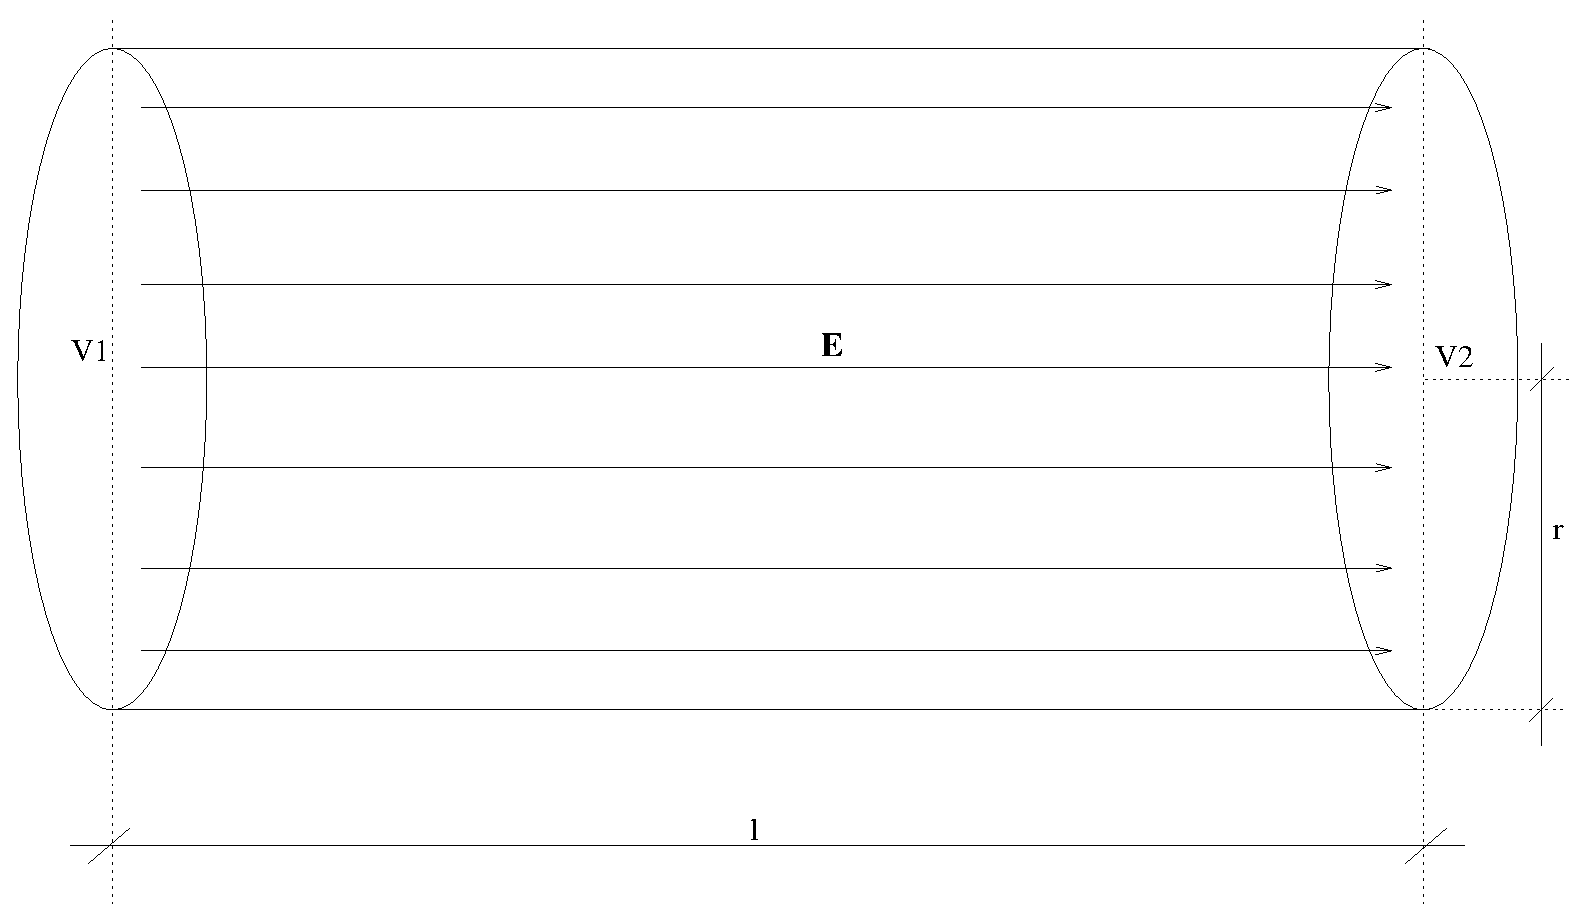
\includegraphics[scale=0.4]{immagini/fisica2/ohm1}
\end{figure}
Consideriamo un filo isotropo, omogeneo, di lunghezza $l$ e sezione $\Sigma$ variabile e con conduttività $\sigma$. Sia $\Delta V$ la differenza di potenziale mantenuta tra i due capi, con $V_1>V_2$. Consideriamo la differenza di potenziale tra due porzioni di superfici equipotenziali:
\begin{equation}
  \ud V = \ve E\cdot\ud \ve l = \frac{\ve J}{\sigma}\cdot\ud\ve l=\frac{\ve J}{\sigma}\cdot\ver n\,\ud l
\end{equation}
dove $\ver n$ è la normale alla superficie. Se integriamo sulla superficie:
\begin{equation}
  \int\ud V\,\ud\Sigma=\int\frac{\ve J}{\sigma}\cdot\ver n\,\ud l\,\ud\Sigma
\end{equation}
poiché la superficie su cui stiamo integrando è equipotenziale $\ud V$ è costante su tutta la superficie e può uscire dall'integrale:
\begin{equation}
  \ud V\int\ud\Sigma = \ud V\Sigma=\frac{\left[\int_\Sigma\ve J\cdot\ver n\, \ud \Sigma\right]\ud l}{\sigma} = \frac{I}{\sigma}\ud l
\end{equation}
e si è supposto che $\sigma$ sia anch'essa costante su tutta la superficie. Integrando su tutta la lunghezza del conduttore:
\begin{equation}
  \Delta V = \int\ud V=\int\frac{I}{\Sigma\sigma}\,\ud l
\end{equation}
Essendo gli elementini in serie la corrente è la stessa per tutti, mentre la sezione e la conducibilità potrebbero dipendere dalla posizione: $\sigma=\sigma(l)$, $\Sigma=\Sigma(l)$:
\begin{equation}
  \Delta V = I\int \frac{\ud l}{\Sigma\sigma}=IR
\end{equation}
\begin{Def}[resistenza elettrica\index{resistenza!elettrica}]
  \begin{equation}R=\int_A^B \frac{\rho}{\Sigma}\,\ud l\end{equation}
  dove l'integrale di cammino è fatto su un percoso normale alle superfici equipotenziali, ovvero parallelo al campo elettrico.
\end{Def}
\begin{legge}[Ohm]
  \begin{equation}
    \Delta V=IR
  \end{equation}
\end{legge}
che in realtà è stata introdotta come legge sperimentale. I materiali che rispettano questa legge sono detti ohmnici.\index{materiale ohmnico}
\begin{Es}[Filo]
  Un filo a sezione $S$, resistività $\rho$ entrambi costanti e lunghezza $L$, avrà resistenza:
  \begin{equation}
    R=\int_A^B \frac{\rho}{\Sigma}\ud l=\rho\frac{L}{S}
  \end{equation}
  \begin{figure}[htbp]
    \centering
    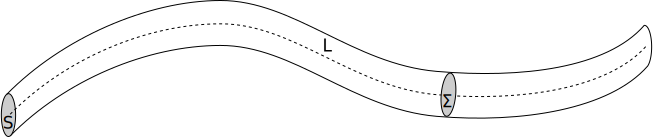
\includegraphics[scale=0.5]{immagini/fisica2/filo_serpente}
    % filo_serpente.pdf: 0x0 pixel, 0dpi, nanxnan cm, bb=
  \end{figure}
\end{Es}
\begin{Es}[Conduttori cilindrici]
  \begin{figure}[htbp]
    \centering
    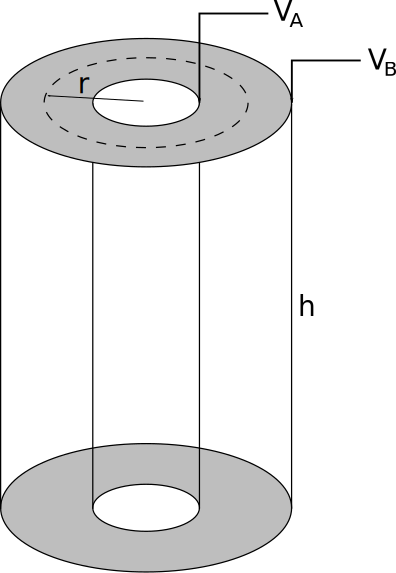
\includegraphics[scale=0.35]{immagini/fisica2/conduttore_cilindrico}
    % conduttore_cilindrico.pdf: 317x458 pixel, 72dpi, 11.18x16.16 cm, bb=0 0 317 458
  \end{figure}
  Consideriamo due superfici cilindriche concentriche, e tra queste inseriamo un materiale con resistività $\rho$ uniforme. Applichiamo una $\Delta V$ sulle due superfici, vogliamo sapere quanto è la corrente che scorre.
  \[
    R = \frac{\Delta V}{I} = \rho\int\frac{\ud l}{\Sigma(l)}
  \]
  dove $l$ è nella direzione radiale. Per la geometria dei conduttori
  \[
    \Sigma(r) = 2\pi rh
  \]
  \[
    R = \rho\int\frac{\ud r}{2\pi rh}=\frac{\rho}{2\pi h}\log\left(\frac{r_B}{r_A}\right)
  \]
  \[
    I = \frac{\Delta V}{R} = \Delta V \frac{2\pi h}{\rho\log\frac{r_B}{r_A}}
  \]
\end{Es}


\subsection{Temperatura}
La temperatura modifica $\rho$ in quanto al crescere della temperatura i nuclei degli elettroni si muovono più velocemente e gli urti con gli elettroni diventano più probabili. L'aumento di resistività del tipo:
\[\rho(T)=\rho_0\left[1+a\left(T-T_0\right)+b\left(T-T_0\right)^2+c\left(T-T_0\right)^3+\cdots\right]\]
di solito $a>b>c>\cdots$ e si considera solo il primo termine:
\[\rho(T)=\rho_0\left(1+\alpha\left(T-T_0\right)\right)\]
considerandolo come uno sviluppo di Taylor:
\[\alpha=\frac{1}{\rho_0}\left.\frac{\partial \rho}{\partial T}\right|_{T_0}\]
Per i semiconduttori \index{semiconduttori} $\alpha<0$. Ad una certa temperatura, detta temperatura critica\index{temperatura!critica}, la resistività crolla e si ha il fenomeno della superconduttività\index{superconduttività}\index{superconduttori}.

Il modello basato sul gas di elettroni non riesce a spiegare questo andamento, infatti:
\[v_T=\sqrt{3\frac{kT}{m_\mathrm{e}}}\]
cioè $\rho\propto v_T\propto\sqrt{T}$ invece che $\rho\propto T$. Inoltre non riesce a spiegare la diversità di $\rho$ tra i diversi materiali, sia conduttori che non, infatti
\[\rho=\frac{m_\mathrm{e}}{e^2N\tau}=\frac{m_\mathrm{e}}{eN}\frac{v_T}{l}\]
dice solo che la variazione tra i diversi materiali è data da $N$, che in realtà non varia di molto da conduttore a conduttore. Nella realtà $\rho$ è influenzato da numerosi fattori tra cui le impurezze cioè il disordine del reticolo.

\subsection{Resistori}
\begin{Def}[resistore\index{resistore}]
  Un resistore è un conduttore caratterizzato dal valore della resistenza\footnote{La resistenza è una grandezza, non è un conduttore}.
\end{Def}
\begin{Def}[rete resistiva\index{rete!resistiva}]
  Una rete resistiva è un insieme di resistori collegati insieme.
\end{Def}
\begin{Def}[circuito elettrico\index{circuito!elettrico}]
  Un circuito è una successione chiusa di resistori e generatori di forza elettromotrice, più eventuali altri elementi.
\end{Def}
\subsubsection{Resistori in serie e in parallelo}
\paragraph{Serie\index{resistori!in serie}}
I resistori si dicono collegati in serie quando sono attraversati tutti dalla stessa corrente. Applicando la legge di Ohm:
\[V_1-V_2=IR_1\qquad \cdots \qquad V_{n-1}-V_{n}=IR_n\]
Sommando tutte le espressioni si ottiene che la caduta di tensione ai capi della rete è
\[V_1-V_n=I\sum_{i=1}^N R_i\]
Quindi la resistenza equivalente, la resistenza di quel resistore che produce gli stessi effetti dei resistori in serie, è la somma delle resistenze.
\paragraph{Parallelo\index{resistori!in parallelo}}
I resistori si dicono collegai in parallelo quando ai capi di ogni resistore è applicata la stessa differenza di potenziale. Applicando ancora la legge di Ohm:
\[\frac{V_1-V_2}{R_1}=I_1\qquad\cdots\qquad\frac{V_1-V_2}{R_n}=I_n\]
Sommando si ottiene che il reciproco del resistore equivalente è la somma dei reciproci dei resistori in parallelo.
\[
  V_1(1/R_1+1/R_2+\cdots)-V_2(1/R_1+1/R_2+\cdots) = (V_1 - V_2) \sum 1/R_i  = I
\]
\[
  V_1 - V_2 = I \left( \sum 1/R_i \right)^{-1}
\]
\begin{Es}[resistenza corpo esteso]
  \begin{figure}[htbp]
    \centering
    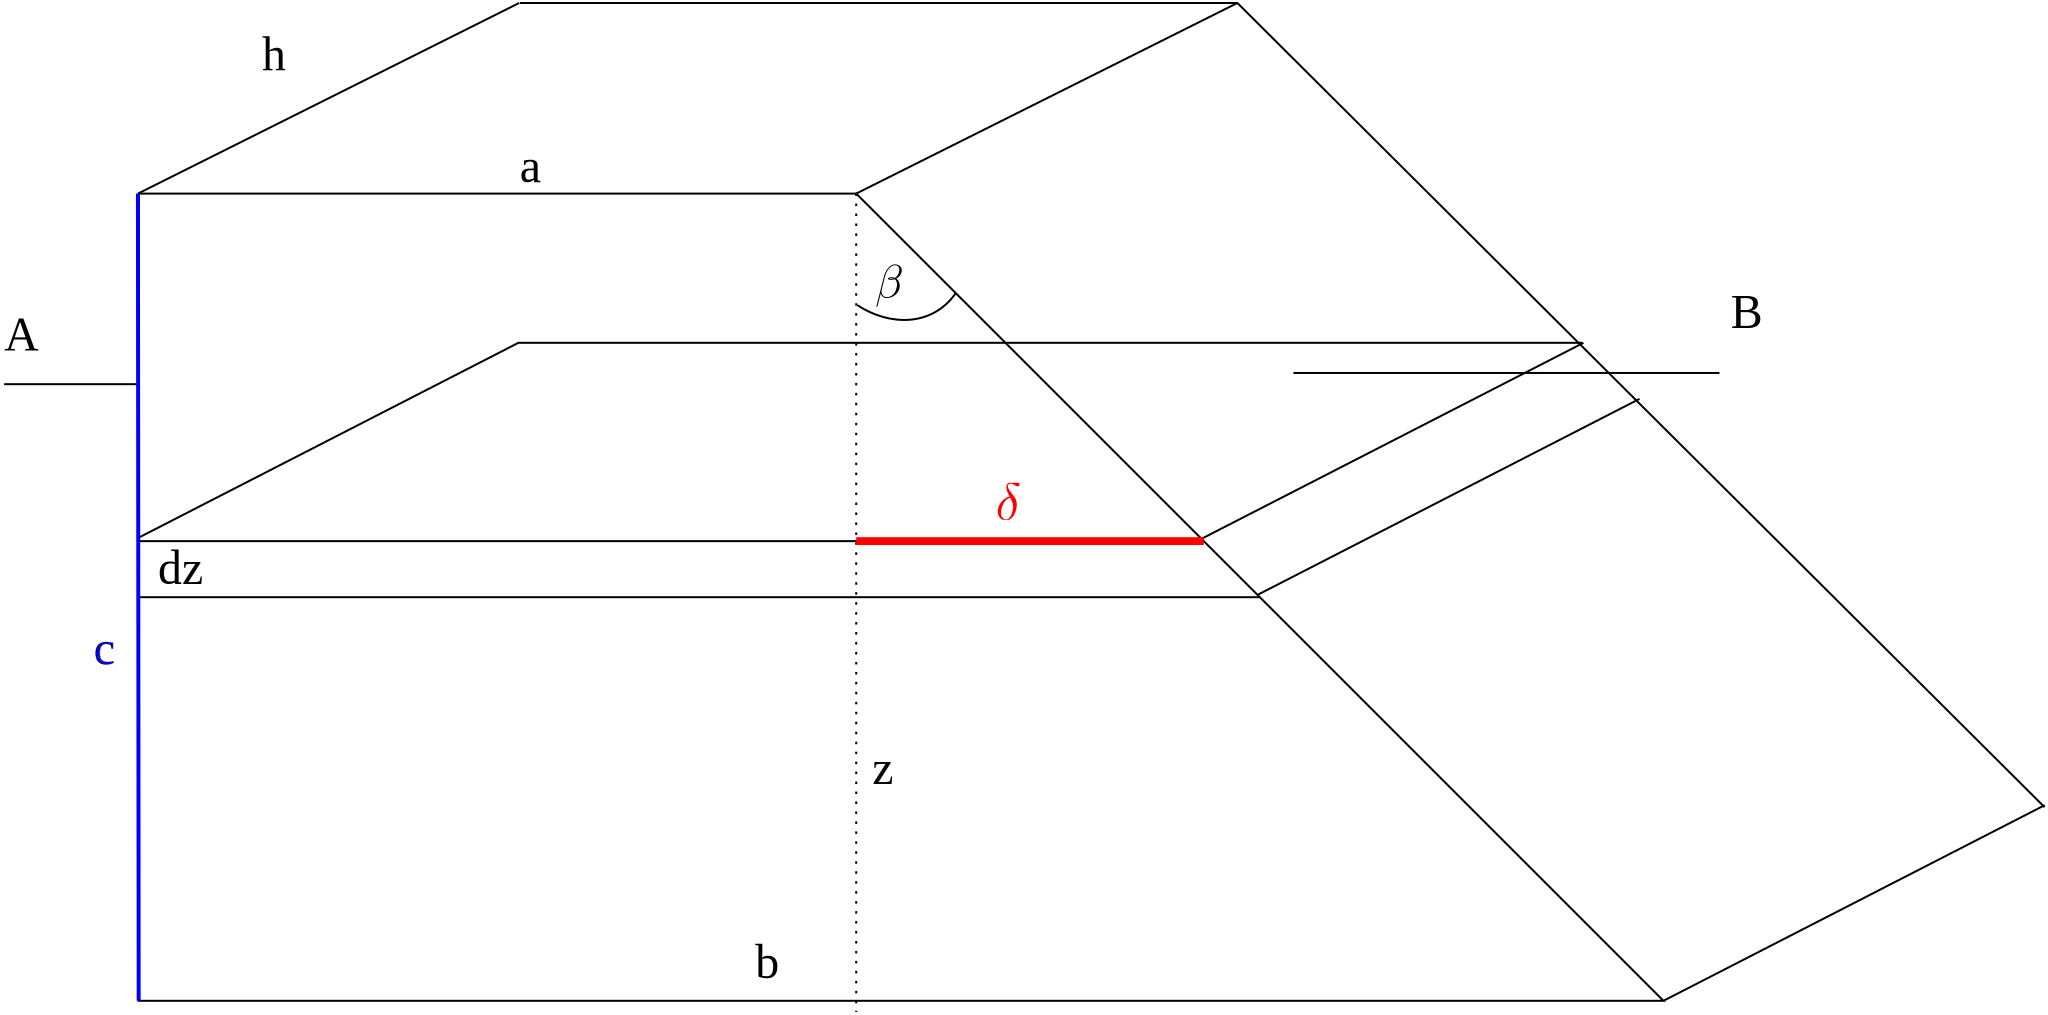
\includegraphics[scale=0.5]{immagini/fisica2/res_trapezio}
    \caption{resistenza di un corpo esteso.}
    \label{res_trapezio}
  \end{figure}
  Consideriamo il corpo in figura \eqref{res_trapezio}. Vogliamo calcolare la resistenza tra i capi $A$ e $B$. Scomponiamo la geometria in tanti elementini di altezza $\ud z$, essi risultano in parallelo. La loro resistenza:
  \[\ud R=\rho\frac{l}{A}=\rho\frac{y}{h\ud z}\]
  con $y=a+\delta$ che varia tra $a$ e $b$. Troviamo $\delta$:
  \[
    (c-z)\tan\beta=\delta\qquad c\tan\beta=b-a\qquad \delta=(c-z)\frac{b-a}{c}
  \]
  Allora $y$:
  \[y=a+\delta=a+\frac{(c-z)(b-a)}{c}=b+\frac{z}{c}(a-b)\qquad\ud y=\frac{a-b}{c}\ud z\]
  \[\frac{1}{R}=\int_0^c\frac{1}{\ud R}=\int_0^c\frac{h\ud z}{\rho y}=\frac{hc}{\rho(a-b)}\int_b^a\frac{\ud y}{y}=\frac{hc}{\rho(a-b)}\log\frac{a}{b}\]
  \[R=\frac{\rho(a-b)}{hc\log\frac{a}{b}}\]


\end{Es}


\section{Tempo di rilassamento\index{tempo!di rilassamento!di un conduttore}}
Vogliamo sapere quanto è il tempo necessario per un conduttore per eliminare un eccesso di carica. Consideriamo un conduttore isotropo, omogeneo, lineare, con conducibilità $\sigma$, con un eccesso di carica al tempo zero $\rho_0(\ve r)$ in una regione limitata di spazio. Si creerà un campo elettrico e quindi una densità di corrente $\ve J=\sigma\ve E$. Vogliamo studiare l'evolversi di $\rho(\ve r,t)$. Sappiamo:
\[\diver\ve E=\frac{\rho(\ve r,t)}{\varepsilon_0}\qquad\diver\ve J=-\frac{\partial\rho(\ve r,t)}{\partial t}\]
Essendo $\ve J=\sigma\ve E$:
\[\sigma\diver\ve E=-\frac{\partial\rho}{\partial t}\]
Sostituendo:
\[\frac{\sigma}{\varepsilon_0}\rho=-\frac{\partial\rho}{\partial t}\]
Risolvendo:
\[\frac{\ud\rho}{\rho}=-\frac{\sigma}{\varepsilon_0}\ud t\qquad \log\rho=-\frac{\sigma}{\varepsilon_0}t+c\qquad \rho=Ae^{-\frac{\sigma}{\varepsilon_0}t}=\rho_0 e^{-\frac{\sigma}{\varepsilon_0}t}\]
Chiamando $\tau=\frac{\sigma}{\varepsilon_0}$ tempo caratteristico, o tempo di rilassamento:
\[\rho=\rho_0e^{-\tau t}\]
Il tempo caratteristico \index{tempo!caratteristico} è quel tempo dopo il quale la densità di carica si è ridotta di $\frac{1}{e}$. Dopo qualche $\tau$ possiamo considerare tutto l'eccesso di carica eliminato.

\section{Generatori\index{generatori}}
Con un campo elettrostatico si possono creare correnti, come visto nel paragrafo precedente, ma non mantenerle in quanto il fenomeno si esaurisce in pochissimo tempo. I generatori possono mantenere una differenza di potenziale costate tra i poli o morsetti o variarla secondo una funzione, tipicamente sinusoidale. Nel primo caso si parla di pile\index{pila} o batterie\index{batteria}. In un circuito chiuso:
\[\oint_C\ve E\cdot\ud\ve l=0\]
Essendo $\ve J=\sigma \ve E$:
\[\oint_C\ve J\cdot\ud\ve l=\sigma\oint_C\ve E\cdot\ud\ve l=0\]
\`E assurdo perché non ci sarebbe corrente. Dobbiamo supporre ci siano alte forze, non conservative, che non sono svolte dal campo elettrostatico, essendo il suo lavoro nullo. Tali forze sono localizzate nel generatore. Consideriamo allora un a altro campo $E_i$, il campo elettrico impresso \index{campo!elettrico!impresso}o elettromotore \index{campo!elettromotore}che si somma al campo elettrostatico:
\[\ve E_T=\ve E+\ve E_i\qquad \ve J=\sigma(\ve E+\ve E_i)\]
Il campo impresso nasce quando si è in presenza di una disomogeneità  come ad esempio all'interno della pila.
\begin{figure}[htbp]
  \centering
  \includegraphics[scale=2]{immagini/fisica2/generatore}
  \caption{simbolo della pila.}
\end{figure}

Calcoliamo il lavoro fatto dai due campi su una carica unitaria all'interno di un circuito chiuso:
\begin{equation}
  L = \oint (\ve E+\ve E_i)\cdot\ud\ve l = \oint \ve E_i\cdot\ud\ve l = \int_{\text{pila}}\!\!\!\! \ve E_i\cdot\ud\ve l + \int_{\text{circuito}} \underbrace{\ve E_i}_{=0}\cdot\ud\ve l = \int_{\text{pila}}\!\!\!\!\ve E_i\cdot\ud\ve l
\end{equation}
avendo notato che la circuitazione del campo elettrostatico è nulla, mentre il campo impresso è nullo all'esterno della pila.
\begin{Def}[fem]
  La forza elettromotrice\index{forza!elettromotrice} è il lavoro fatto dal campo totale $\ve E+\ve E_i$ su una carica positiva unitaria che percorra una linea chiusa che passi per gli elettrodi della pila:
  \begin{equation}
    \text{fem} = \int_{\text{pila}} \ve E_i\cdot\ud\ve l
  \end{equation}

\end{Def}

\subsection{Resistenza interna}
Ogni generatore reale è caratterizzato da una resistenza interna $r$ e da una forza elettromotrice $\varepsilon$. Se gli colleghiamo un resistore con resistenza $R$ la circuitazione del campo elettrostatico deve essere nulla e quindi anche la variazione di potenziale. Allora se ai capi del generatore ideale c'è una differenza di potenziale $\varepsilon$ la caduta di tensione attraverso $R$ e $r$ deve essere uguale e contraria a $\varepsilon$. La differenza di tensione del generatore reale è minore di quella del generatore ideale e in particolare:
\[V_2-V_1=\varepsilon-Ir\]

Se in un ramo di circuito con estremi $A$ e $B$ ci sono dei resistori in serie e un generatore vale:
\begin{legge}[Ohm generalizzata\index{legge!di Ohm!generalizzata}]
  \begin{equation}
    V_A-V_B+\varepsilon=IR
    \label{Ohm_gen}
  \end{equation}
  con $R=\sum R_i+r$.
\end{legge}
\subsubsection{Potenza massima}
Vogliamo sapere quando un circuito assorbe la potenza massima. Riassumiamo tutto il circuito con un resistore con resistenza $R$, che rappresenta il carico cioè tutte le resistenze collegate al generatore reale, un generatore ideale e una resistenza interna $r$. Sappiamo che la potenza è
\[P=RI^2=R\left(\frac{\varepsilon}{R+r}\right)^2\]
Vogliamo sapere qual è l'$R$ ottimale per cui viene dissipata la potenza maggiore su $R$. Deriviamo in $R$:
\[\frac{\ud P}{\ud R}=\varepsilon^2\left[\frac{1}{(R+r)^2}-\frac{2R}{(r+R)^3}\right]\]
che ha uno zero per $r=R$.

Se $r$ è molto diverso da $R$ gran parte dell'energia viene dispersa su $r$, cioè all'interno del generatore.

\section{Effetto Joule\index{effetto!Joule}\index{Joule}}
L'effetto Joule può essere spiegato sia da un punto di vista macroscopico che microscopico utilizzando il modello del gas di elettroni liberi. L'effetto Joule avviene ogni qualvolta la corrente passa attraverso un resistore.
\subsection{Macroscopico}
Quando una carica $\ud q$ passa da un potenziale $V_B$ a un potenziale $V_A$ ci sarà una variazione di energia potenziale; per definizione:
\[\ud W=\ud q(V_B-V_A)\]
ma $\ud q=I(t)\ud t$, sostituendo:
\begin{legge}[Joule\index{legge!di Joule}]
  \begin{equation}
    \ud W=I(t)(V_B-V_A)\ud t
  \end{equation}
\end{legge}
\subsubsection{corrente stazionaria}
Nel caso stazionario $I(t)=I$:
\[W=\int_0^t I(V_B-V_A)\ud t=I(V_B-V_A)t\]
se il conduttore è ohmnico $I=\frac{\Delta V}{R}$:
\[W=RI^2t\]
e la potenza:
\[P=\frac{\ud W}{\ud t}=I\Delta V=RI^2=\frac{\Delta V^2}{R}\]

\subsection{Microscopico}
Consideriamo un conduttore con $N$ portatori di carica nell'unità di volume.
\[
  L_e=\ve F\cdot\ve s
\]
la potenza:
\[
  P_e =\ve F\cdot\ve v
\]
considerando tutti gli elettroni nel volume $\ud v$, la potenza:
\[
  \ud P=\ve F\cdot\ve v=-eN\ud v\ve E\cdot \ve v = \ve E\cdot\ve J\ud v =\sigma E^2\ud v
\]
Si puo anche ragiornare come segue.  Il singolo elettrone ha in media $\tau^{-1}$ collisioni nell'unità di tempo. Quindi nell'elementino di volume $\ud v$ nel tempo $\ud t$ avvengono $N\frac{\ud v}{\tau}\ud t$ collisioni. Tra un urto e un altro un elettrone viene accelerato con una forza $-eE$ parallela al campo elettrico costante. Lo spostamento sarà $v_D\tau$ parallelo al campo elettrico. Allora il lavoro su un elettrone sarà
\[
  \ud L_e =\ve F\cdot\ve s=-e Ev_D\ud t
\]
e su tutti gli elettroni nel volume $\ud v$:
\[
  \ud L = -e Ev_D\ud t N\ud v
\]
Considerando tutti gli elettroni del volume $\ud v$ la potenza:
\[
  \ud P=-\frac{N\ud v}{\tau}eEv_d\tau
\]
Ricordando che:
\[v_D=-\frac{eE}{m\tau}\qquad\sigma=\frac{e^2N}{m}\tau\]
\[\ud P=\frac{e^2NE^2}{m}\tau\ud v=\sigma E^2\ud v\]
Se consideriamo un filo conduttore di lunghezza $l$ e sezione $S$ con una differenza di potenziale $V_A-V_B=El$.
\[P=\int_V\ud P=\sigma E^2\int_V\ud v=\sigma E^2(Sl)=\sigma\frac{\Delta V^2}{l^2}Sl=\sigma\frac{S}{l}\Delta V^2=\frac{\Delta V^2}{R}\]

